\documentclass[12pt]{article}
\usepackage[a4paper,margin=1in,footskip=0.25in]{geometry} % set margins
\usepackage[portuguese]{babel}
\usepackage[utf8]{inputenc}
\usepackage[hidelinks]{hyperref} 
\usepackage{amsmath}
\usepackage{amssymb}
\usepackage{amsthm}
\usepackage{graphicx}    % needed for include graphics
\usepackage{subfigure}   % add subfigures
\usepackage{indentfirst}
\usepackage{float}       % needed for [H] figure placement option
\usepackage{setspace}    % needed for doublespacing
\usepackage{tikz}
\usepackage{algpseudocode}
\usepackage{listings}
\usepackage{xcolor}

\definecolor{mGreen}{rgb}{0,0.6,0}
\definecolor{mGray}{rgb}{0.5,0.5,0.5}
\definecolor{mPurple}{rgb}{0.58,0,0.82}
\definecolor{backgroundColour}{rgb}{0.95,0.95,0.92}

\lstdefinestyle{CStyle}{
    backgroundcolor=\color{backgroundColour},   
    commentstyle=\color{mGreen},
    keywordstyle=\color{magenta},
    numberstyle=\tiny\color{mGray},
    stringstyle=\color{mPurple},
    basicstyle=\footnotesize,
    breakatwhitespace=false,         
    breaklines=true,                 
    captionpos=b,                    
    keepspaces=true,                 
    numbers=left,                    
    numbersep=5pt,                  
    showspaces=false,                
    showstringspaces=false,
    showtabs=false,                  
    tabsize=2,
    language=C
}

% Macros
\renewcommand{\familydefault}{\sfdefault} % sans-serif
\newcommand{\lowtext}[1]{$_{\text{#1}}$}
\newcommand{\code}[1]{\texttt{#1}}

% Adds ./img/ to the path of figures
\graphicspath{{./img/}}

\title{Relatório EP1 - MAC0219}
\author{Bruno Sesso, Gustavo Estrela de Matos, Lucas Sung Jun Hong}

\begin{document}
% Espaçamento duplo 
\doublespacing
\begin{titlepage}
    \vfill
    \begin{center}
        \vspace{0.5\textheight}
        \noindent
        Instituto de Matemática e Estatística \\
        EP1 - MAC0219 \\
        \vfill
        \noindent
        {\Large Cálculo do Conjunto de Mandelbrot
        em Paralelo com Pthreads e OpenMP} \\
        \bigskip
        \bigskip
        \begin{tabular}{ll}
            {\bf Professor:} & {Alfredo Goldman} \\
            {\bf Alunos:}    & {Bruno Sesso} \\
                             & {Gustavo Estrela de Matos} \\
                             & {Lucas Sung Jun Hong} \\
        \end{tabular} \\
        \vspace{\fill}
       \bigskip
        São Paulo, \today \\
       \bigskip
    \end{center}
\end{titlepage}

\pagebreak
\tableofcontents
\pagebreak

\section{Introdução}
Esse trabalho tem como objetivo implementar e analisar duas versões
paralelas de um código sequencial que é capaz de calcular o conjunto de
maldelbrot para diversas regiões do plano complexo. As duas versões do
código foram implementadas utilizando as bibliotecas OpenMP e PThreads.

Ao longo desse trabalho, iremos apresentar resultados de tempo de 
execução das diferentes implementações e suas respectivas variações.
Para isso, utilizamos a ferramenta {\em perf}, capaz de realizar 
repetições de experimentos, apresentando resultados médios e com desvio
padrão. Todos os resultados apresentados aqui foram feitos a partir de
no mínimo 10 execuções do mesmo comando.


    {\bf Por que é recomendado realizar mais de uma medição?} 
        Porque os resultados observados dependem do estado da máquina
        durante a execução do programa. Como testamos nossos programas
        em máquinas com um sistema operacional, rodando diversos outros
        programas ao mesmo tempo, é esperado que fatores como fila de
        processos, paginação de memória, etc, interfira no tempo de 
        execução do nosso programa. Portanto, se tiramos uma média
        de várias execuções, somos capazes de dizer aproximadamente
        o comportamento médio do programa.
        

%%%%%%%%%%%%%%%%%%%%% SEQUENCIAL %%%%%%%%%%%%%%%%%%%%%%%%%%%%%%
\newpage
\section{Código Sequencial}
Para implementar a versão sequencial do programa do cálculo do conjunto de Mandelbrot temos uma versão com alocação de memória e com comandos de leitura e escrita e uma versão sem ambos. No caso sem ambos, como não há comandos de leitura, os comandos de leitura e escrita são retirados, removendo-se a função \code{write\_to\_file()}. Para a remoção de alocação de memória pode ser que o tempo de acesso a um vetor possa ser relevante, portanto não simplesmente removemos a função de alocação de memória. Para retirar as alocações, supomos que o tamanho máximo de uma imagem será de 11500px x 11500px e assim substituimos a alocação dinâmica do \code{image\_buffer} por uma alocação estática: \code{char image\_buffer[11500*11500][3]}.

Comparemos os resultados obtidos nos testes com e sem alocação de memória e comandos de leitura e escrita:

\begin{figure}[H]
    \makebox[\textwidth][c]{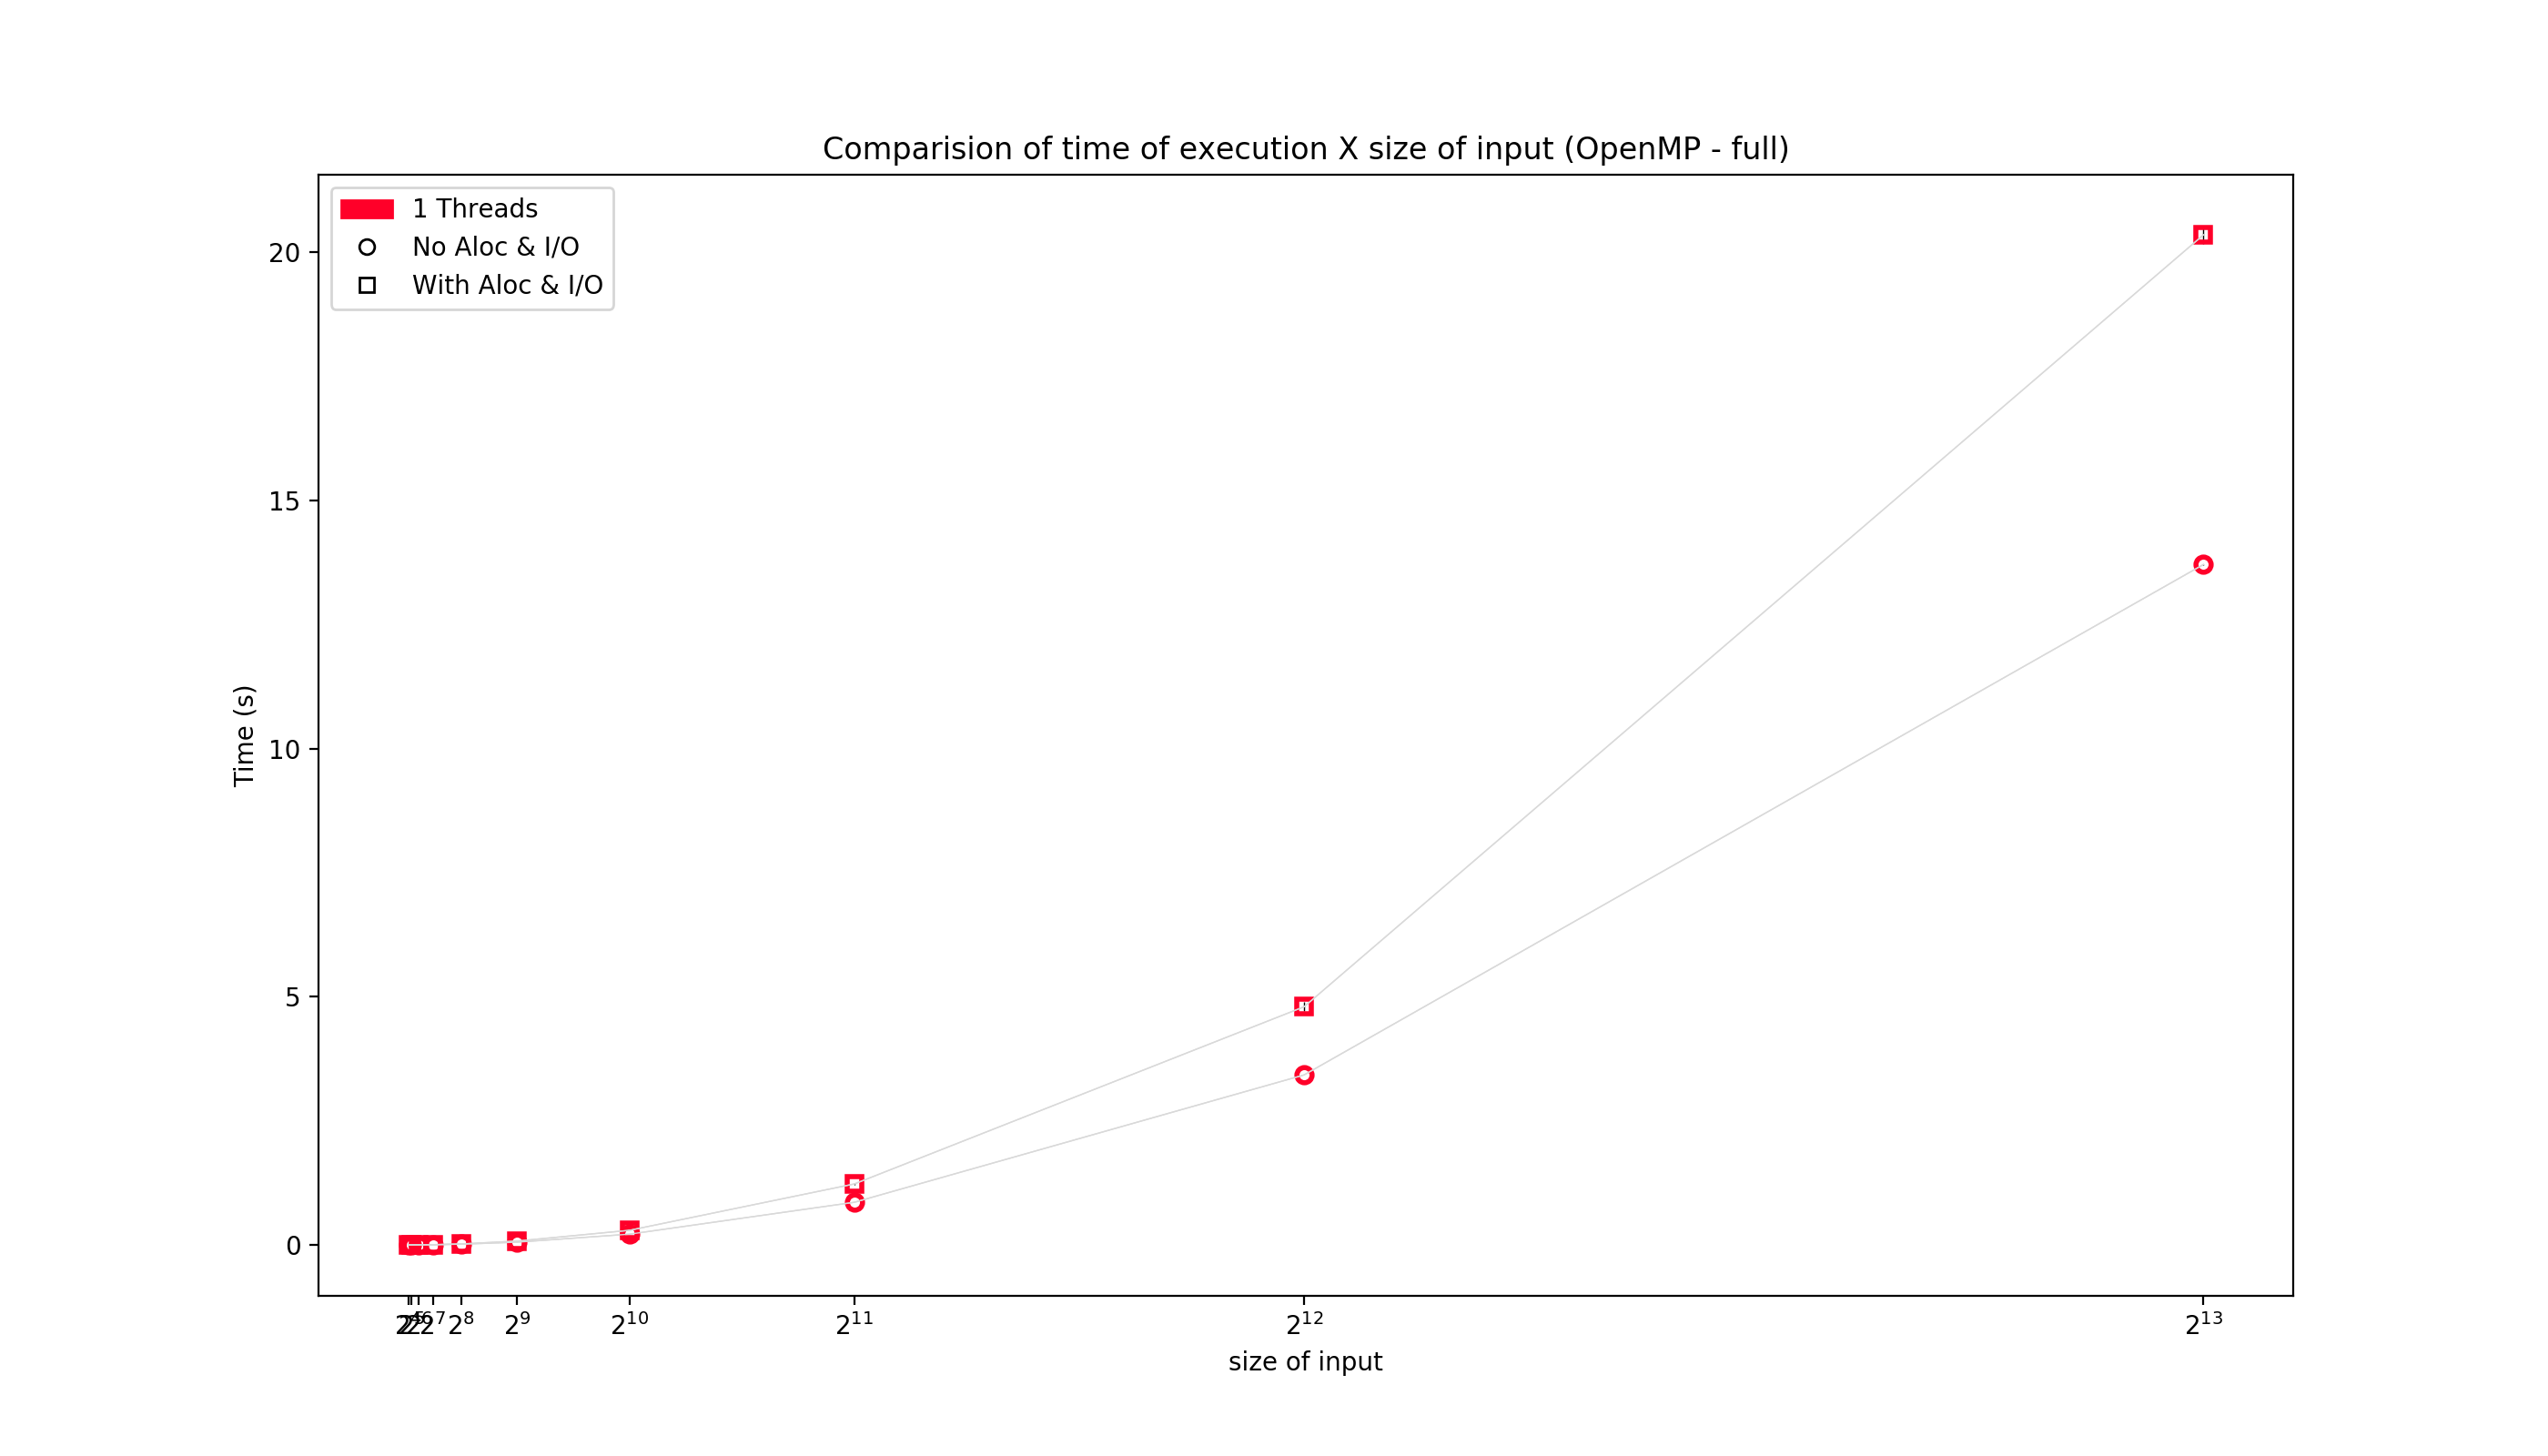
\includegraphics[scale=.60]{seq_comp/compare_timeXsize_full_OpenMPpng.png}}
\end{figure}

Como esperado o tempo do programa sem alocação e sem comandos de leitura e escrita é consideravelmente menor que a versão com. Nas demais regiões o comportamento se repete:

\begin{figure}[H]
    \makebox[\textwidth][c]{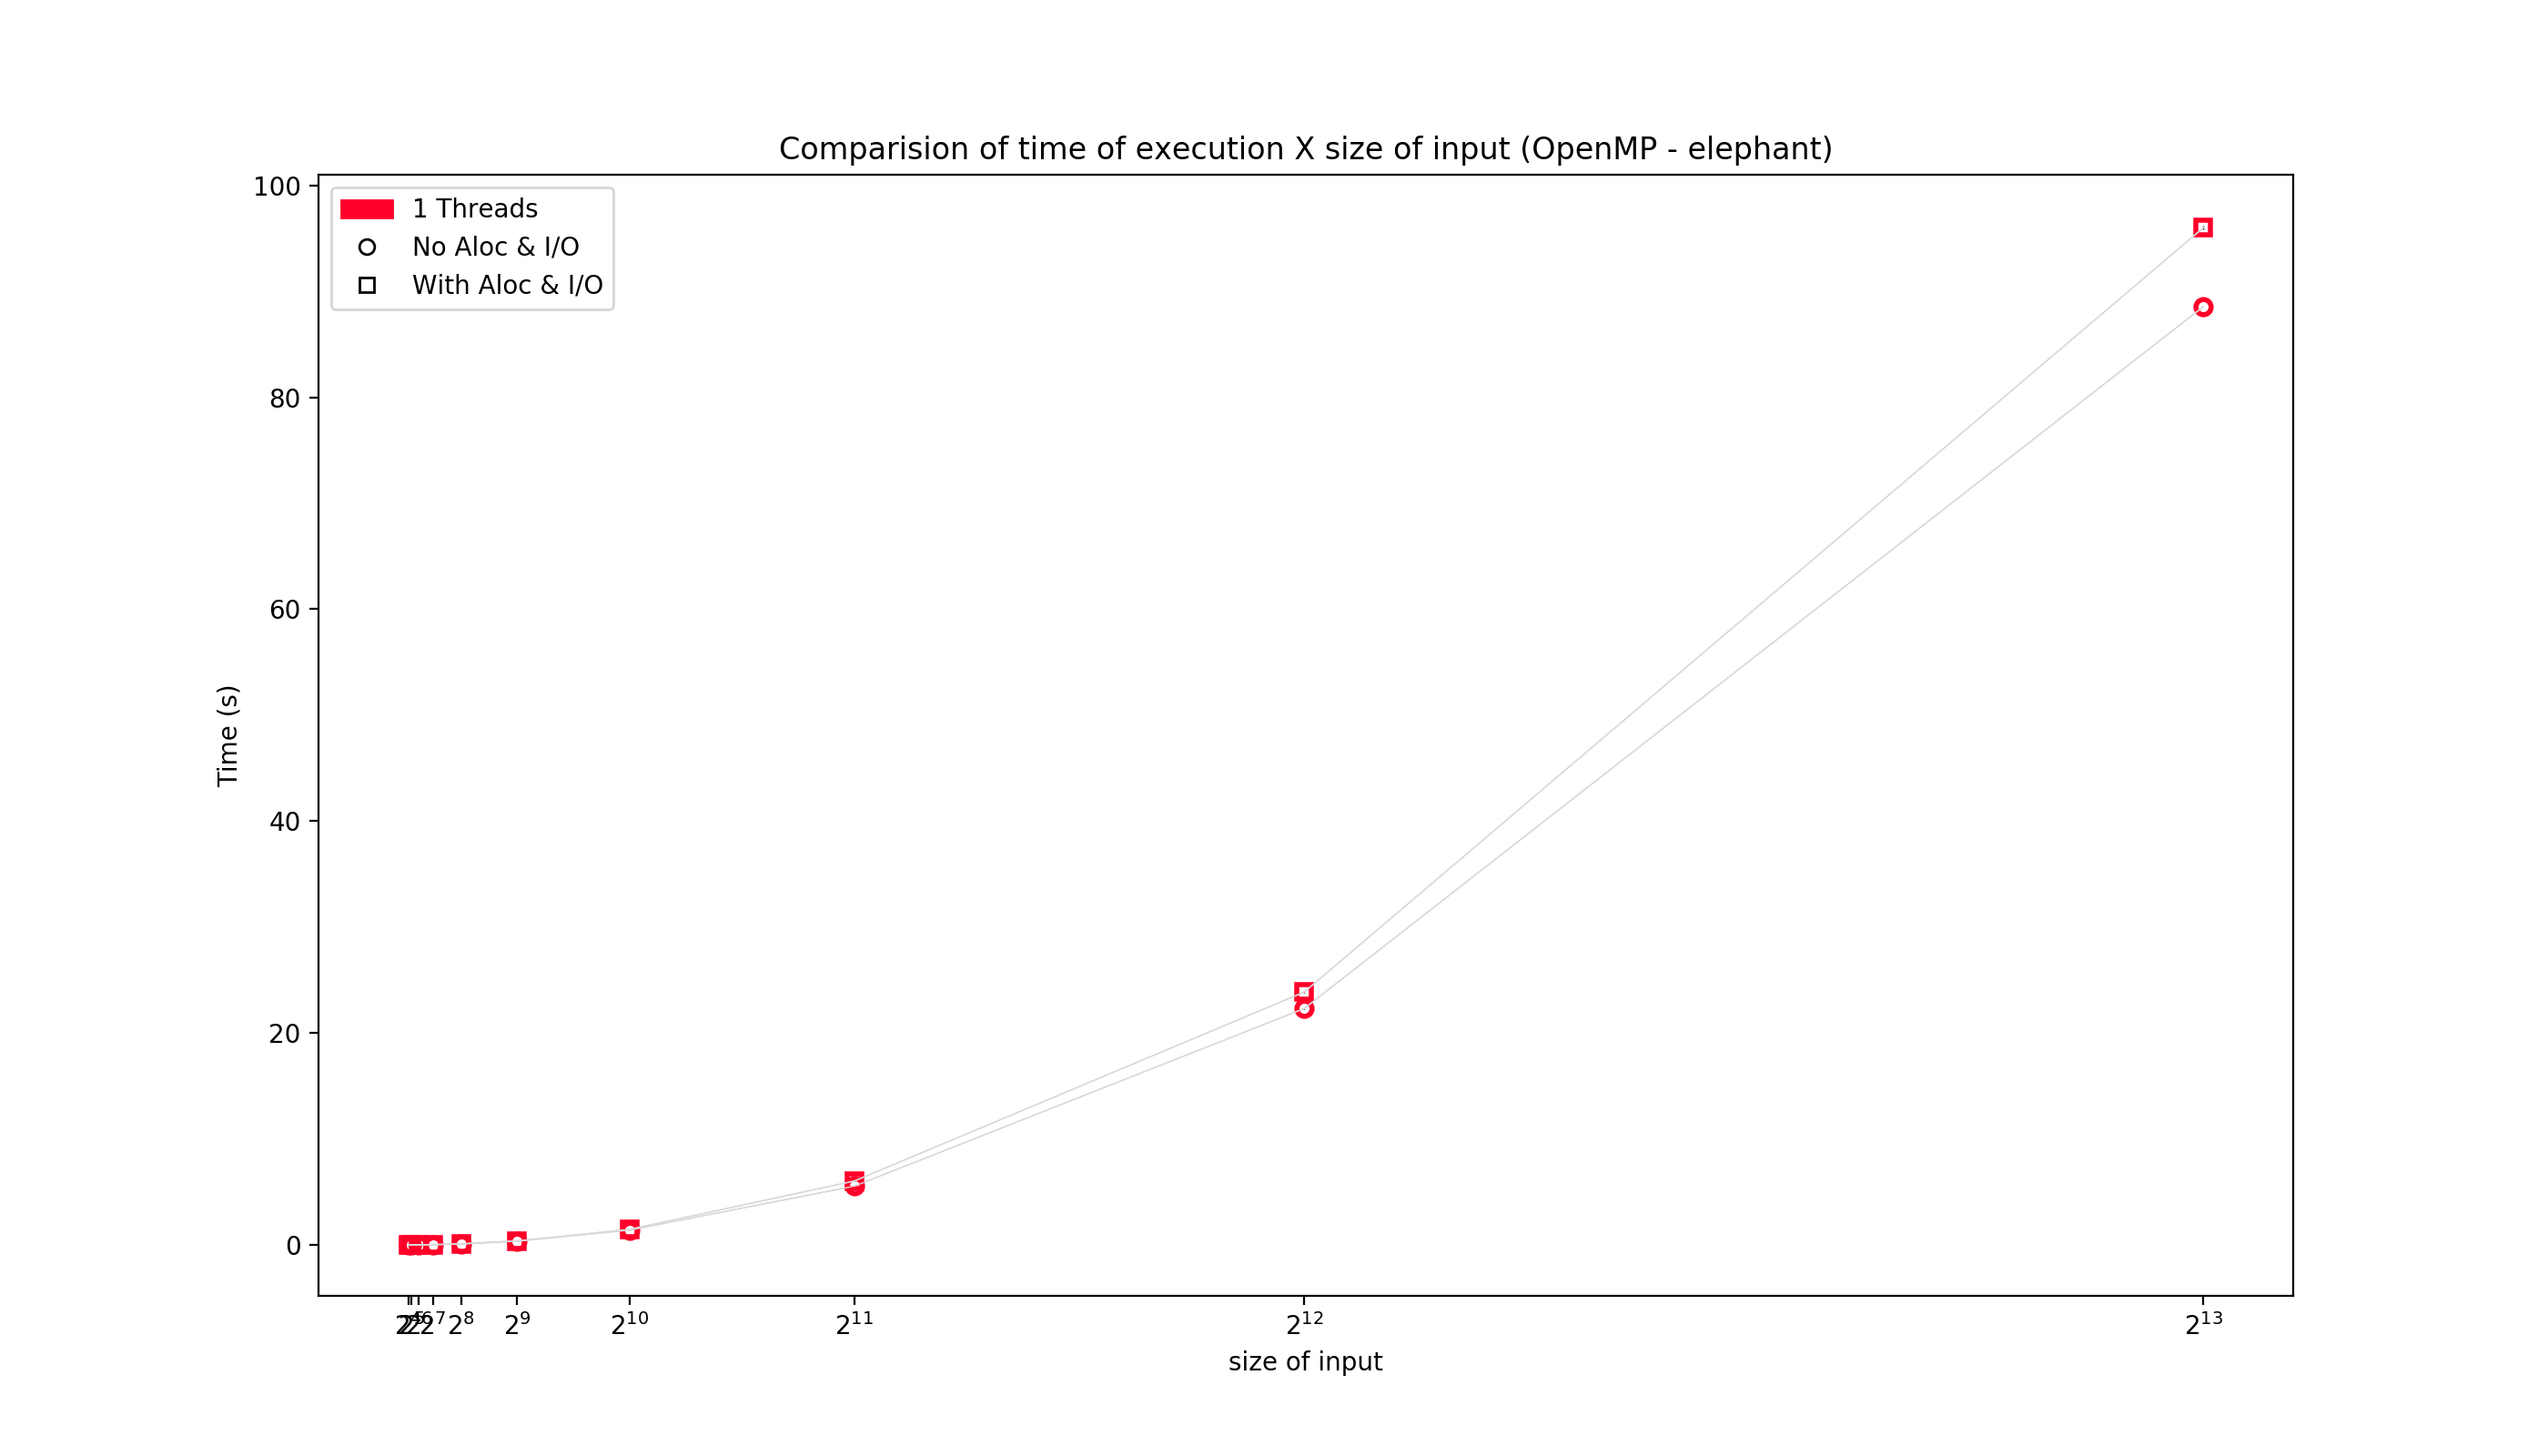
\includegraphics[scale=.50]{seq_comp/compare_timeXsize_elephant_OpenMPpng.png}}
\end{figure}
\begin{figure}[H]
    \makebox[\textwidth][c]{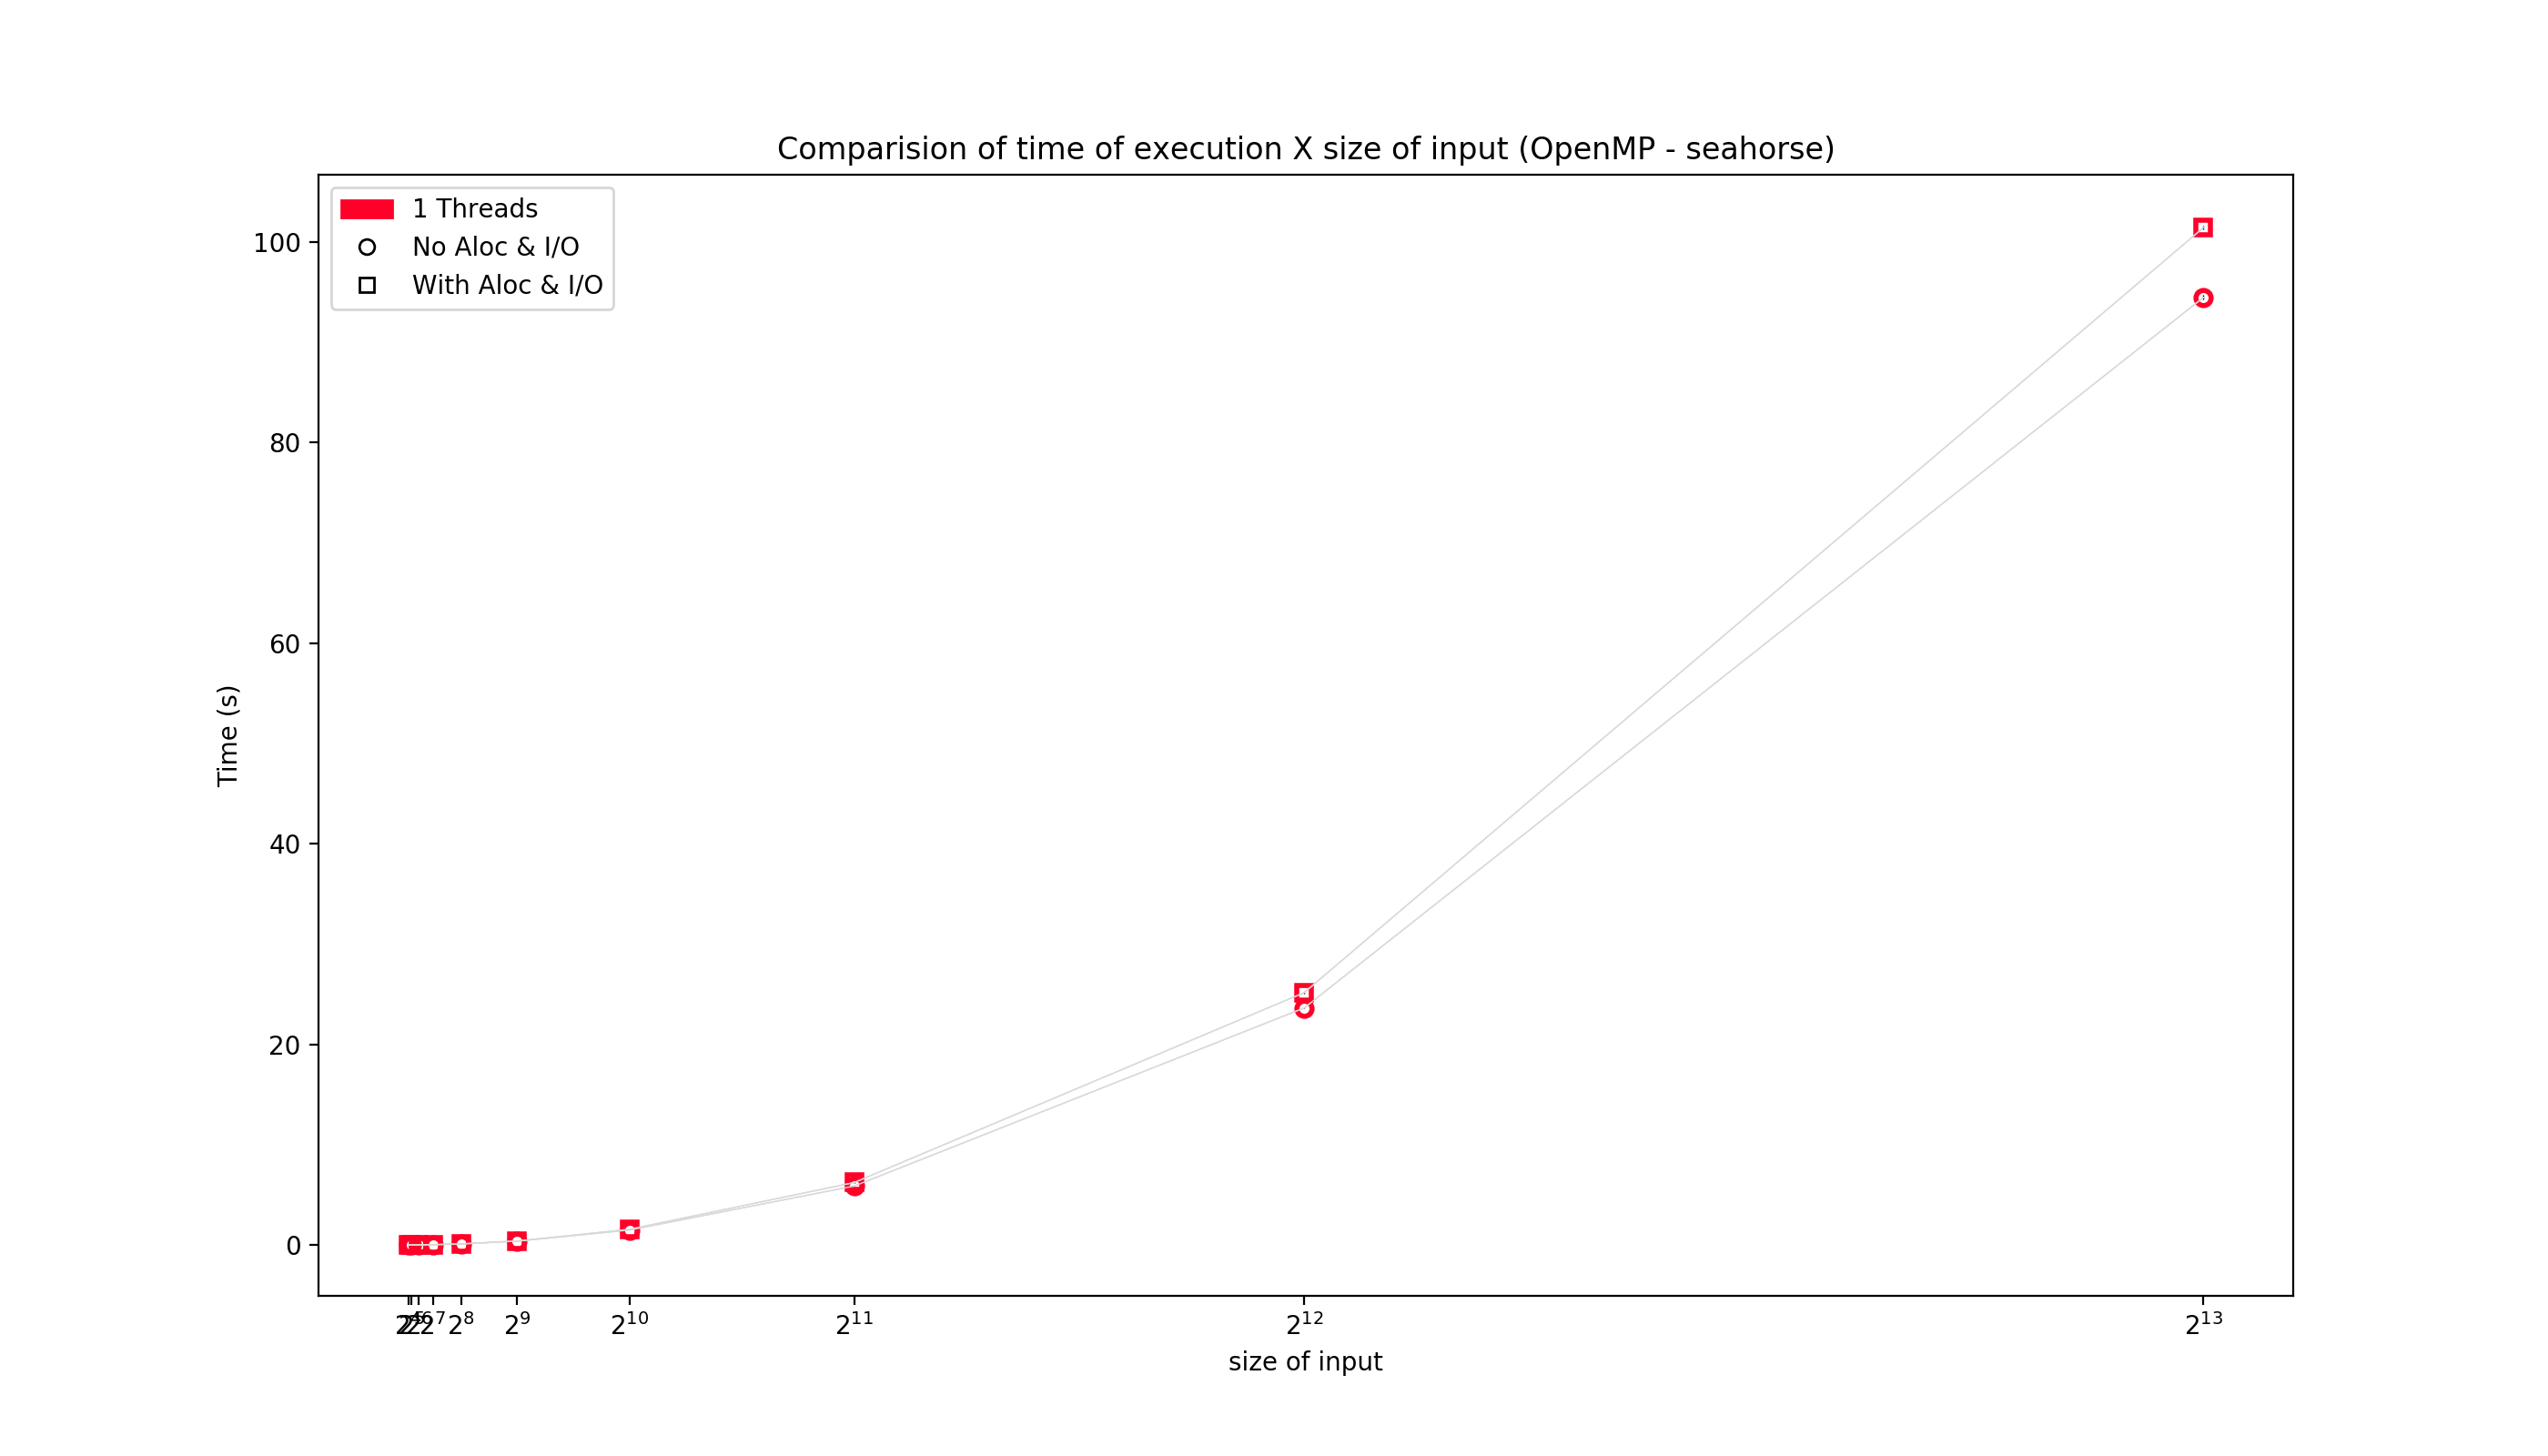
\includegraphics[scale=.50]{seq_comp/compare_timeXsize_seahorse_OpenMPpng.png}}
\end{figure}
\begin{figure}[H]
    \makebox[\textwidth][c]{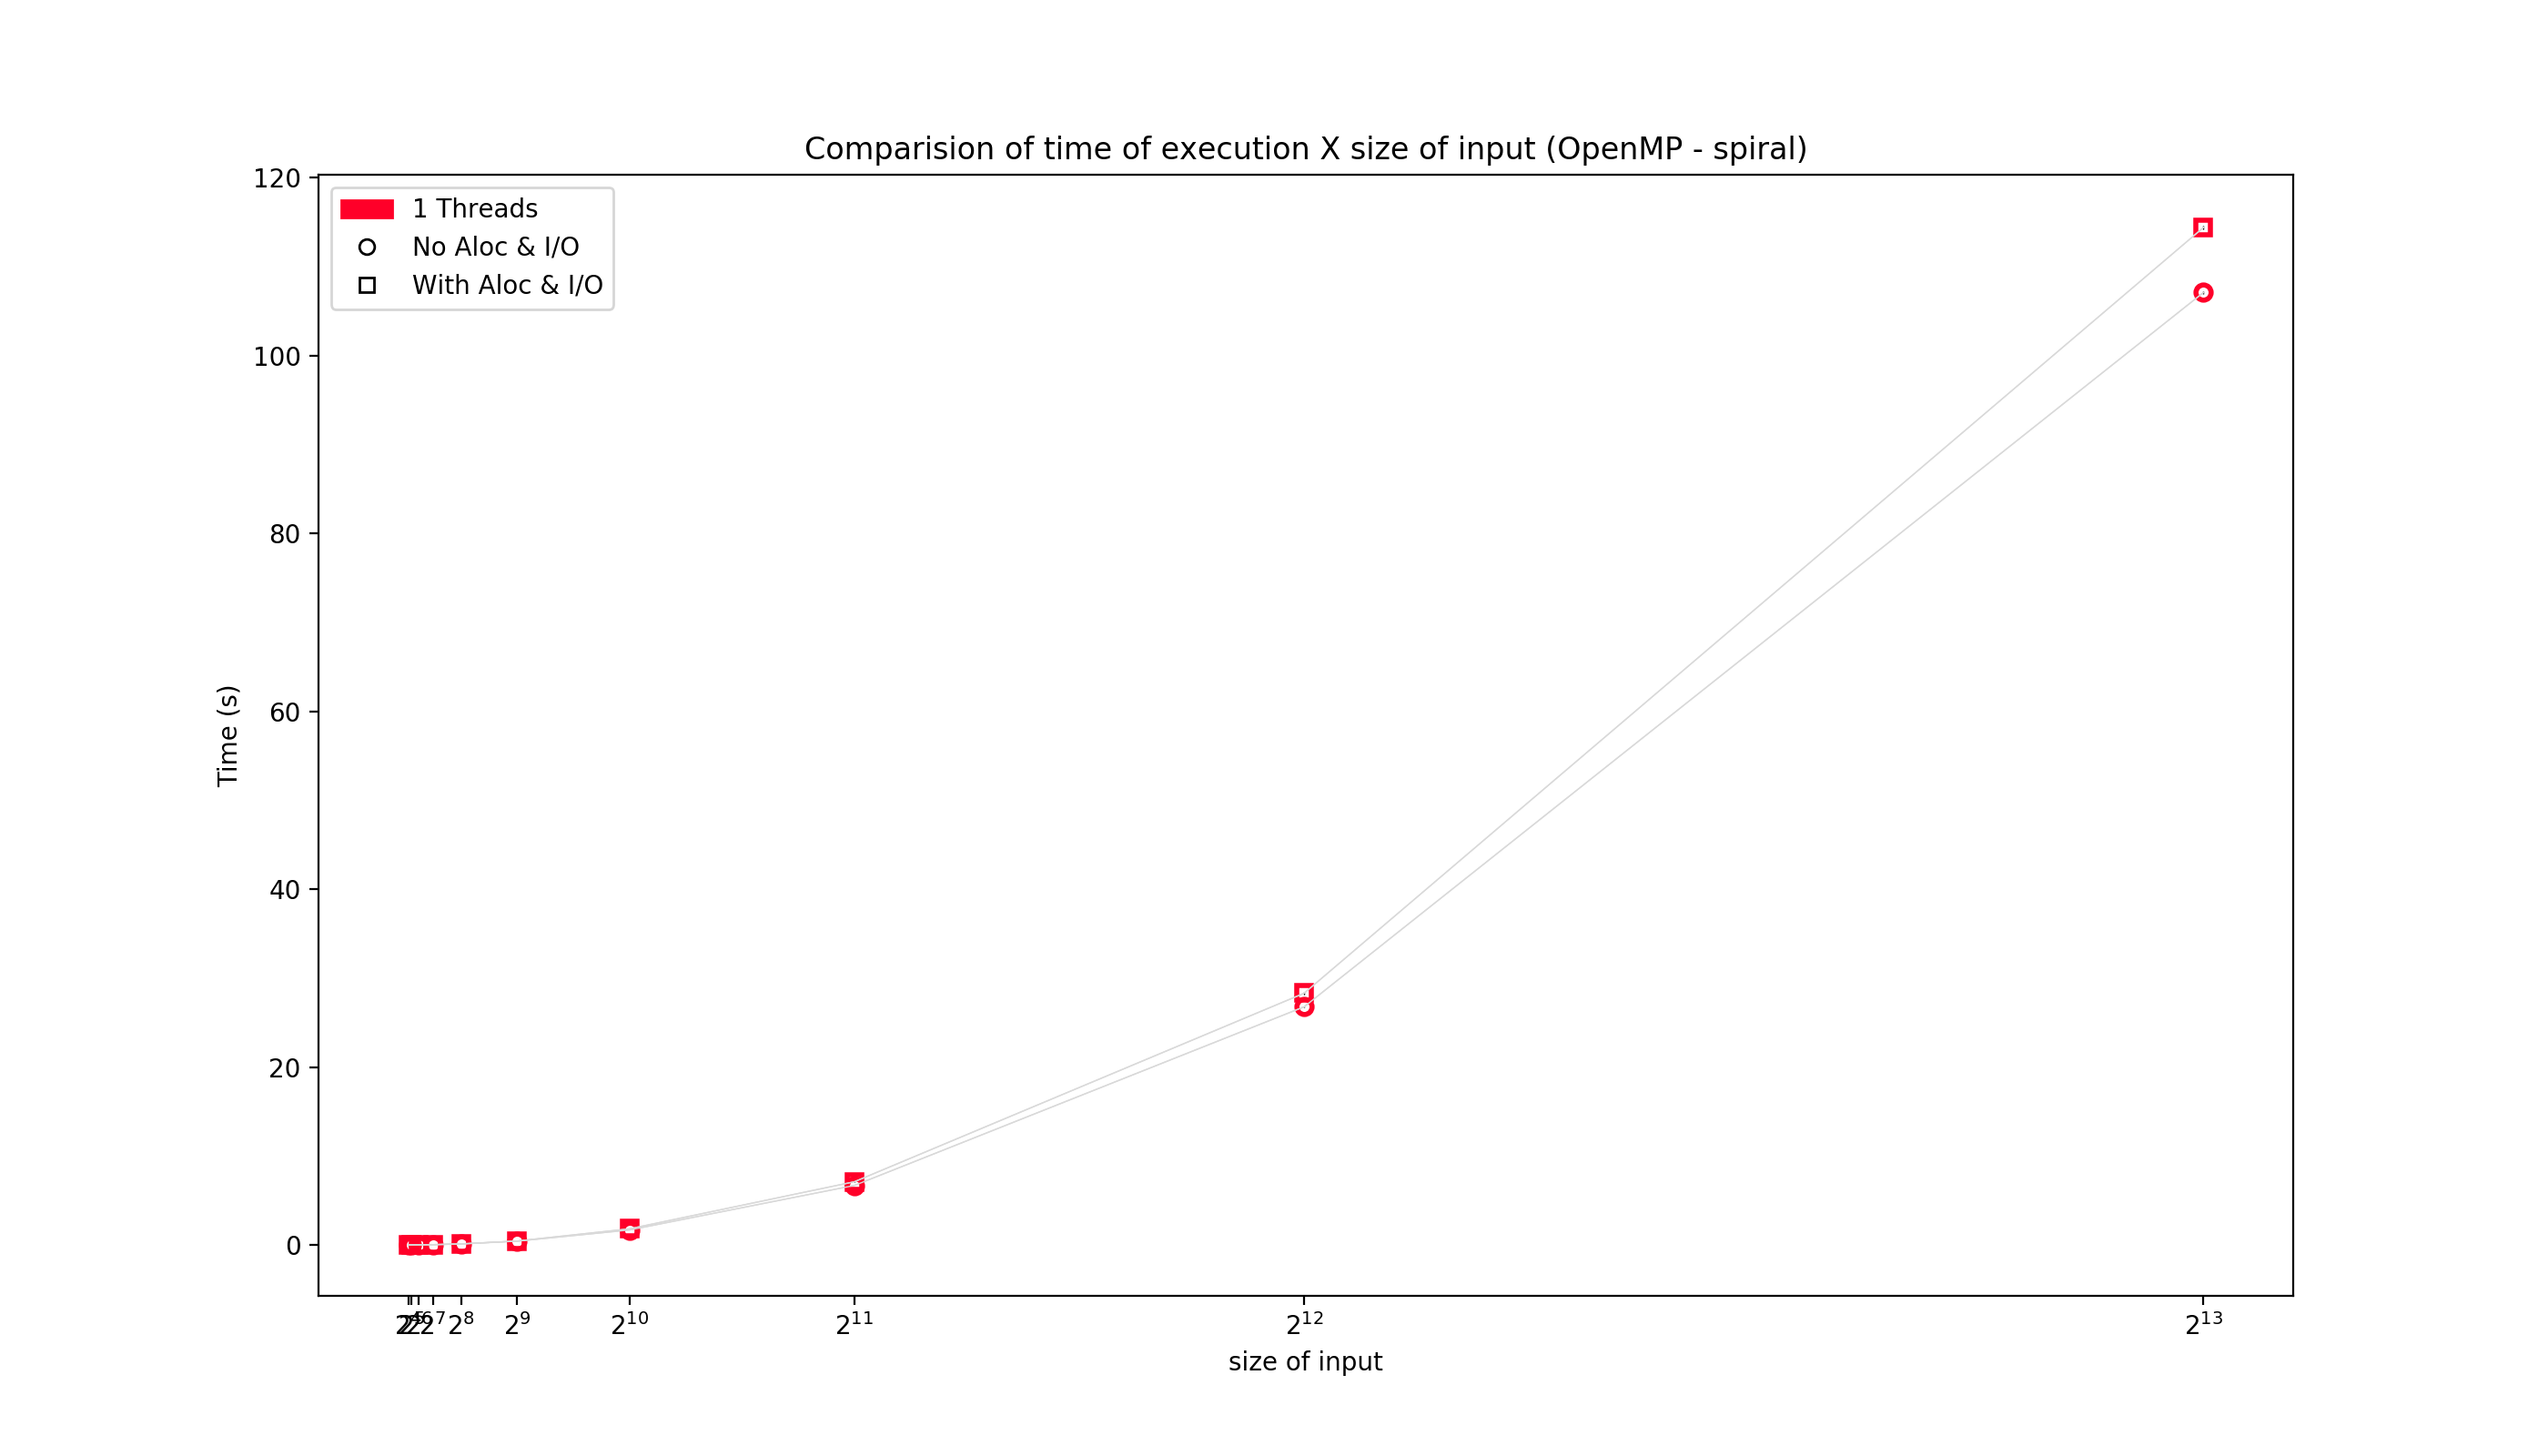
\includegraphics[scale=.50]{seq_comp/compare_timeXsize_spiral_OpenMPpng.png}}
\end{figure}

Nota-se que o tempo em cada região é diferente, pois em cada região pode haver mais cálculos de pontos com mais interações. Notemos ainda que a diferença de tempo para cada tamanho de entrada se mantem mesmo mudando-se as regiões. Por exemplo, a versão sem alocação dinamica e sem operações de leitura e escrita executa cerca de 10 segundos mais rapido que a versão com, dado a entrada de tamanho $2^(13)$, independente da região. Isso ocorre, pois comandos de leitura e escrita e alocação dinamica, dependem do tamanho da entrada e independem do número de interações do cálculo para determinado ponto.

Para cada implementação também vemos que o tempo para calcular a região Full foi bastante menor que para as demais regiões:

\begin{figure}[H]
    \makebox[\textwidth][c]{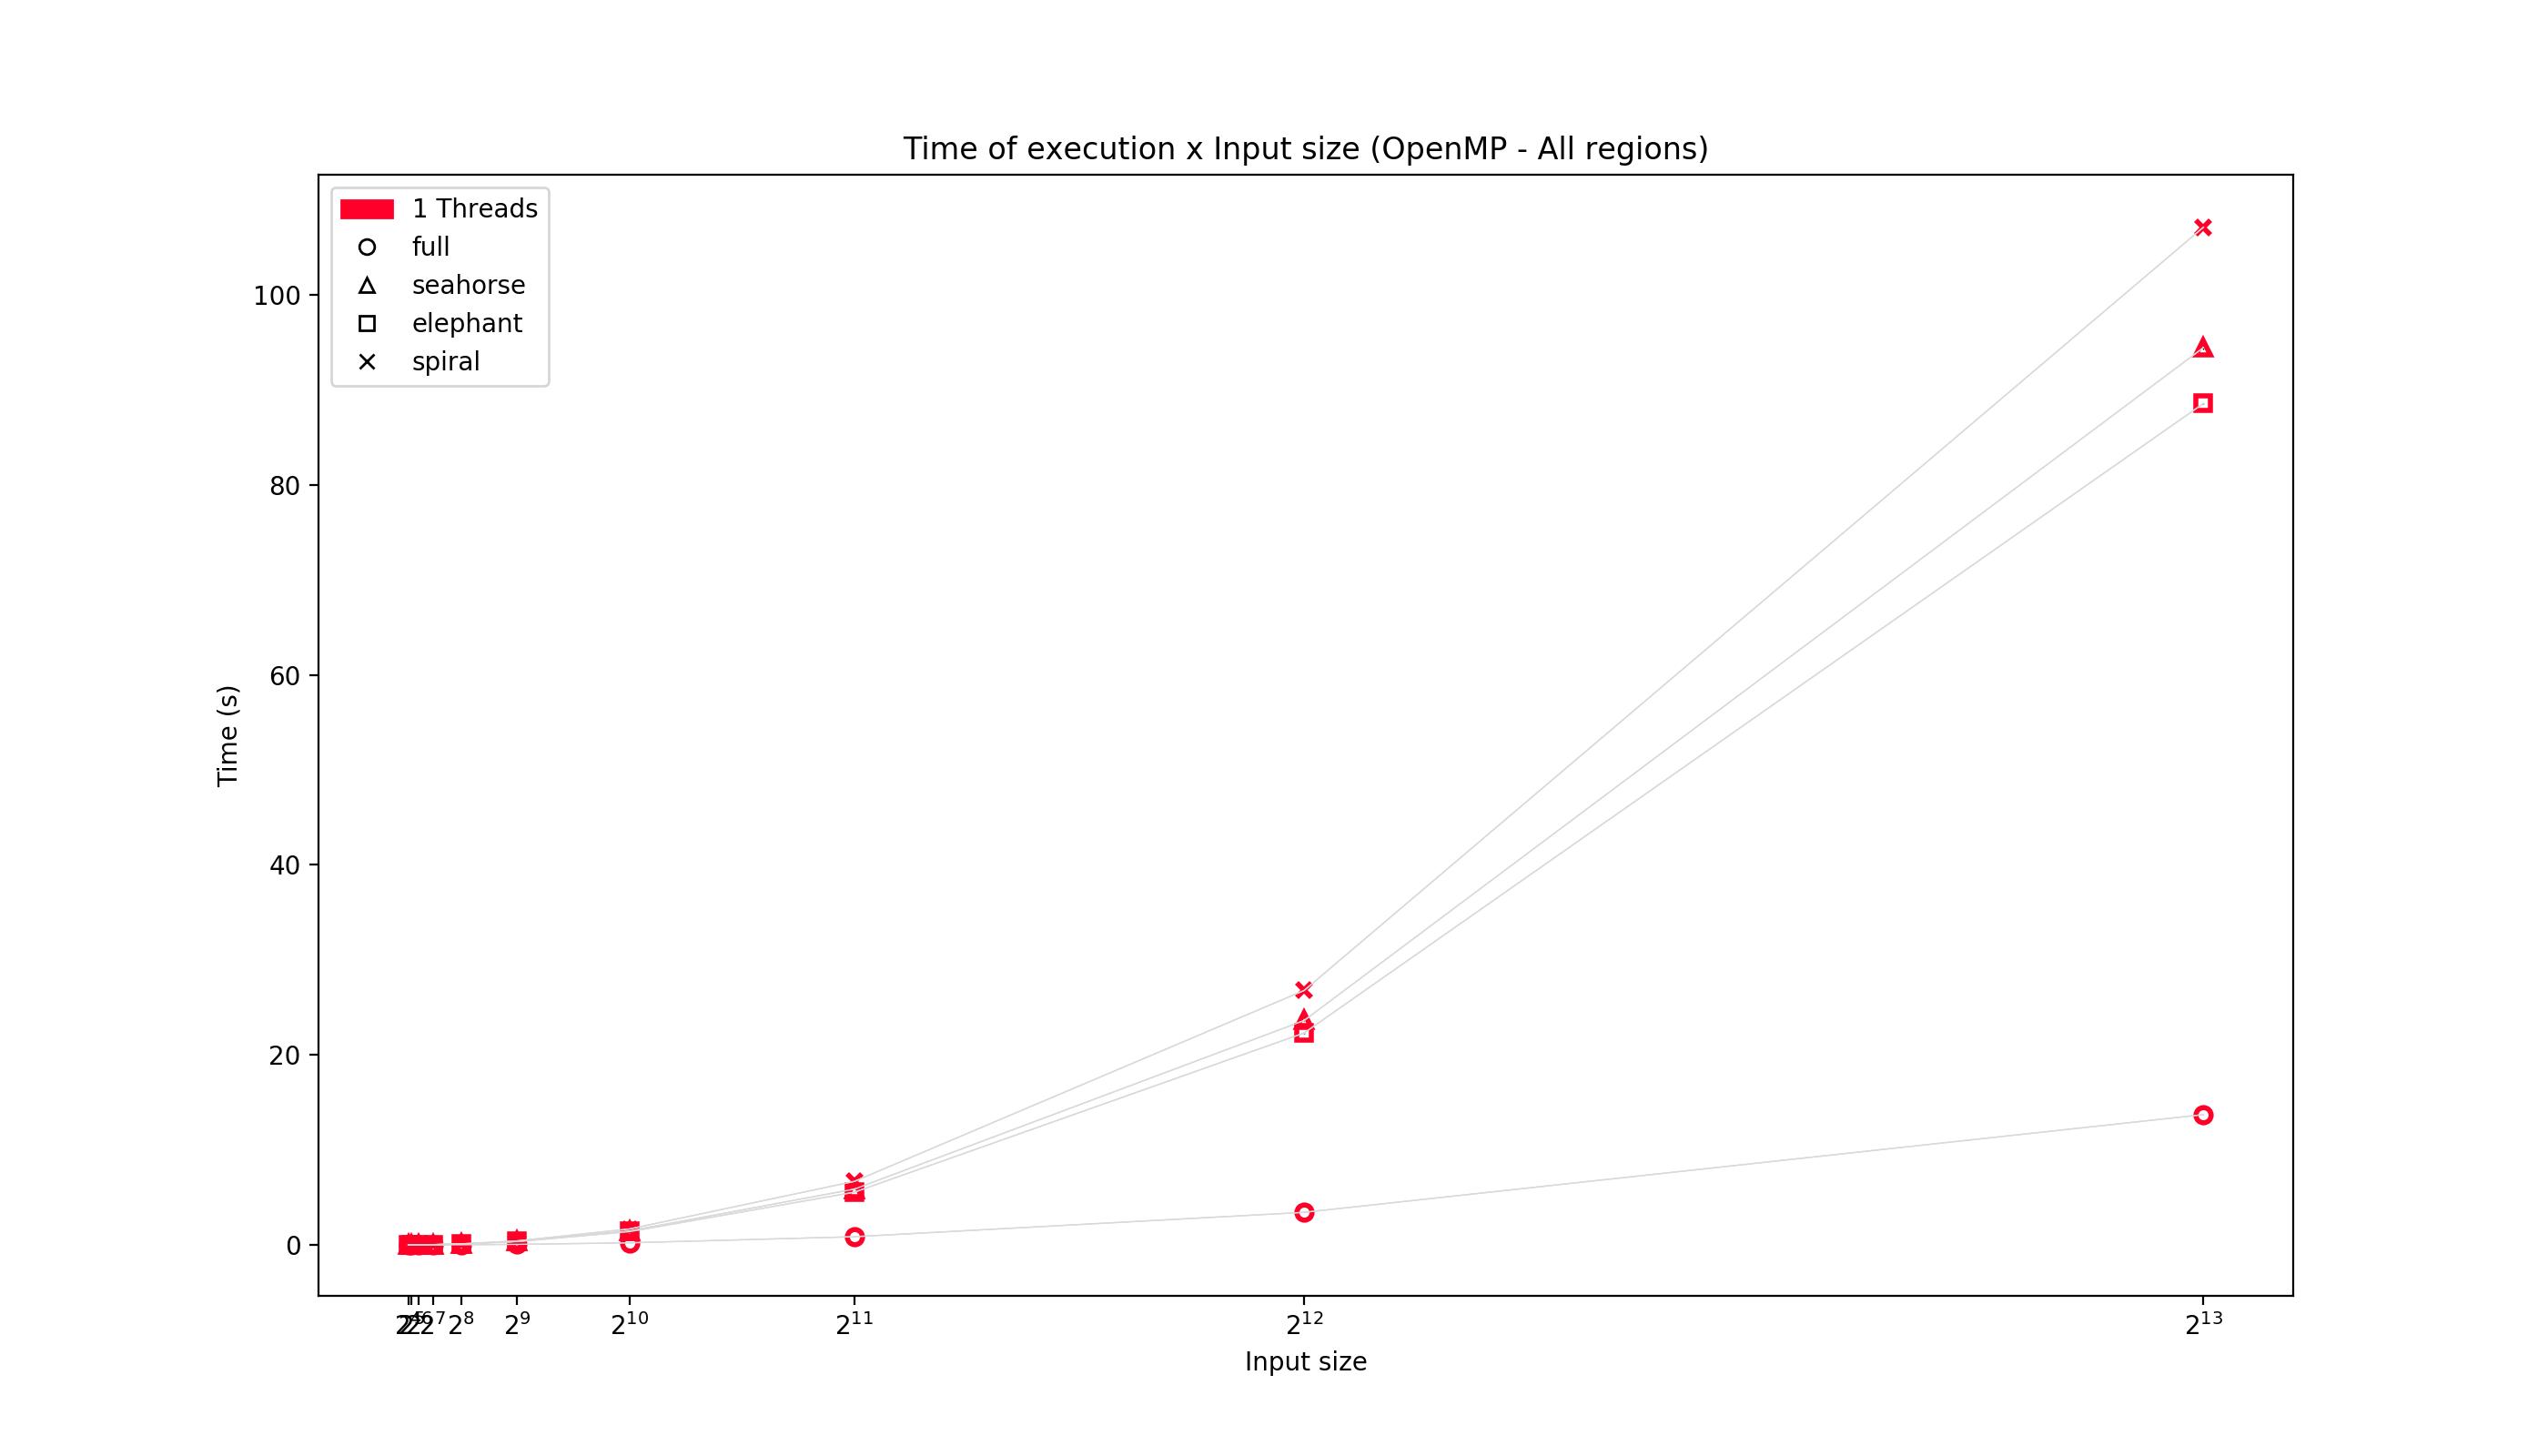
\includegraphics[scale=.50]{seq_no/all_timeXsize_OpenMPpng.png}}
\end{figure}

\begin{figure}[H]
    \makebox[\textwidth][c]{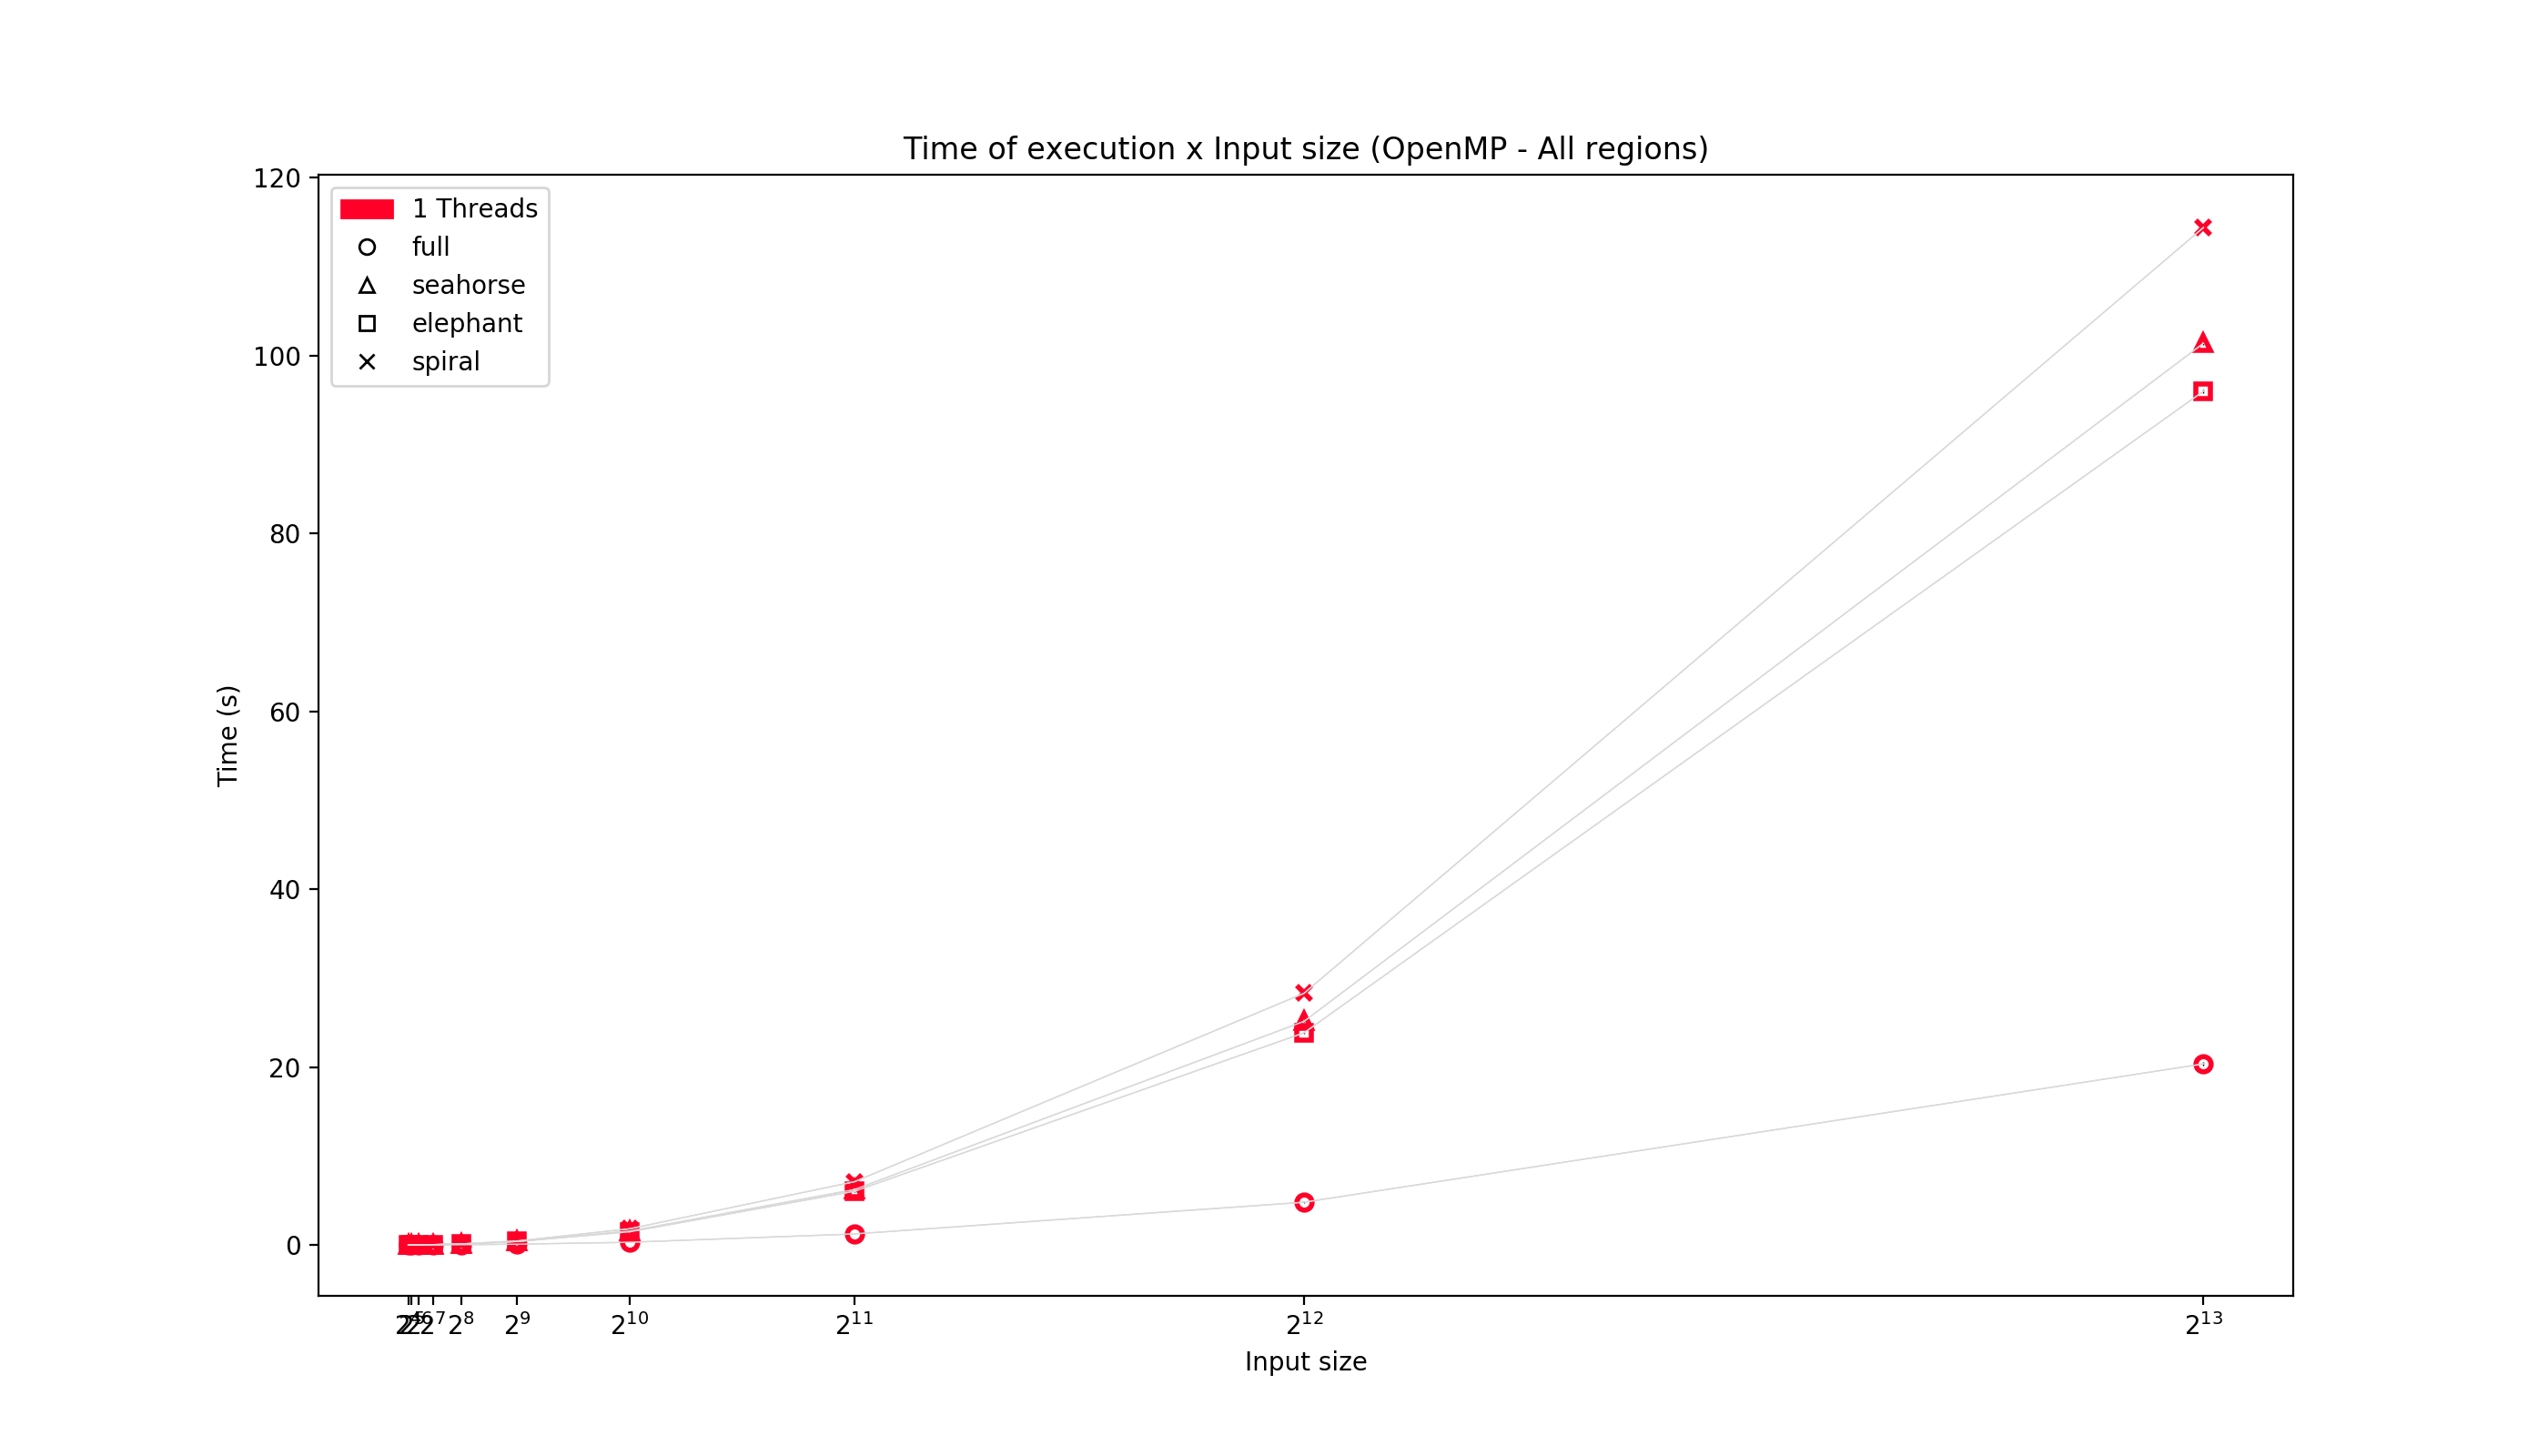
\includegraphics[scale=.50]{seq_with/all_timeXsize_OpenMPpng.png}}
\end{figure}

%%%%%%%%%%%%%%%%%%%%% PTHREADS %%%%%%%%%%%%%%%%%%%%%%%%%%%%%%
\newpage
\section{Código em Pthreads}
Utilizamos duas diferentes abordagens para paralelizar o código com
o uso de pthreads, tentando se aproximar ao comportamento do OpenMP e 
suas diretivas {\em omp parallel for schedule (dynamic)} e {\em omp 
parallel for schedule (static)}. As diferenças de funcionamento dos 
dois códigos está na maneira em que o trabalho é dividido e como ele é
distribuído para cada thread.

\subsection{Implementação com Divisão Estática}
Chamamos de implementação com divisão estática a versão do nosso 
código em pthreads no qual o trabalho é dividido em $n$ pedaços de mesmo 
tamanho, e cada pedaço é dado a uma thread. Chamamos essa implementação
de estática porque cada thread recebe apenas um bloco de trabalho,
pré-determinado pela divisão feita, que será processado do começo ao
fim (no escopo da thread) pela mesma thread.

Para implementar esse código, precisamos apenas construir uma estrutura
de dados que era capaz de guardar um bloco de pixels a ser calculado.
Dado essa estrutura, basta criar uma thread para cada bloco de trabalho,
que por sua vez deve calcular os pixels correspondentes e atualizar o 
buffer de cores.

Devemos observar que essa implementação pode implicar em threads ociosas
enquanto outras estão trabalhando. Como a quantidade de iterações
necessárias para se calcular o valor de um pixel varia, é possível que
um bloco de pixels seja calculado muito mais rápido do que outro; 
imagine por exemplo um bloco onde cada ponto calculado diverge 
rapidamente e outro bloco onde isso não acontece. Portanto, como a 
divisão de trabalho é estática, é provável que uma thread termine seu
trabalho muito antes de outra, o que significa em um uso não muito bom
de recursos da máquina.

Uma possível solução para esse problema seria o aumento no número de 
threads, o que cria uma fragmentação maior do trabalho. Essa 
fragmentação ameniza o problema anterior porque divide mais o trabalho,
deixando menor a diferença de tempo necessário para se calcular cada 
parte. Entretanto, criar um número excessivo de threads pode dar mais
trabalho ao escalonador do sistema operacional, que deve lidar com 
várias linhas de processamento.

\begin{figure}[!ht]
    \centering
    \begin{tabular}{c c}
        \subfigure[] {\scalebox{.35}{
            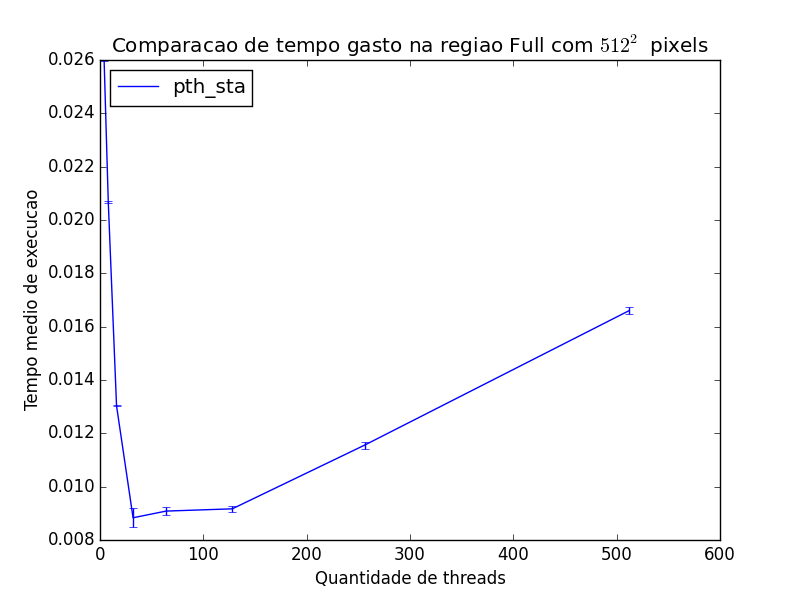
\includegraphics{pthread_numthreads/time_x_thread_numpth_sta_n512.png}}
            \label {fig:higher_thread_num:A}
        }
        &
        \subfigure[] {\scalebox{.35}{
            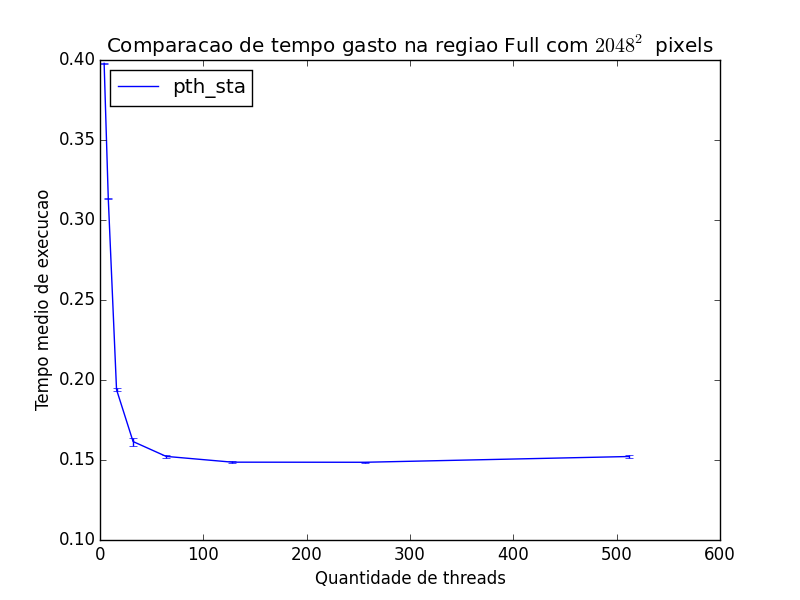
\includegraphics{pthread_numthreads/time_x_thread_numpth_sta_n2048.png}}
            \label {fig:higher_thread_num:B}
        }

    \end{tabular}
    \caption{É possível notar em ambas figuras que o aumento do número
    de threads de fato diminui o tempo de execução do programa. No 
    gráfico \ref{fig:higher_thread_num:A} fica evidente que o tempo 
    gasto no controle das threads pode afetar o tempo de execução do
    programa.}
    \label{fig:higher_thread_num} 
\end{figure}

\subsection{Implementação com Divisão Dinâmica}
A implementação dinâmica do nosso programa também divide o trabalho em
$n$ pedaços, entretanto agora $n$ não é mais, necessariamente o número
de threads disponíveis. Após dividir o trabalho em pedaços, o nosso 
programa agora é capaz de, dinamicamente, delegar blocos de pixels a 
cada thread. Portanto, agora diminuímos o problema de threads ociosas,
porque podemos dividir mais os blocos de trabalho e sempre que uma 
thread termina um bloco, podemos dar a ela um novo bloco para computar 
(desde que ainda haja trabalho a ser feito).

Veja abaixo um pseudo-código para esse programa:
\begin{algorithmic}[1]
\Function{ComputeMandelbrot}{}
    \State $S \gets $ lista de nacos de todos os pixels
    \While{$S \neq \emptyset$}
        \State $chunk \gets S$.popChunk ()
        \State Espere {\em alguma} thread estar livre
        \ForAll{Threat $T$}
            \If{$T$ está livre}
                \State $T$.compute ($chunk$)
            \EndIf
        \EndFor
    \EndWhile 
    \EndFunction
\end{algorithmic}

A implementação desse código é um pouco mais complicada, porque depende,
além da estrutura de dados já usada na implementação estática, de um 
maior controle de concorrência. O conceito principal utilizado é o de 
{\em condition variable}, que nos permite colocar a linha principal de
execução em espera, enquanto as threads calculam os pixels, para voltar
a ser executada quando alguma thread estiver livre.

\begin{figure}[!ht]
    \centering
    \begin{tabular}{c c}
        \subfigure[] {\scalebox{.35}{
            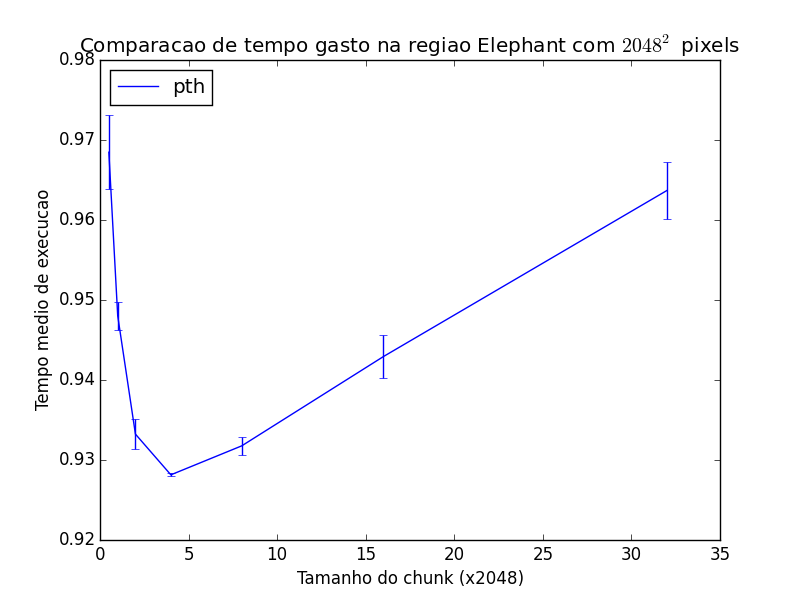
\includegraphics{pthread_chunk/time_x_chunk_sizepth2048elephant.png}}
            \label {fig:pthreads_chunk_size:A}
        }
        &
        \subfigure[] {\scalebox{.35}{
            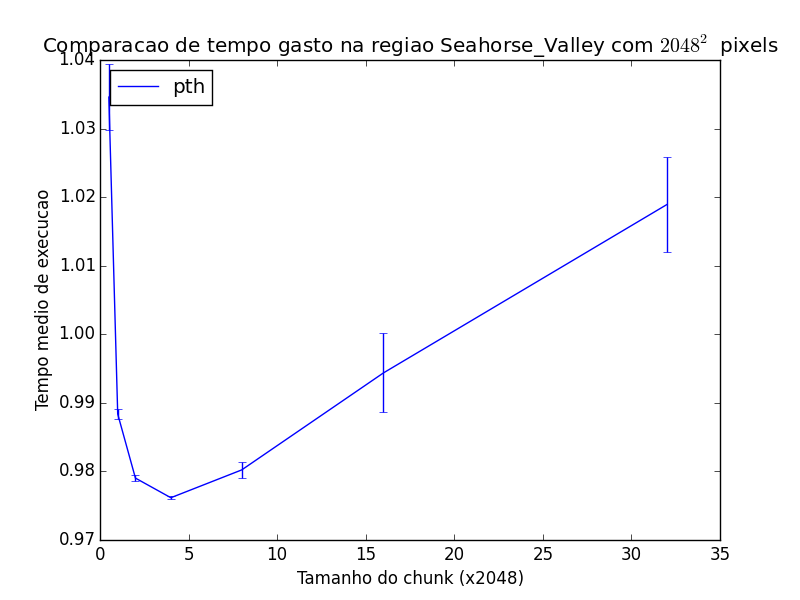
\includegraphics{pthread_chunk/time_x_chunk_sizepth2048seahorse_valley.png}
        }
            \label {fig:pthreads_chunk_size:B}
        }
        \\
        \subfigure[] {\scalebox{.35}{
            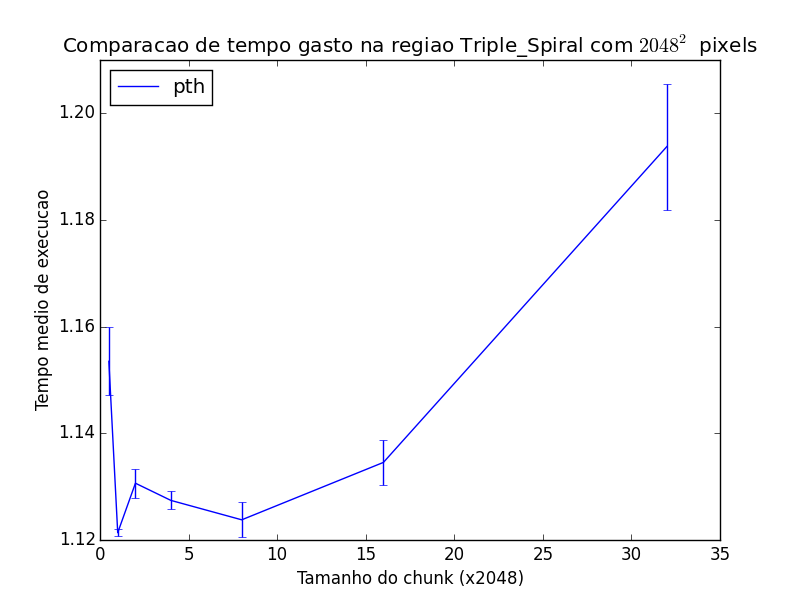
\includegraphics{pthread_chunk/time_x_chunk_sizepth2048triple_spiral.png}}
            \label {fig:pthreads_chunk_size:C}
        }
        &
        \subfigure[] {\scalebox{.35}{
            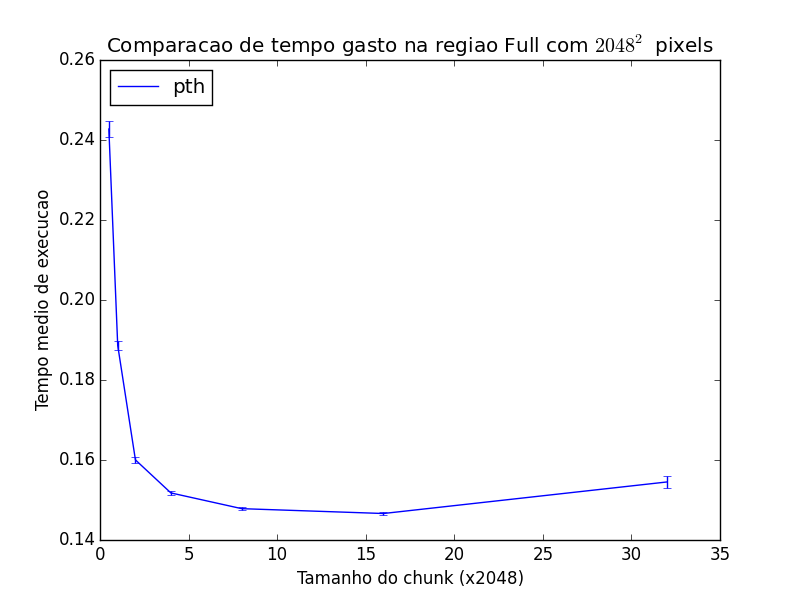
\includegraphics{pthread_chunk/time_x_chunk_sizepth2048full.png}}
            \label {fig:pthreads_chunk_size:D}
        }
        
    \end{tabular}
    \caption{Verificamos empiricamente que definir o tamanho do chunk 
        como  o tamanho do lado da imagem traz bons resultados para o
        tempo de execução.}
    \label{fig:pthreads_chunk_size} 
\end{figure}


Diminuído o problema de threads ociosas, é esperado que essa 
implementação seja mais rápida do que a anterior, porém, é necessário 
notar que o nosso código ficou mais complexo, e exige mais recursos
computacionais para o controle das threads. Esse tempo pode ser 
prejudicial se o tamanho do chunk for pequeno, pois nessa situação
há muitas trocas de chunks em cada thread, fazendo com que a maior parte
do tempo de processamento seja gasto no controle das threads. Por outro
lado, se temos chunks muito grandes, o tempo gasto deve aumentar, porque
caímos novamente no problema da implementação static, onde o trabalho 
não era bem dividido. Depois de fazer alguns testes, verificamos 
que definir o tamanho do chunk igual a quantidade de pixels em uma linha
da imagem nos dava bons resultados; inclusive, esse foi o mesmo valor 
adotado em nossa implementação com OpenMP.

\begin{figure}[!h]
    \centering
    \begin{tabular}{c c}
        \subfigure[] {\scalebox{.35}{
            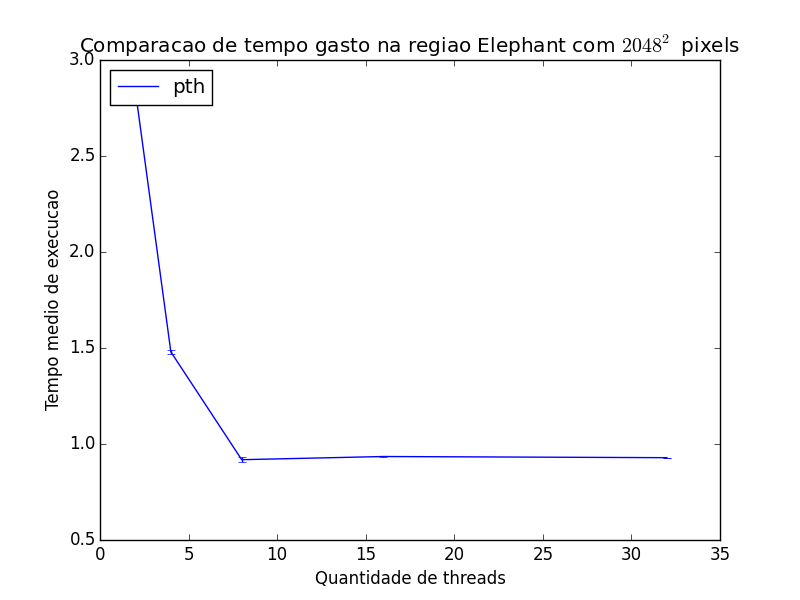
\includegraphics{pthread_numthreads/time_x_thread_numpth2048_elephant.png}}
            \label {fig:pthreads_num_threads:A}
        }
        &
        \subfigure[] {\scalebox{.35}{
        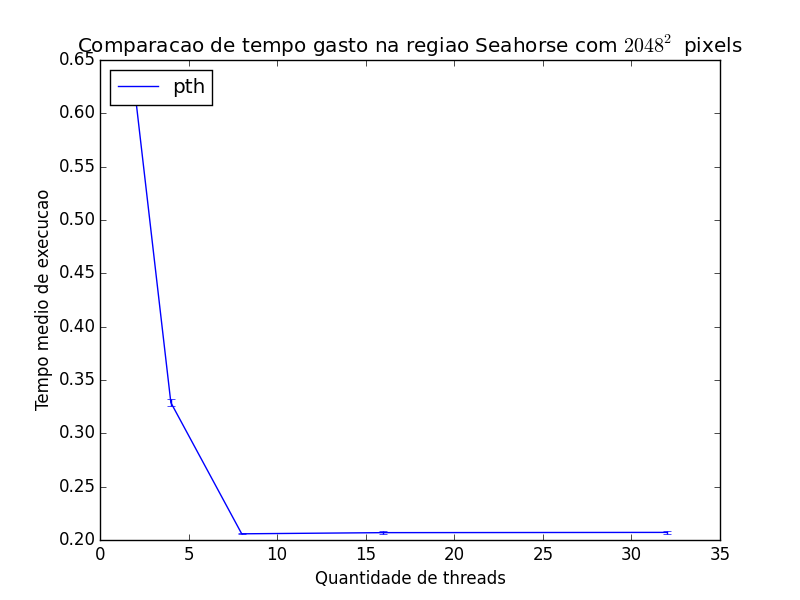
\includegraphics{pthread_numthreads/time_x_thread_numpth2048_seahorse.png}
        }
            \label {fig:pthreads_num_threads:B}
        }
        \\
        \subfigure[] {\scalebox{.35}{
            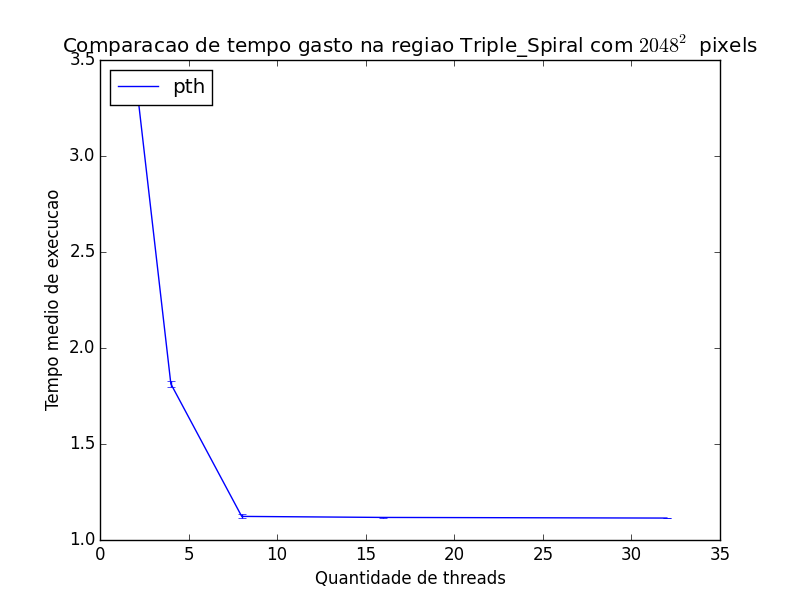
\includegraphics{pthread_numthreads/time_x_thread_numpth2048_triple_spiral.png}}
            \label {fig:pthreads_num_threads:C}
        }
        &
        \subfigure[] {\scalebox{.35}{
            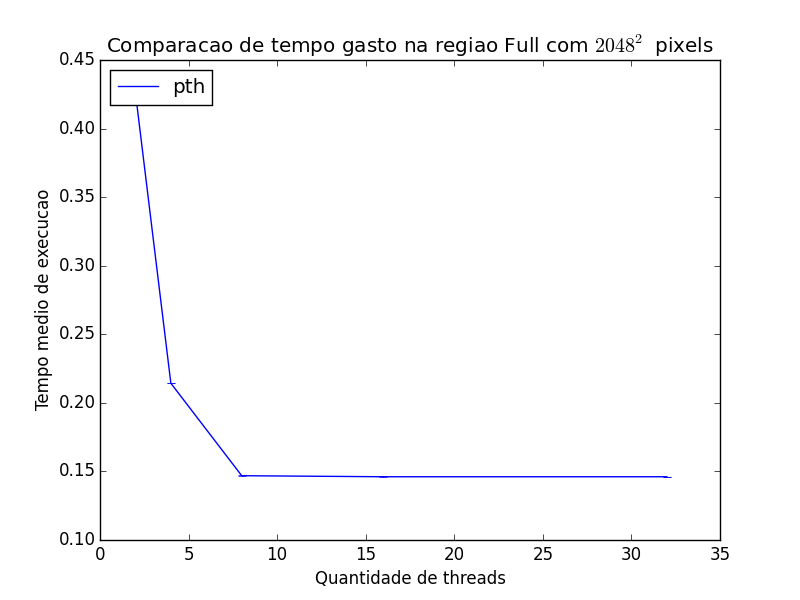
\includegraphics{pthread_numthreads/time_x_thread_numpth2048_full.png}}
            \label {fig:pthreads_num_threads:D}
        }
        
    \end{tabular}
    \caption{Podemos observar que existe uma saturação de melhora de 
    desempenho quando o número de threads atinge o número de cores (8)
    da máquina.}
    \label{fig:pthreads_thread_num} 
\end{figure}

Como distribuímos dinamicamente os blocos de trabalho, é esperado que
o aumento do número de threads não melhore o problema de threads 
ociosas, diferente do que vimos na implementação com divisão estática
e na figura \ref{fig:higher_thread_num}. A melhora com o aumento de 
threads deve vir unicamente do melhor uso da quantidade de cores da 
máquina, ou seja, a quantidade de threads deve melhorar o desempenho 
enquanto não foi maior do que o número de processadores da máquina.
De fato, observamos esse comportamento na figura 
\ref{fig:pthreads_thread_num}

Veja abaixo a comparação em consumo de tempo entre as duas 
implementações de paralelismo com Pthreads:
\begin{figure}[!h]
    \centering
    \begin{tabular}{c c}
        \subfigure[] {\scalebox{.35}{
            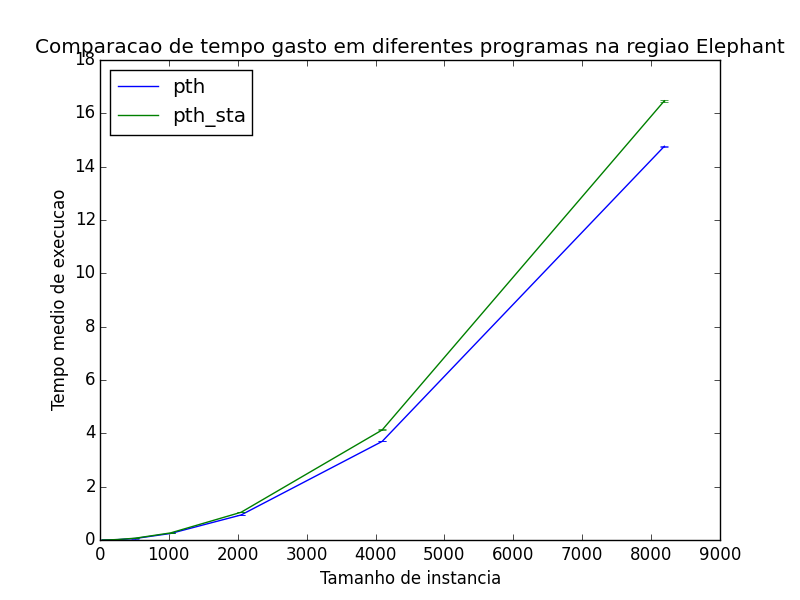
\includegraphics{pthread_din_sta/time_x_sizepth-pth_staelephant.png}}
            \label {fig:pthreads_din_sta:A}
        }
        &
        \subfigure[] {\scalebox{.35}{
        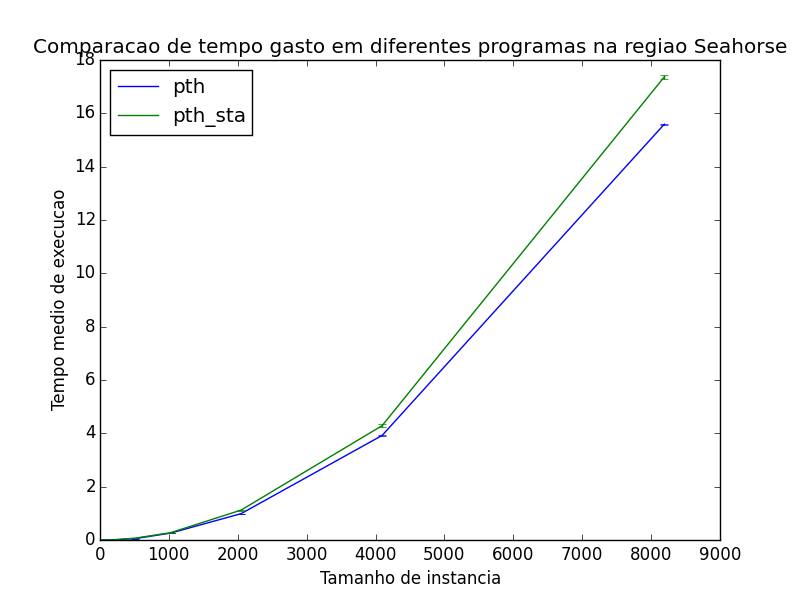
\includegraphics{pthread_din_sta/time_x_sizepth-pth_staseahorse.png}
        }
            \label {fig:pthreads_din_sta:B}
        }
        \\
        \subfigure[] {\scalebox{.35}{
            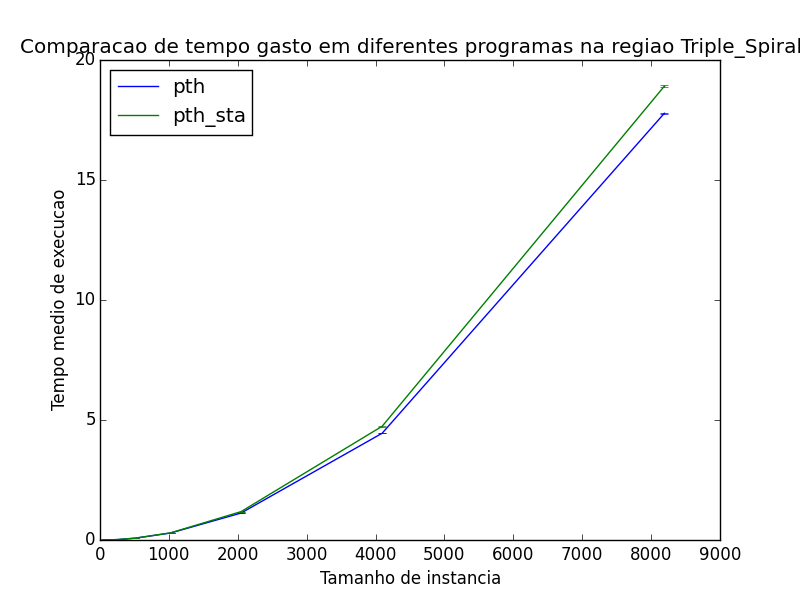
\includegraphics{pthread_din_sta/time_x_sizepth-pth_statriple_spiral.png}}
            \label {fig:pthreads_din_sta:C}
        }
        &
        \subfigure[] {\scalebox{.35}{
            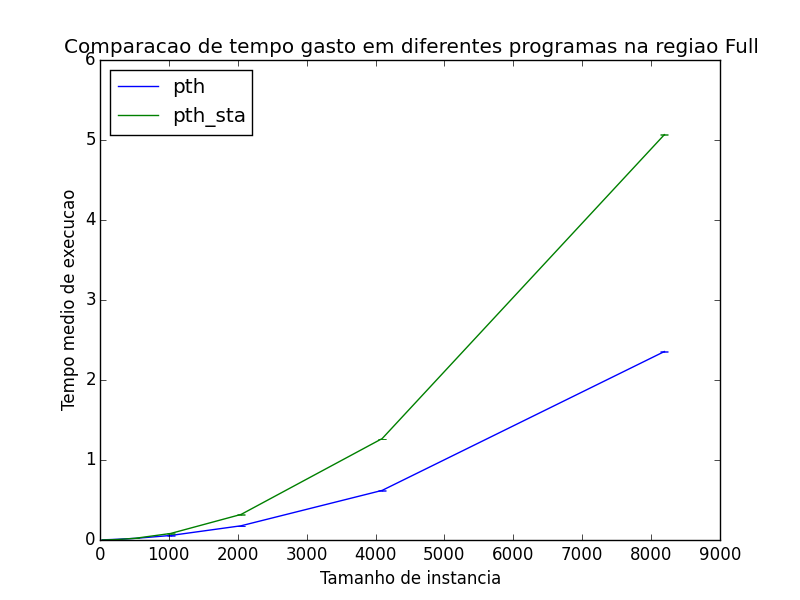
\includegraphics{pthread_din_sta/time_x_sizepth-pth_stafull.png}}
            \label {fig:pthreads_din_sta:D}
        }
        
    \end{tabular}
    \caption{Podemos observar nessas figuras que a implementação com
    divisão dinâmica possui desempenho melhor do que estático e que, 
    além disso, essa diferença tende a aumentar quando o tamanho da
    instância também aumenta. É provavel que as regiões onde o trabalho
    está 
    Esses testes foram realizados com número de threads igual
    a quantidade de processadores da máquina.}
    \label{fig:pthreads_din_sta} 
\end{figure}

%%%%%%%%%%%%%%%%%%%%% OPENMP %%%%%%%%%%%%%%%%%%%%%%%%%%%%%%
\newpage
\section{Código em OpenMP}
Para implementar a versão OpenMP do programa do cálculo do conjunto de Mandelbrot tivemos que remover a alocação de memória e comandos de leitura e escrita do códgio fornecido previamente.
Como não há comandos de leitura, os comandos de leitura e escrita são retirados, removendo-se a função \code{write\_to\_file()}. No caso de alocação de memória pode ser que o tempo de acesso a um vetor possa ser relevante, portanto não simplesmente removemos a função de alocação de memória. Para retirar as alocações, supomos que o tamanho máximo de uma imagem será de 11500px x 11500px e assim substituimos a alocação dinâmica do \code{image\_buffer} por uma alocação estática: \code{char image\_buffer[11500*11500][3]}.

Para paralelizar o cálculo, como esperado do OpenMP, é tão fácil como adicionar um \code{\#pragma} antes do \code{for} que realiza o cálculo para cada pixel da imagem:
\begin{lstlisting}[style=CStyle]
    #pragma omp parallel for private(...) num_threads(nThreads) schedule(dynamic)
    for (i_y = 0; i_y < i_y_max; i_y++) {
        c_y = c_y_min + i_y * pixel_height;
        ...
\end{lstlisting}

Implementando dessa forma obtemos os seguintes resultados:
\begin{figure}[H]
    \makebox[\textwidth][c]{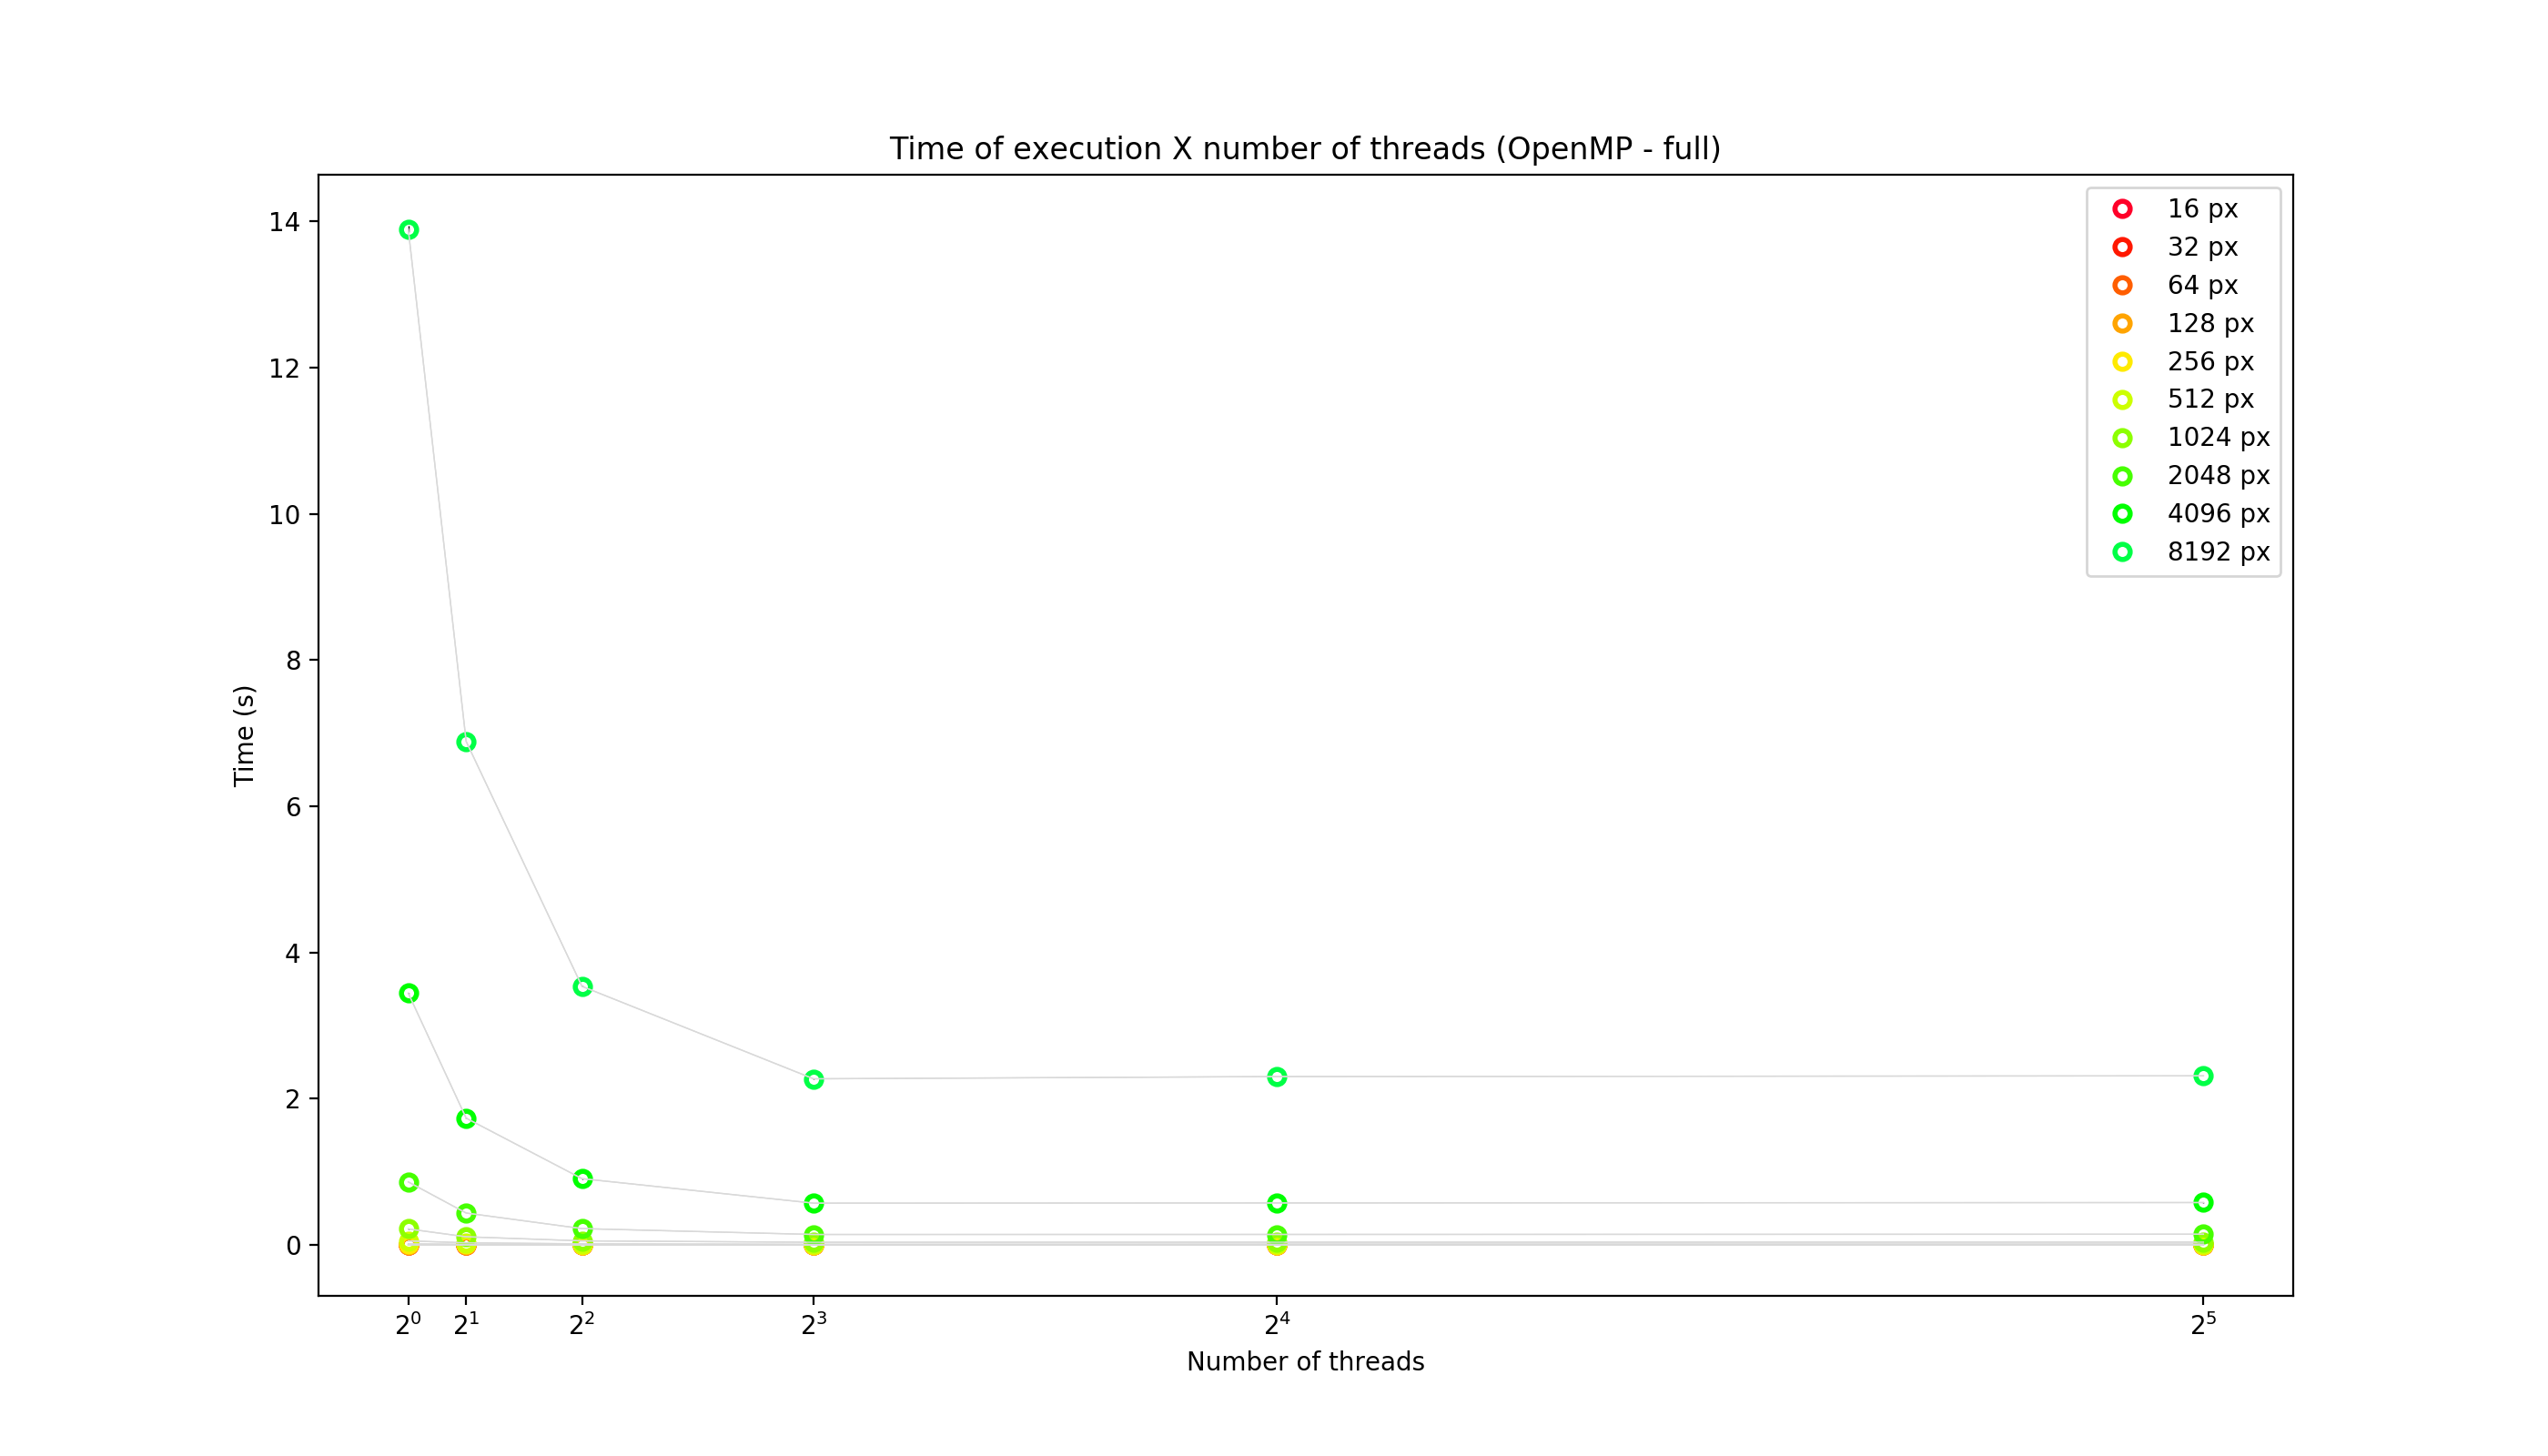
\includegraphics[scale=.60]{for_duplo_plot/timeXthread_full_OpenMPpng.png}}
    \caption{Esse gráfico mostra o tempo de execução X numero de threads para cada tamanho de entrada. Esses valores foram experimentados na região "full". Barras de erro também estão plotadas, porém são tão pequenas que talvez não estejam viziveis.}
\end{figure}

Percebemos que o aumento de threads de fato melhorou o tempo de execução do programa. No entanto ao ultrapassar 8, o mesmo número de cores da maquina testada, não houve grande melhora no tempo de execução. Esse mesmo comportamento foi observado para as demais regiões:

\begin{figure}[H]
    \makebox[\textwidth][c]{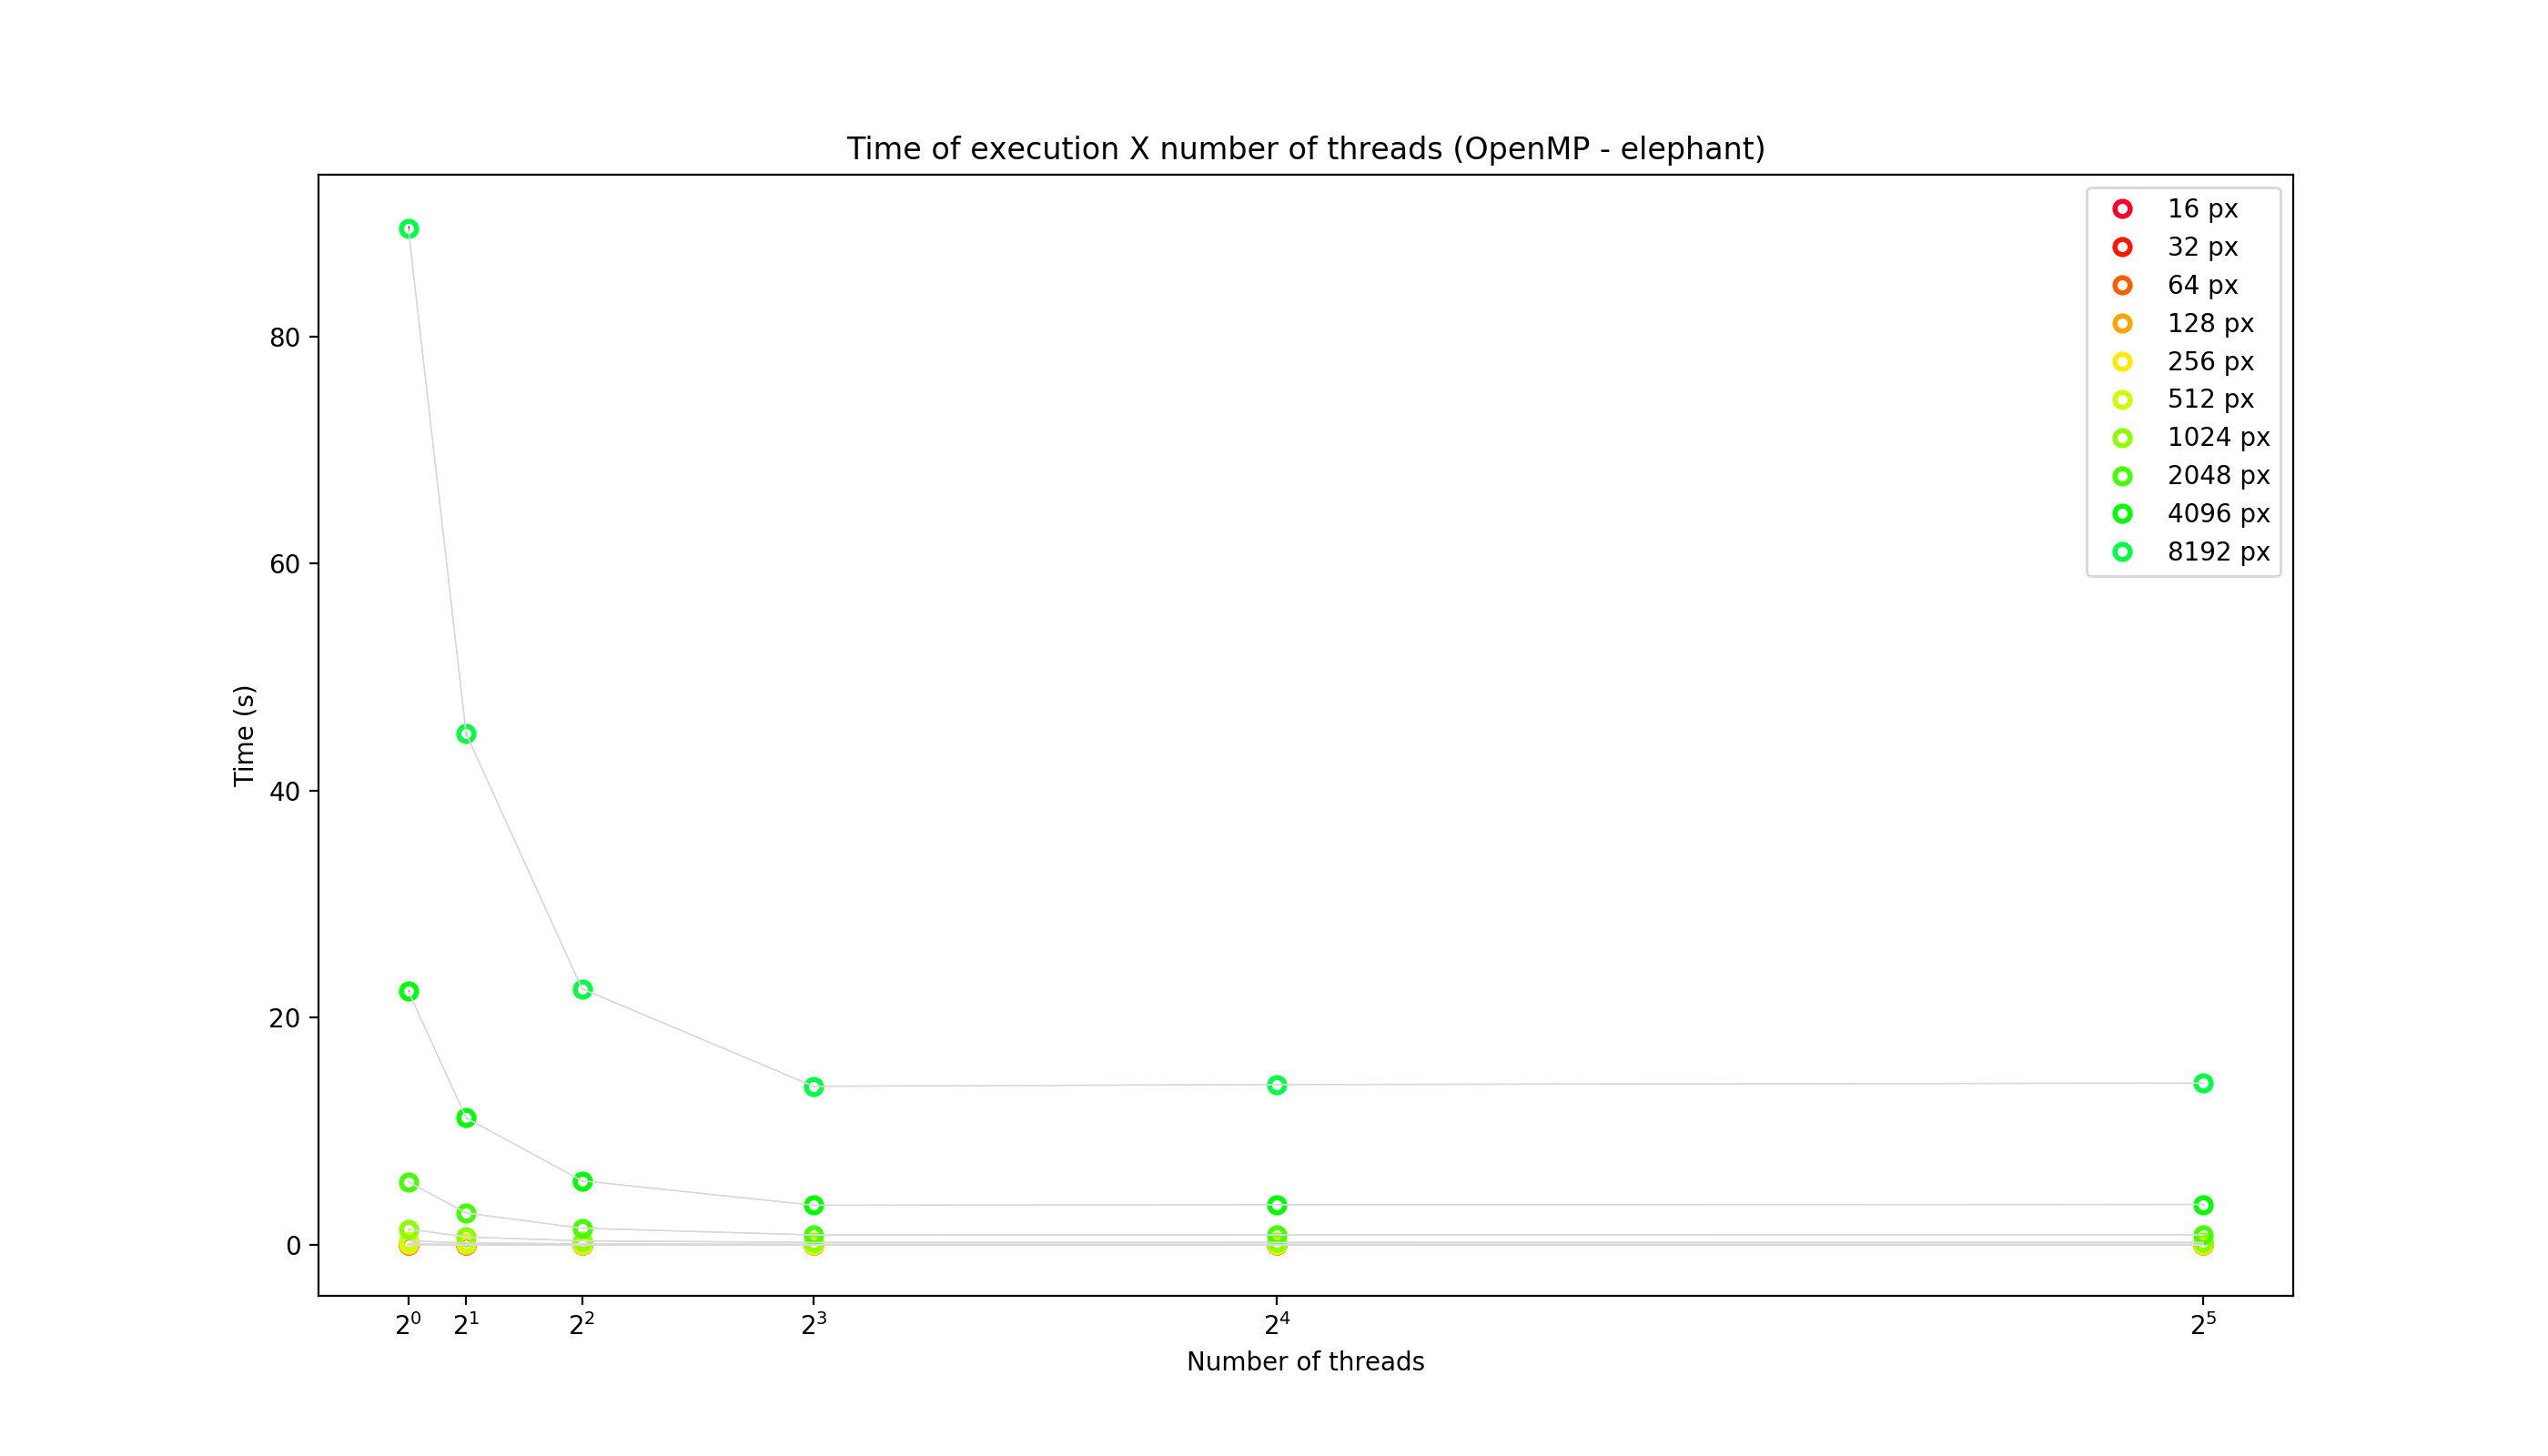
\includegraphics[scale=.50]{for_duplo_plot/timeXthread_elephant_OpenMPpng.png}}
\end{figure}

\begin{figure}[H]
    \makebox[\textwidth][c]{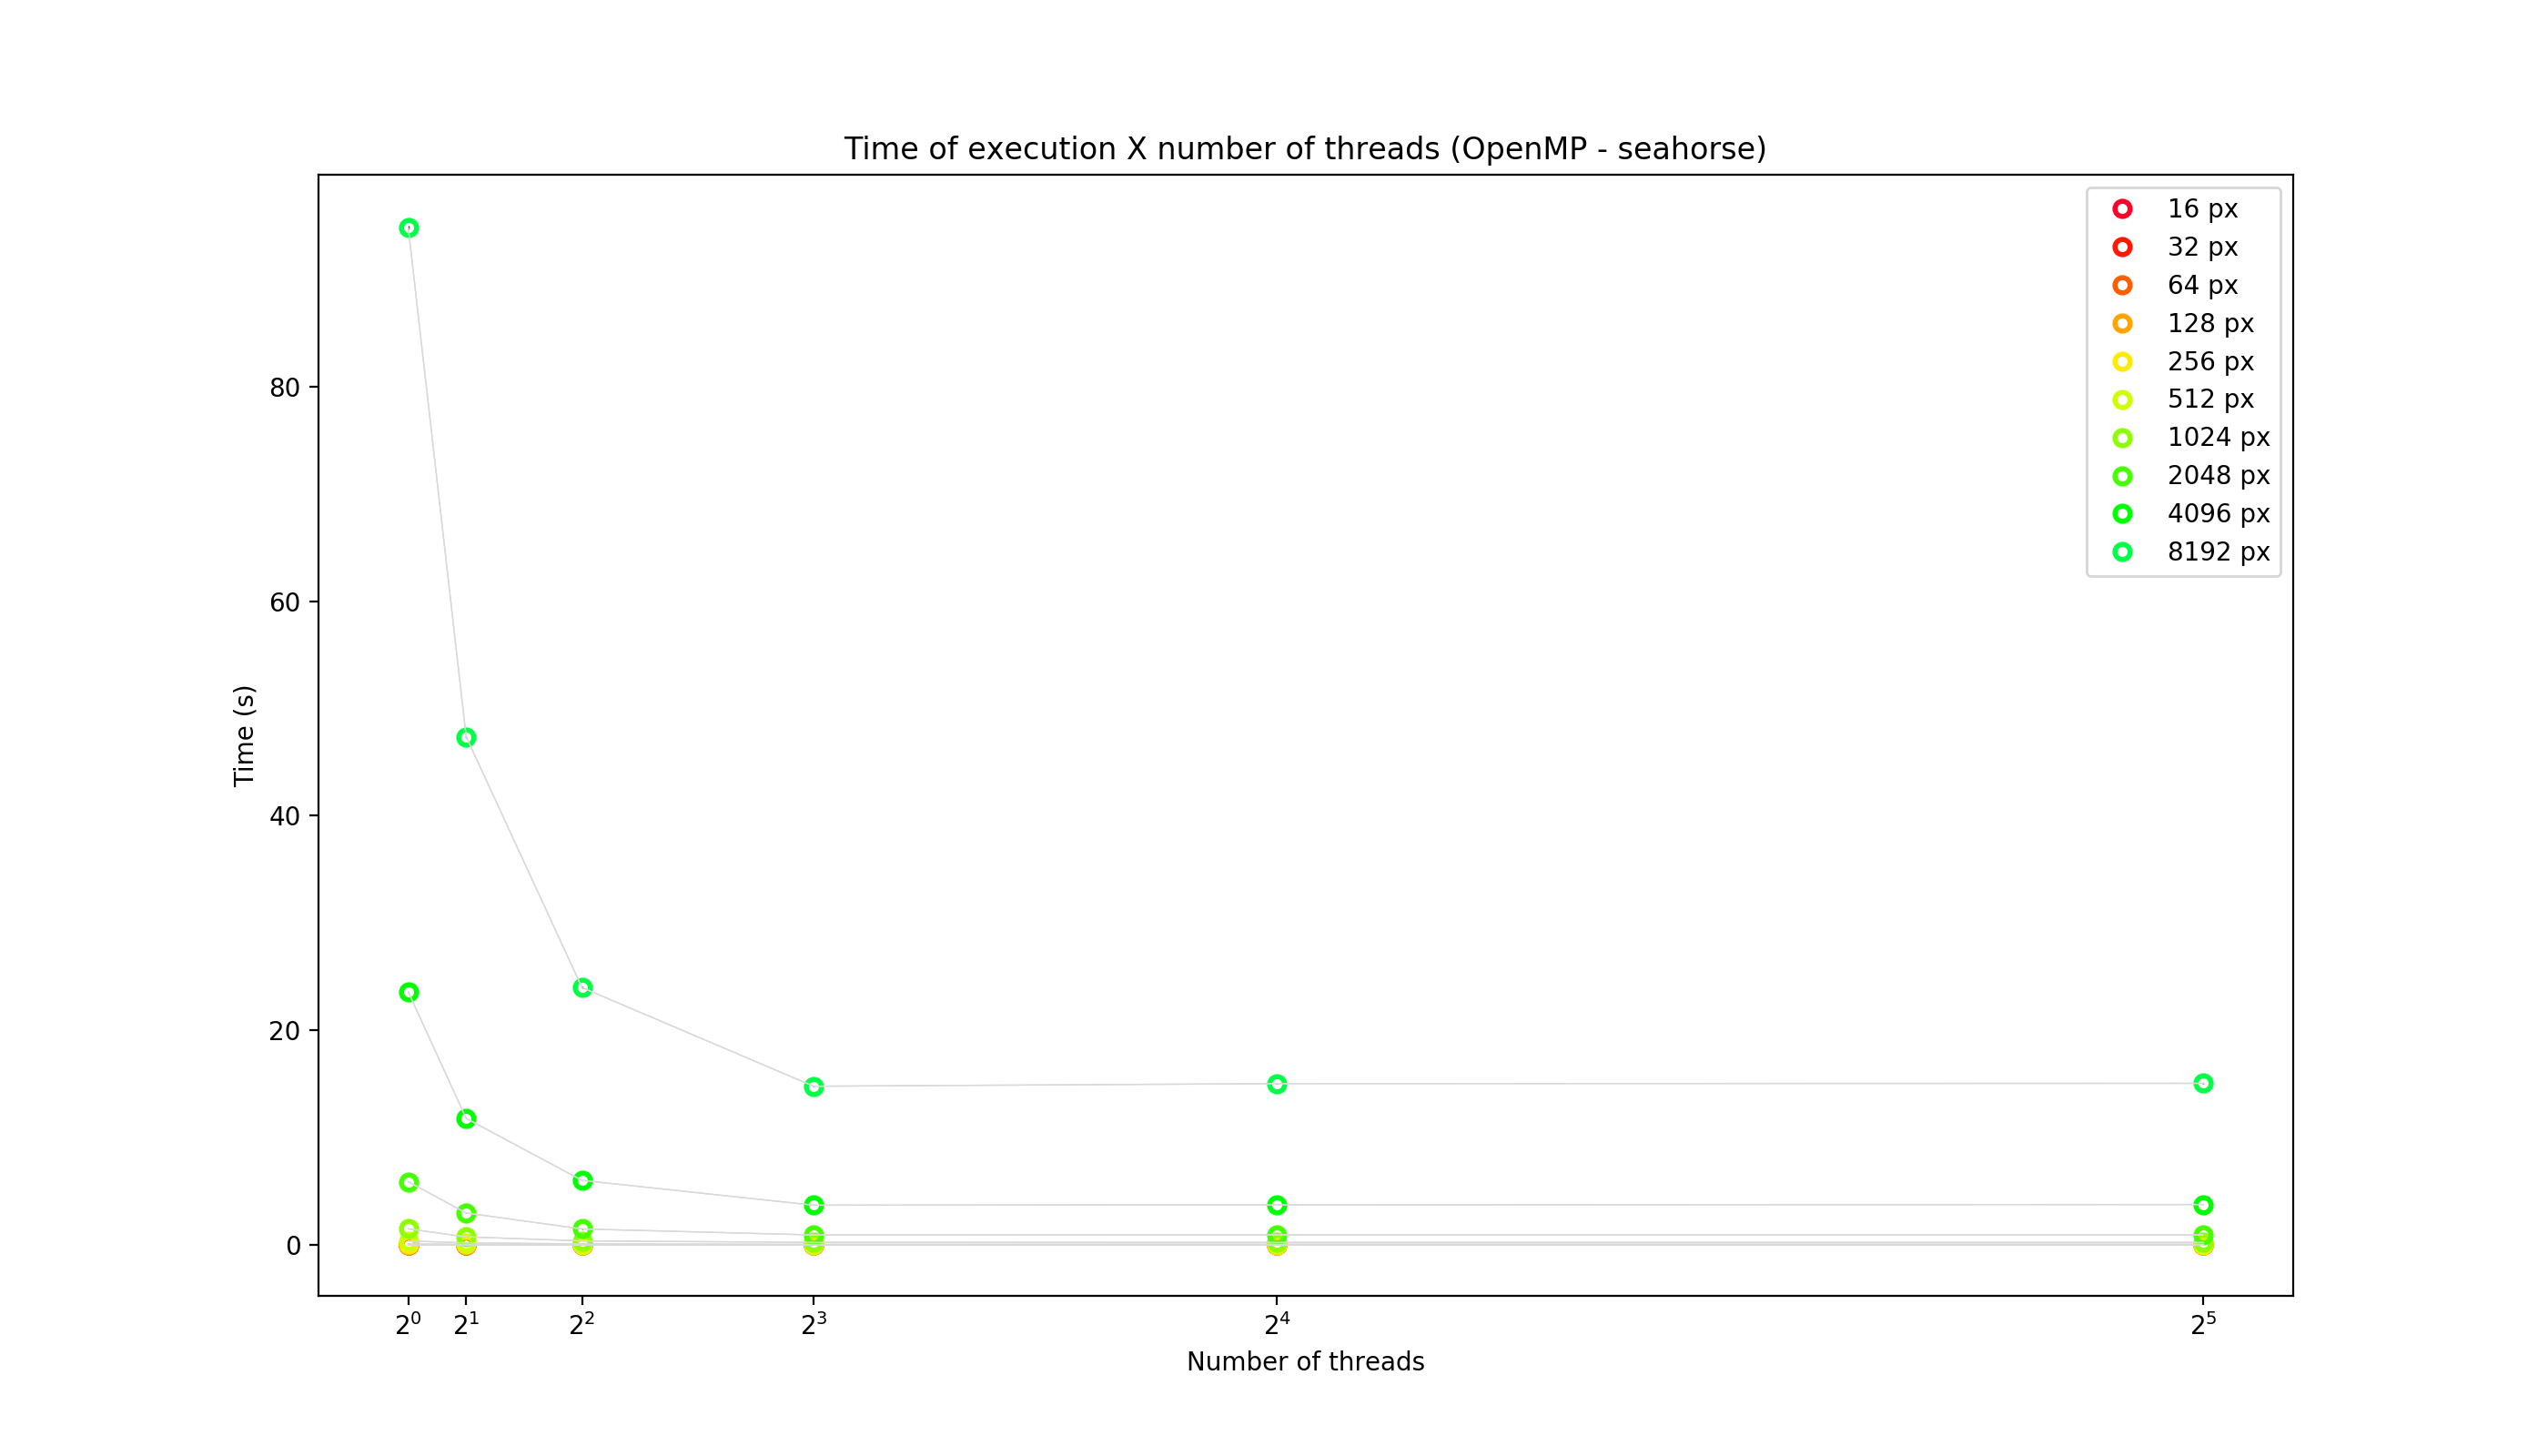
\includegraphics[scale=.50]{for_duplo_plot/timeXthread_seahorse_OpenMPpng.png}}
\end{figure}

\begin{figure}[H]
    \makebox[\textwidth][c]{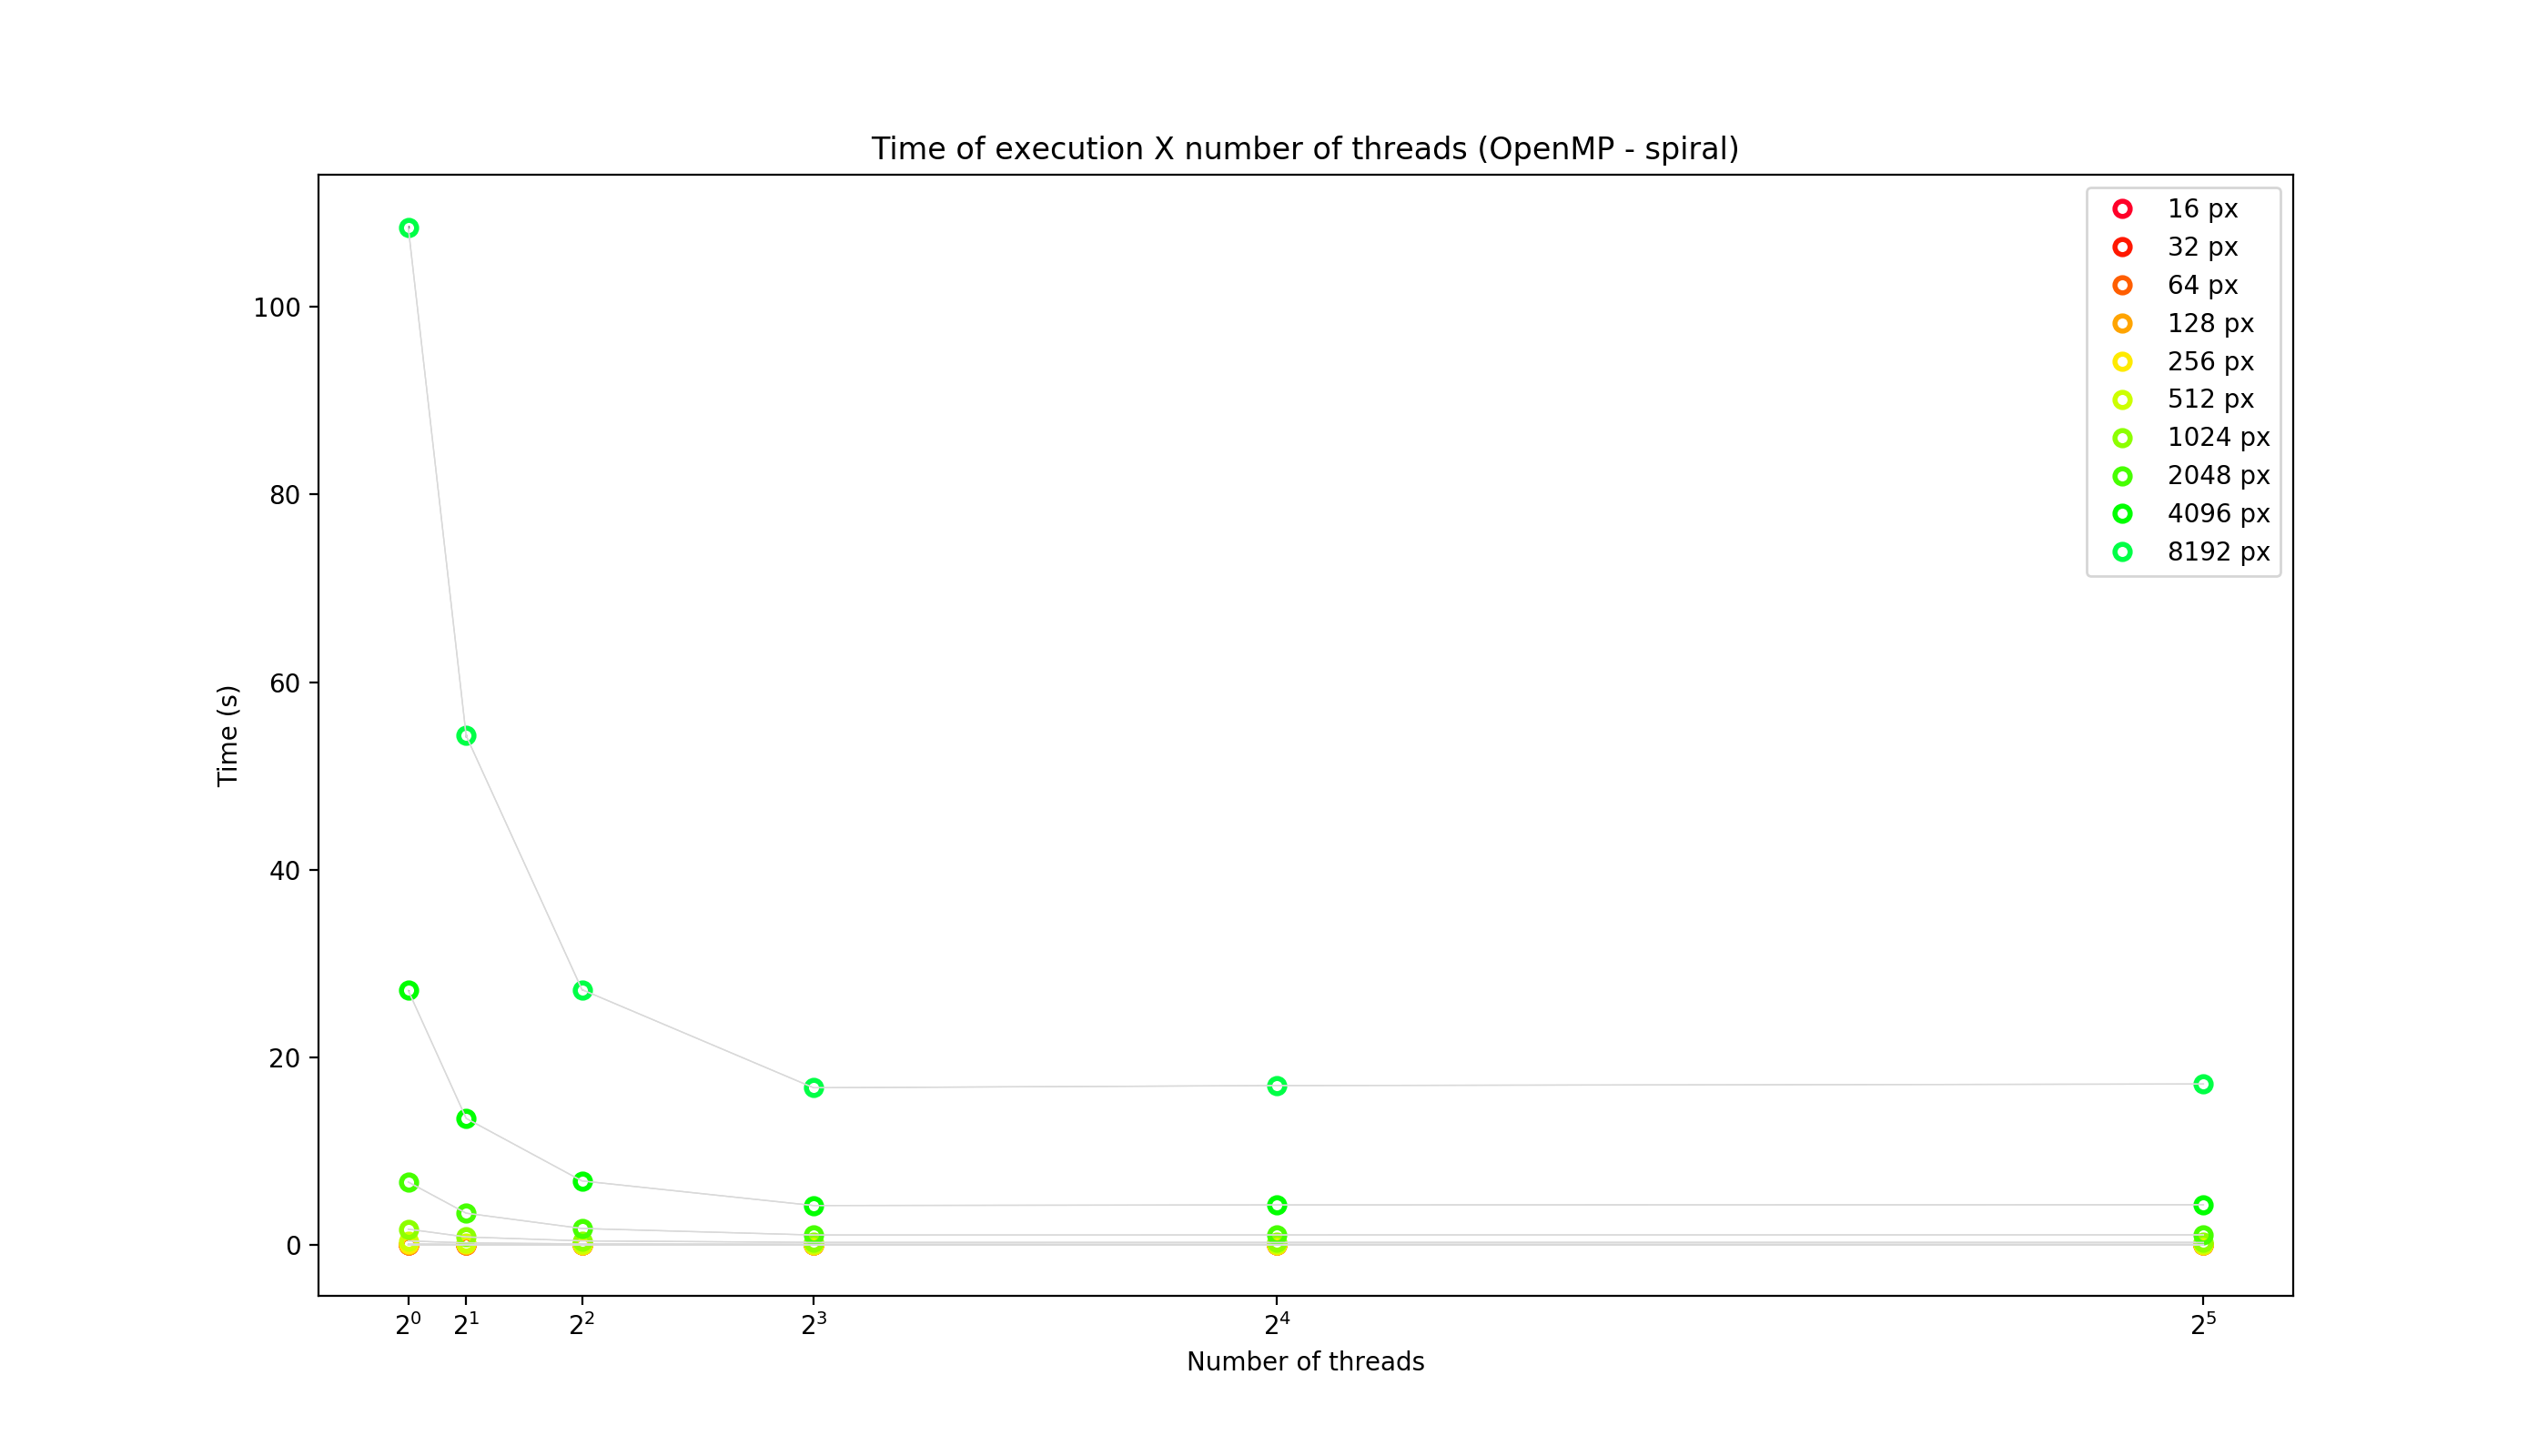
\includegraphics[scale=.50]{for_duplo_plot/timeXthread_spiral_OpenMPpng.png}}
\end{figure}

Nota-se que nessas regiões apesar do comportamento do tempo X numero de threads manter-se o mesmo, o tempo de execução aumenta, pois nessas regiões há mais cálculos de pontos com mais interações. Podemos comparar todas as regiões:

\begin{figure}[H]
    \makebox[\textwidth][c]{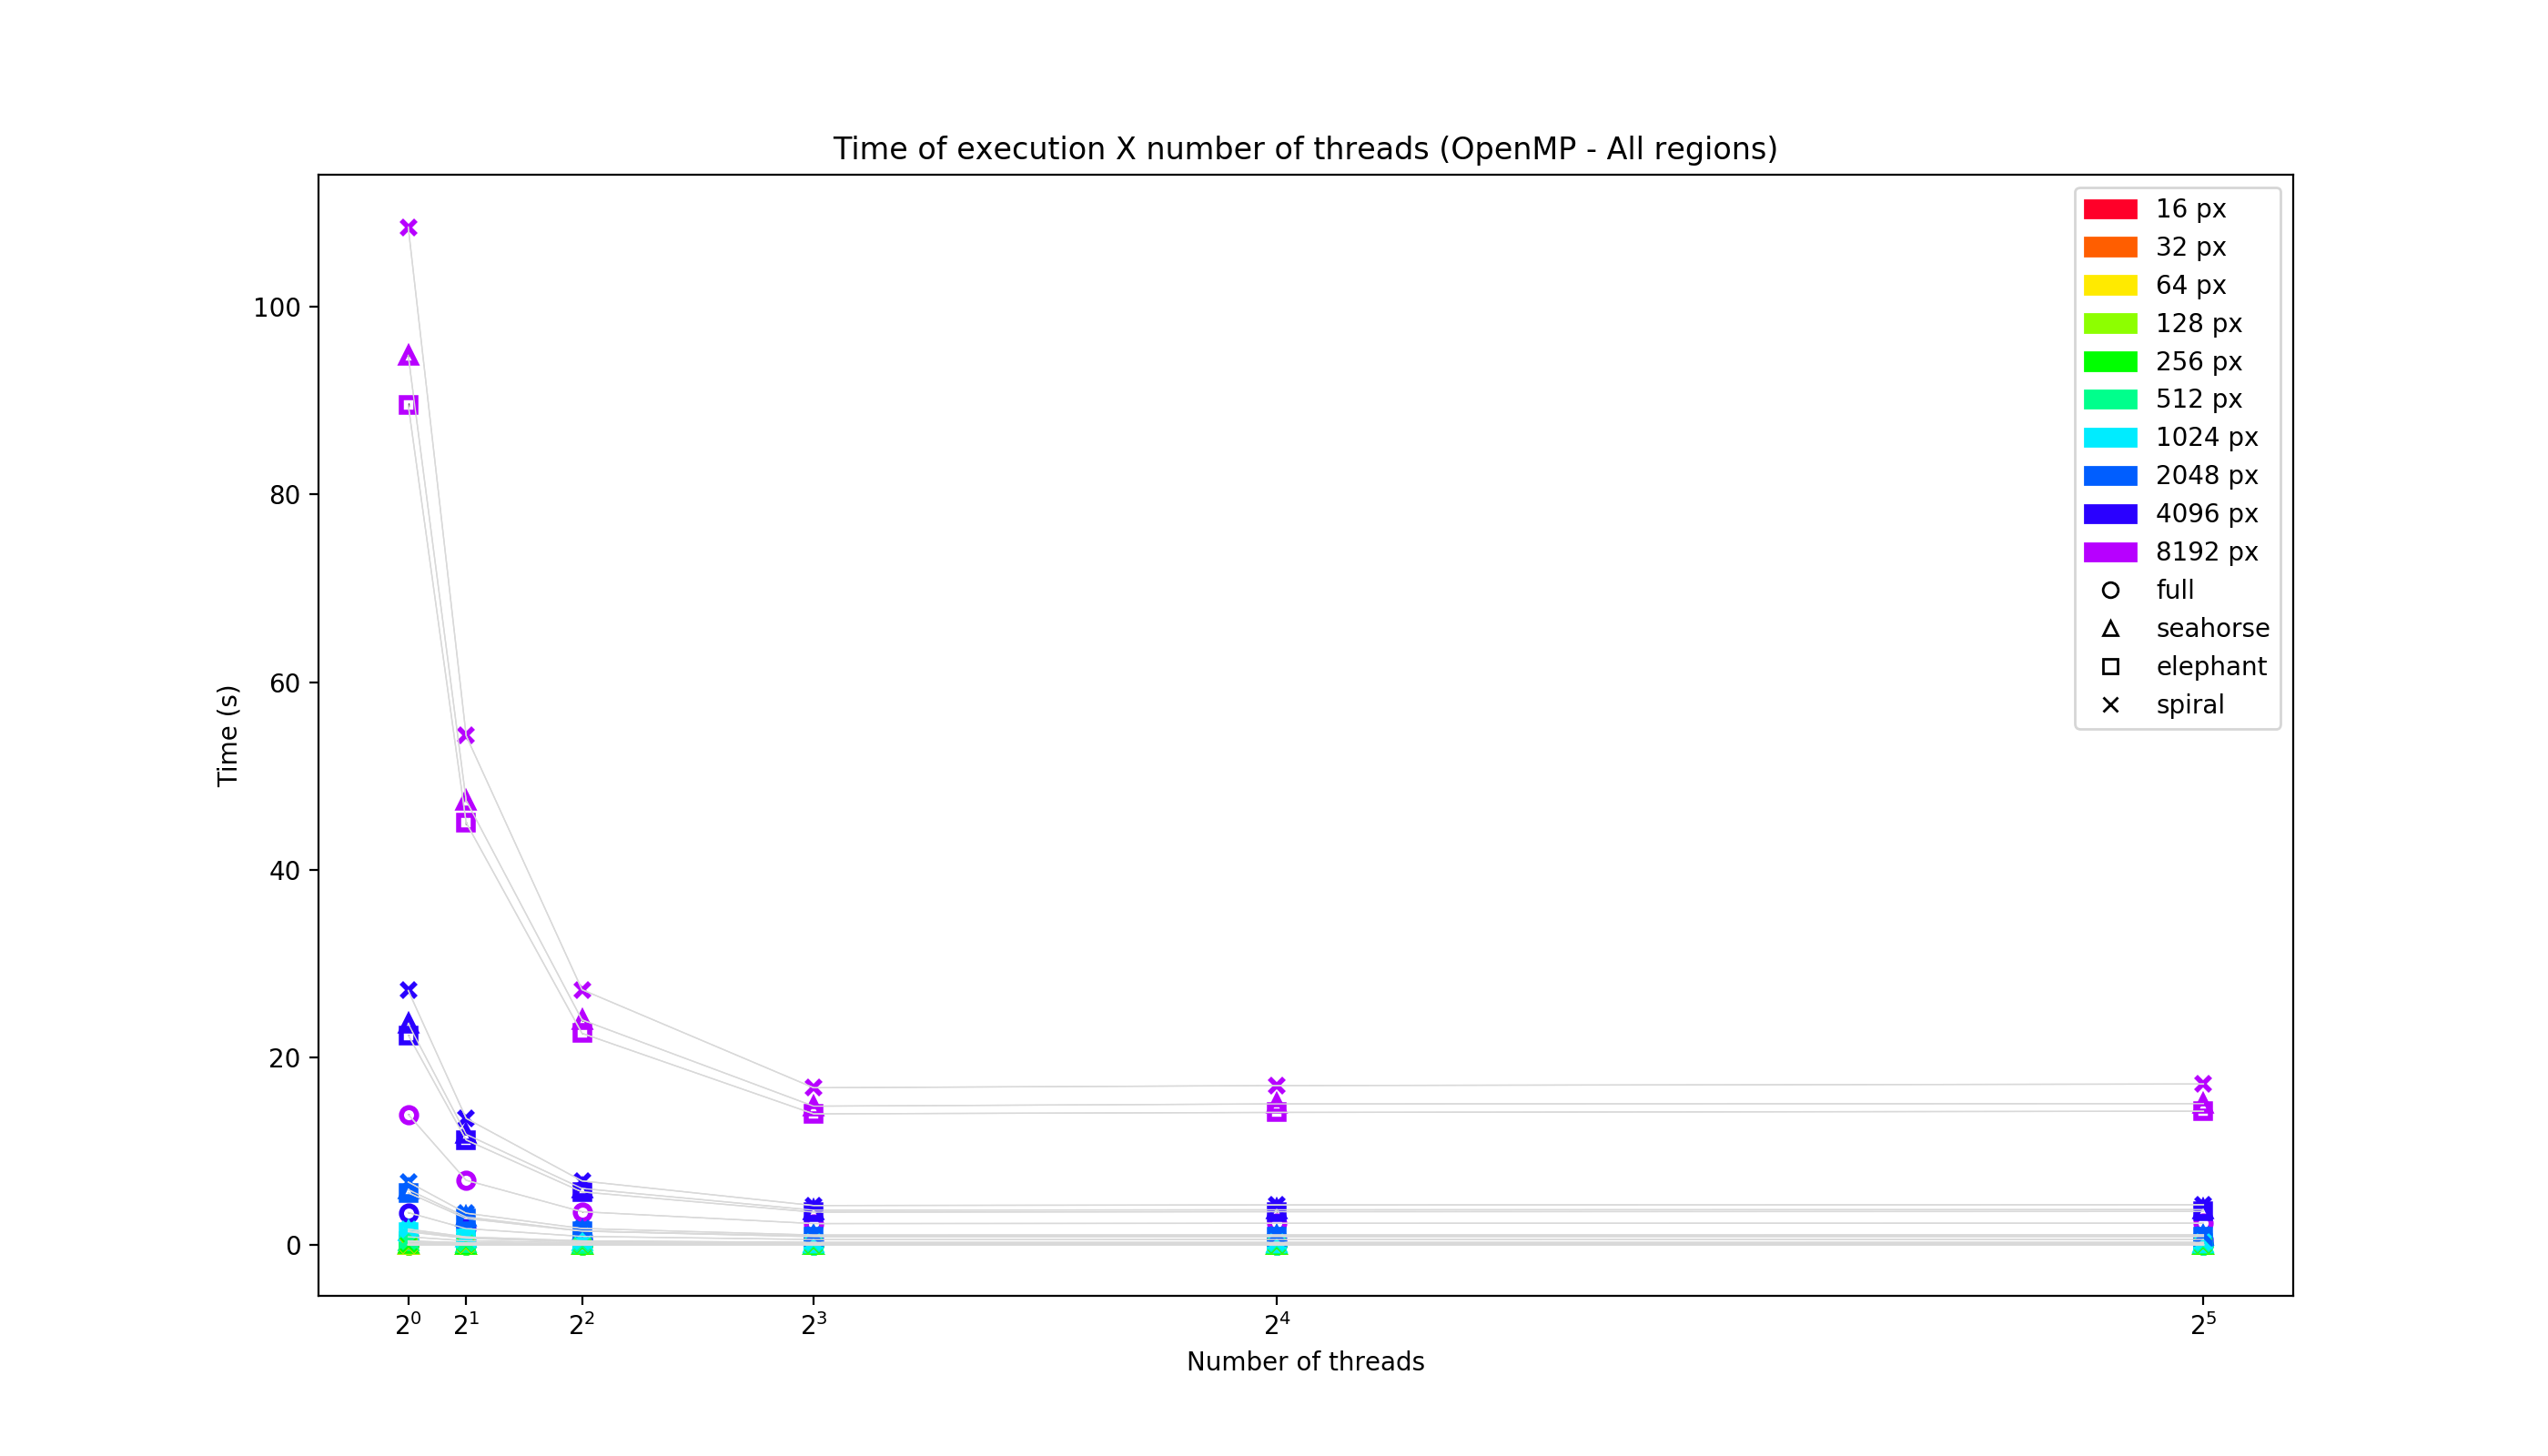
\includegraphics[scale=.50]{for_duplo_plot/all_timeXthread_OpenMPpng.png}}
\end{figure}

Vemos que as regiões Spiral, Seahorse e Elephant tem tempo de execução bastante maior que a região Full.

Em todos esses gráficos também vemos que quanto maior o tamanho da entrada, mais tempo o programa leva para ser executado. Porém também queremos saber qual é a relação entre tamanho de entrada e o tempo:

\begin{figure}[H]
    \makebox[\textwidth][c]{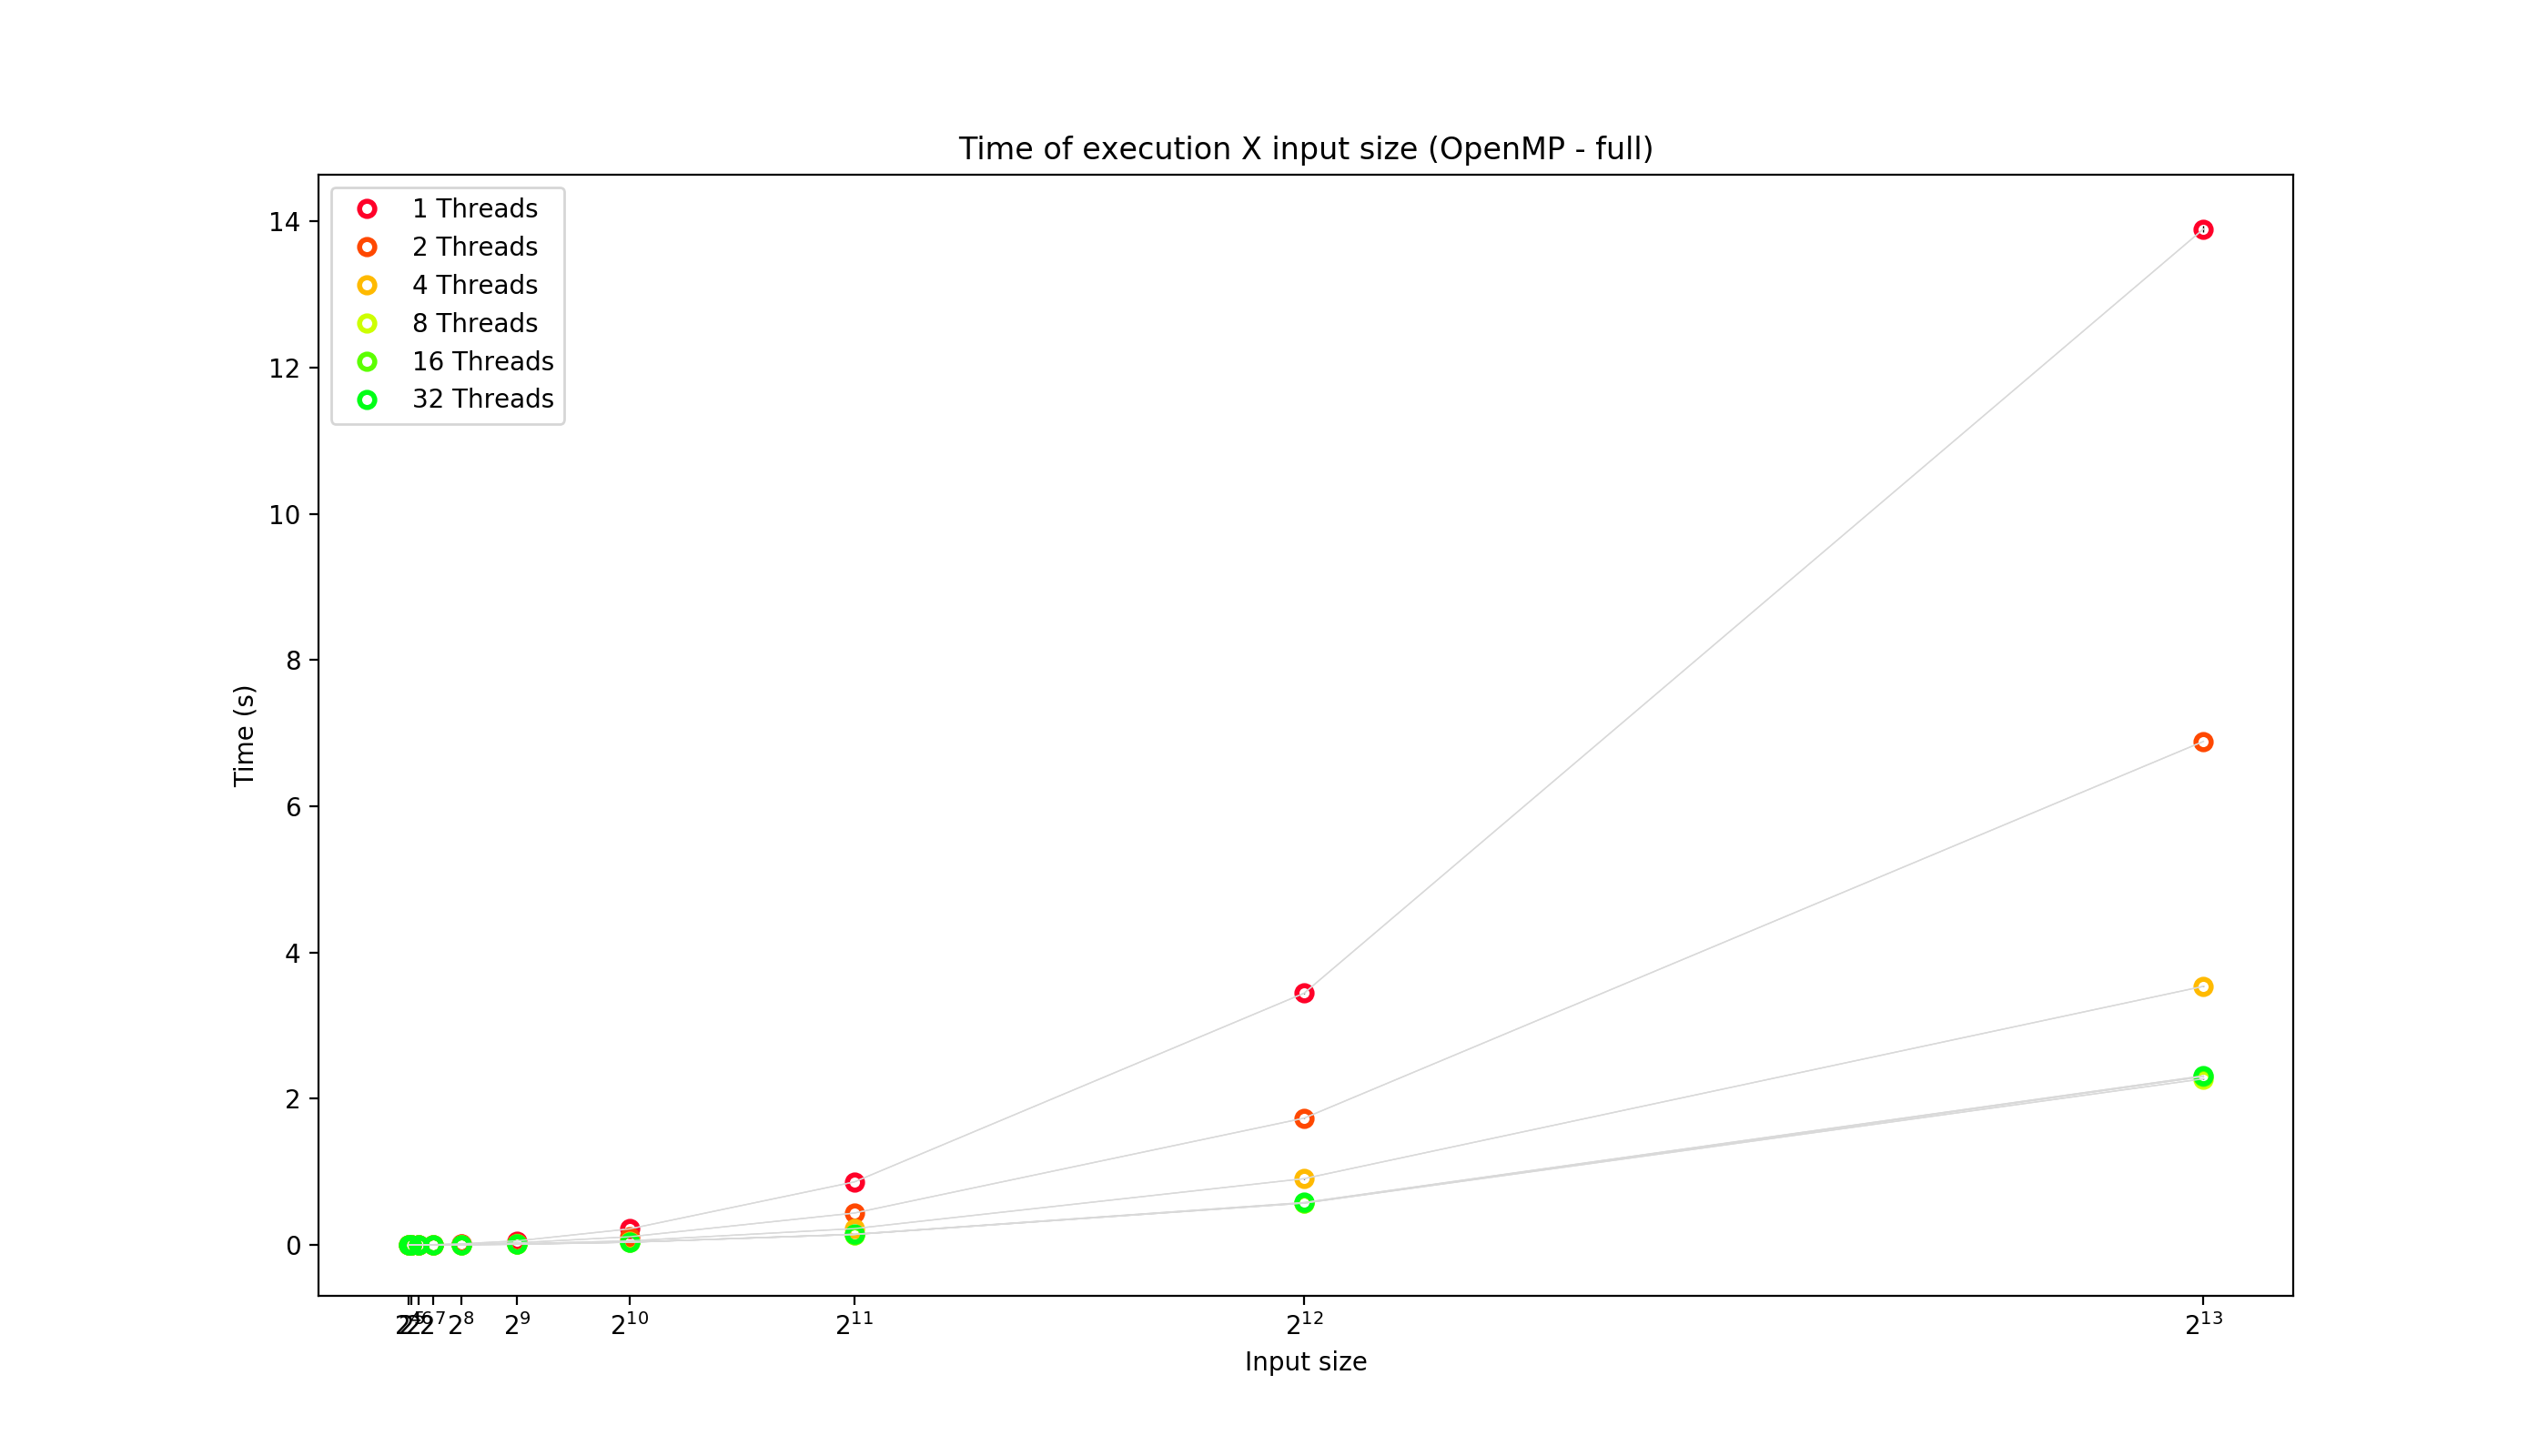
\includegraphics[scale=.50]{for_duplo_plot/timeXsize_full_OpenMPpng.png}}
\end{figure}

Vemos que há um aumento exponencial do tempo pelo tamanho da imagem. Vale lembrar que consideramos o tamanho de entrada, somente o tamanho do lado da imagem, portanto o comportamento exponencial se justifica por o número de pixels (chamadas para a função \code{compute\_manderbolt()}) ser o tamanho do lado da imagem elevado ao quadrado.

Nas demais regiões o comportamento é semelhante:

\begin{figure}[H]
    \makebox[\textwidth][c]{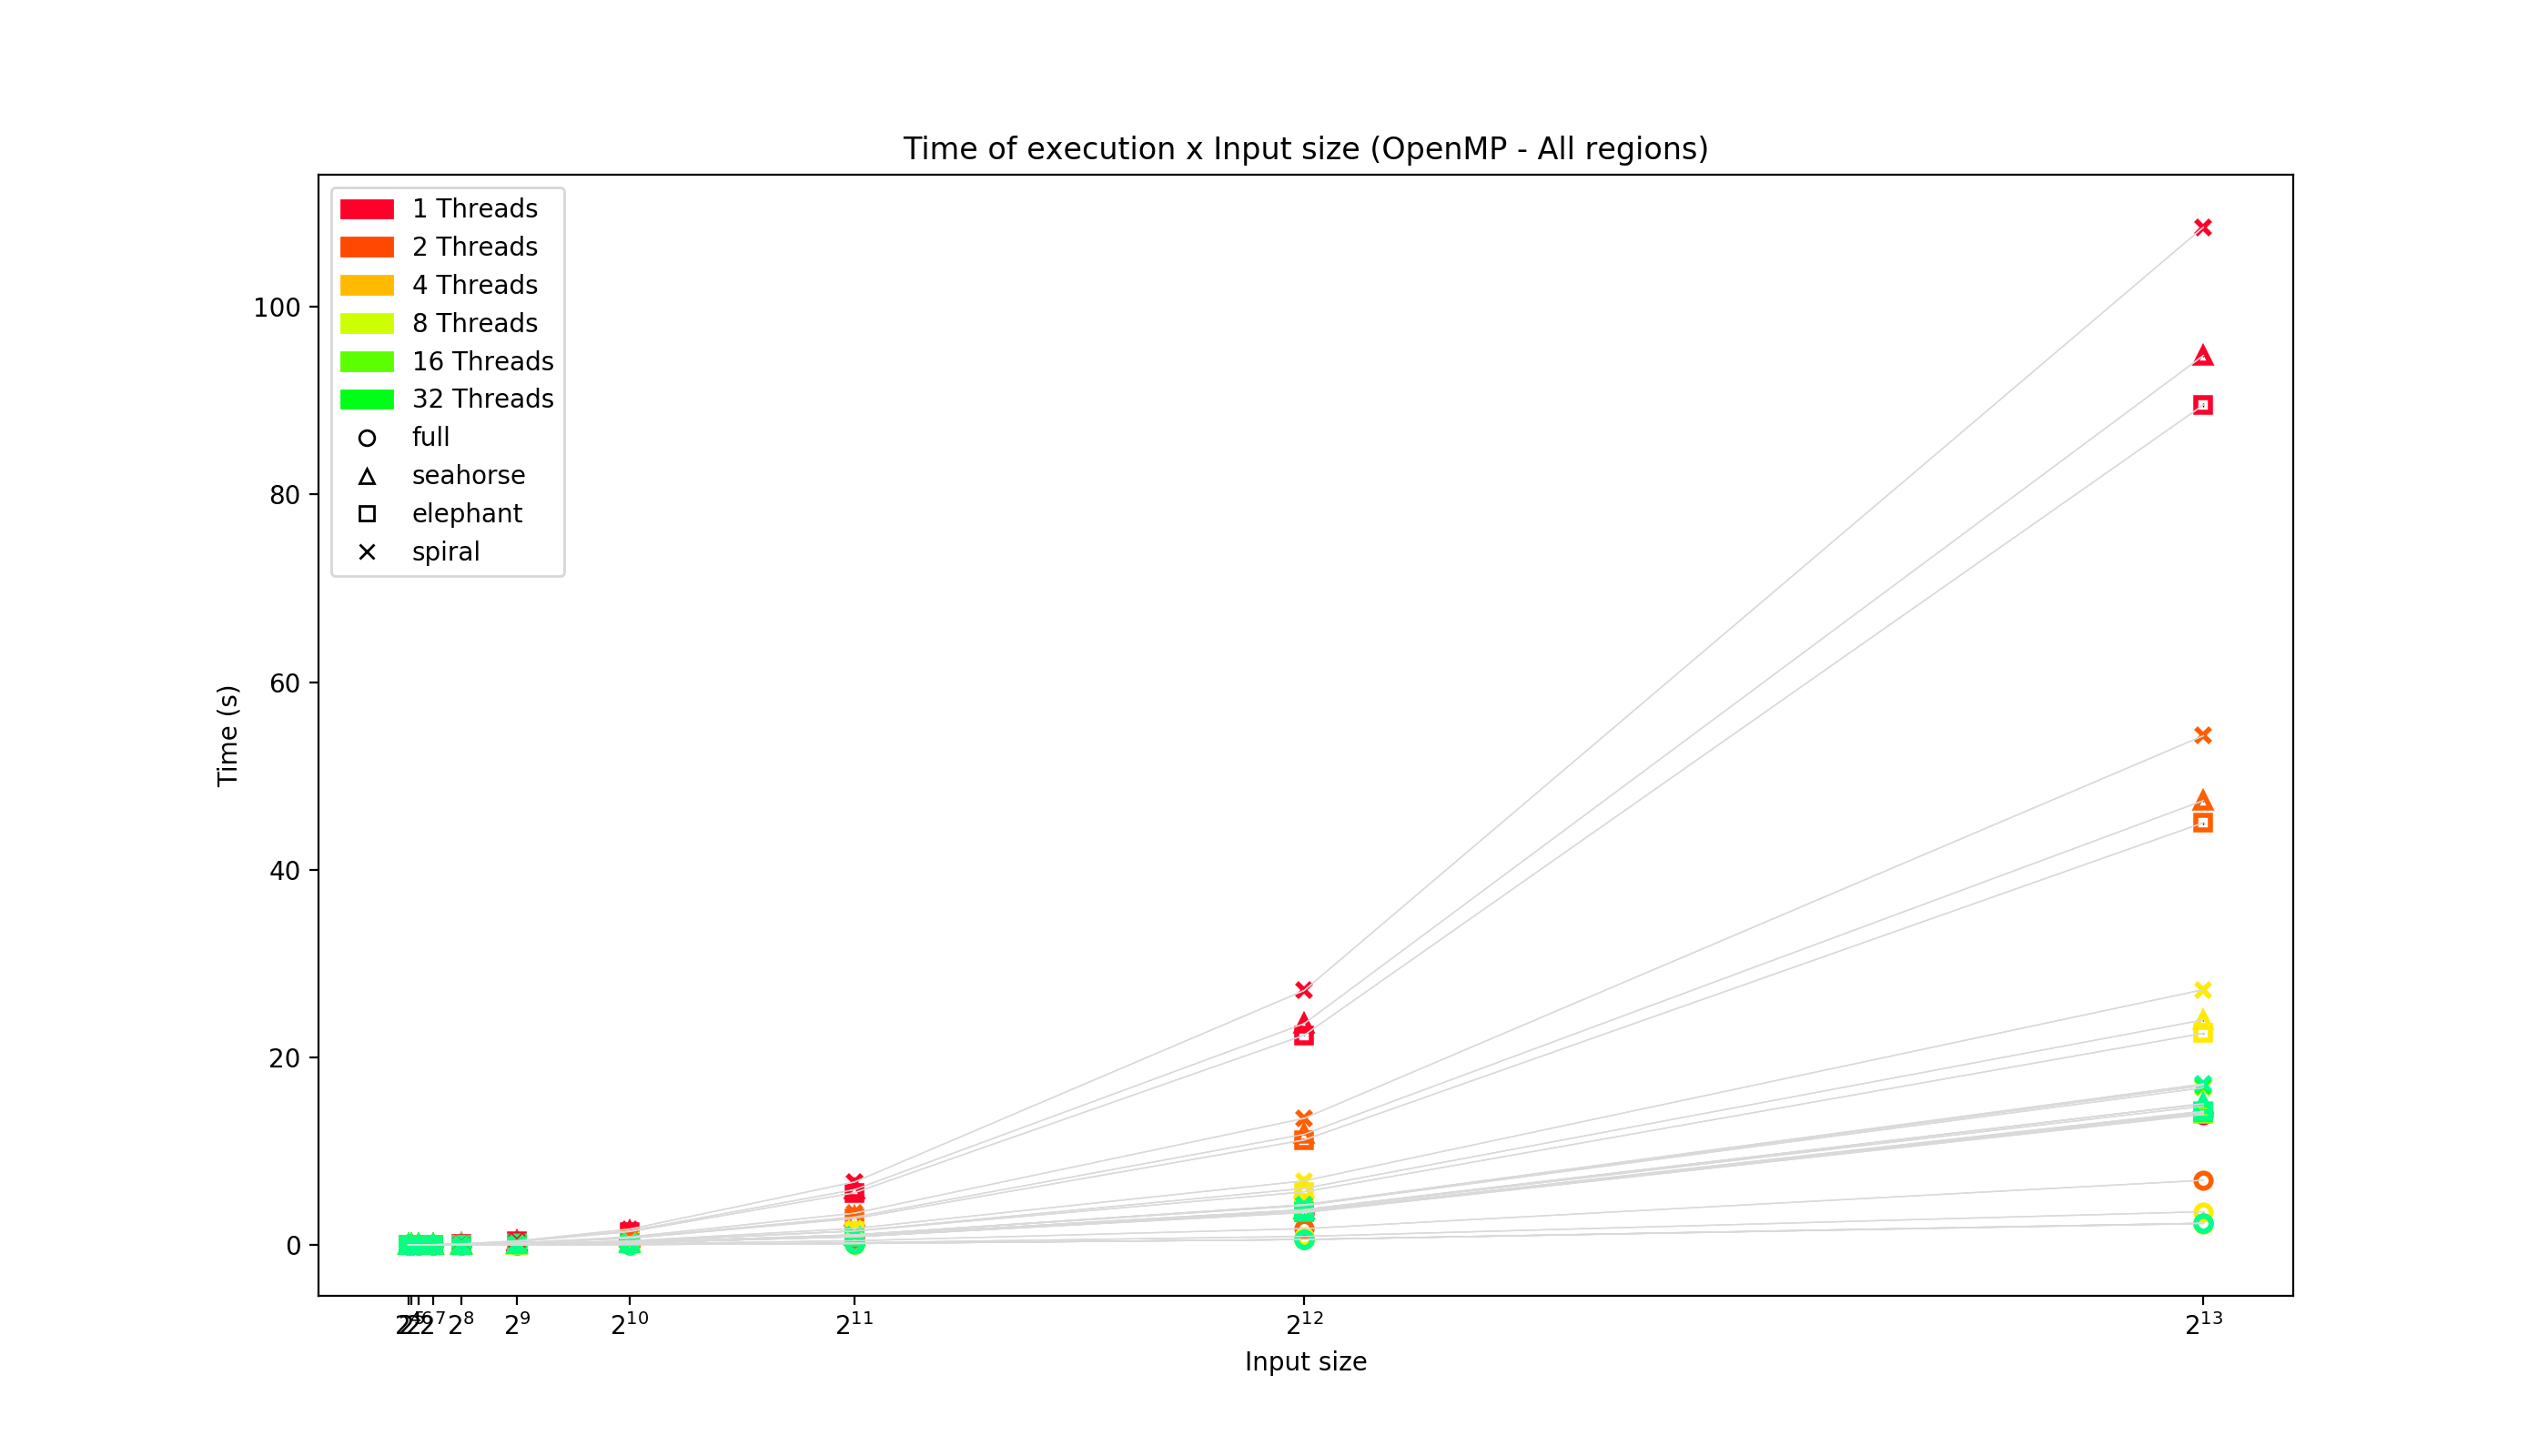
\includegraphics[scale=.50]{for_duplo_plot/all_timeXsize_OpenMPpng.png}}
\end{figure}


Outra API usada na paralelização é o OpenMP. Pela natureza do cálculo do conjunto Mandelbrot, como cada iteração possui tempo de execução diferente para cada pixel, utilizamos \textit{dynamic scheduling}, sendo ela que oferece melhor distribuição de trabalho.

\begin{figure}[H]
    \centering
    \begin{tabular}{c c}
        \subfigure[] {\scalebox{.40}{
            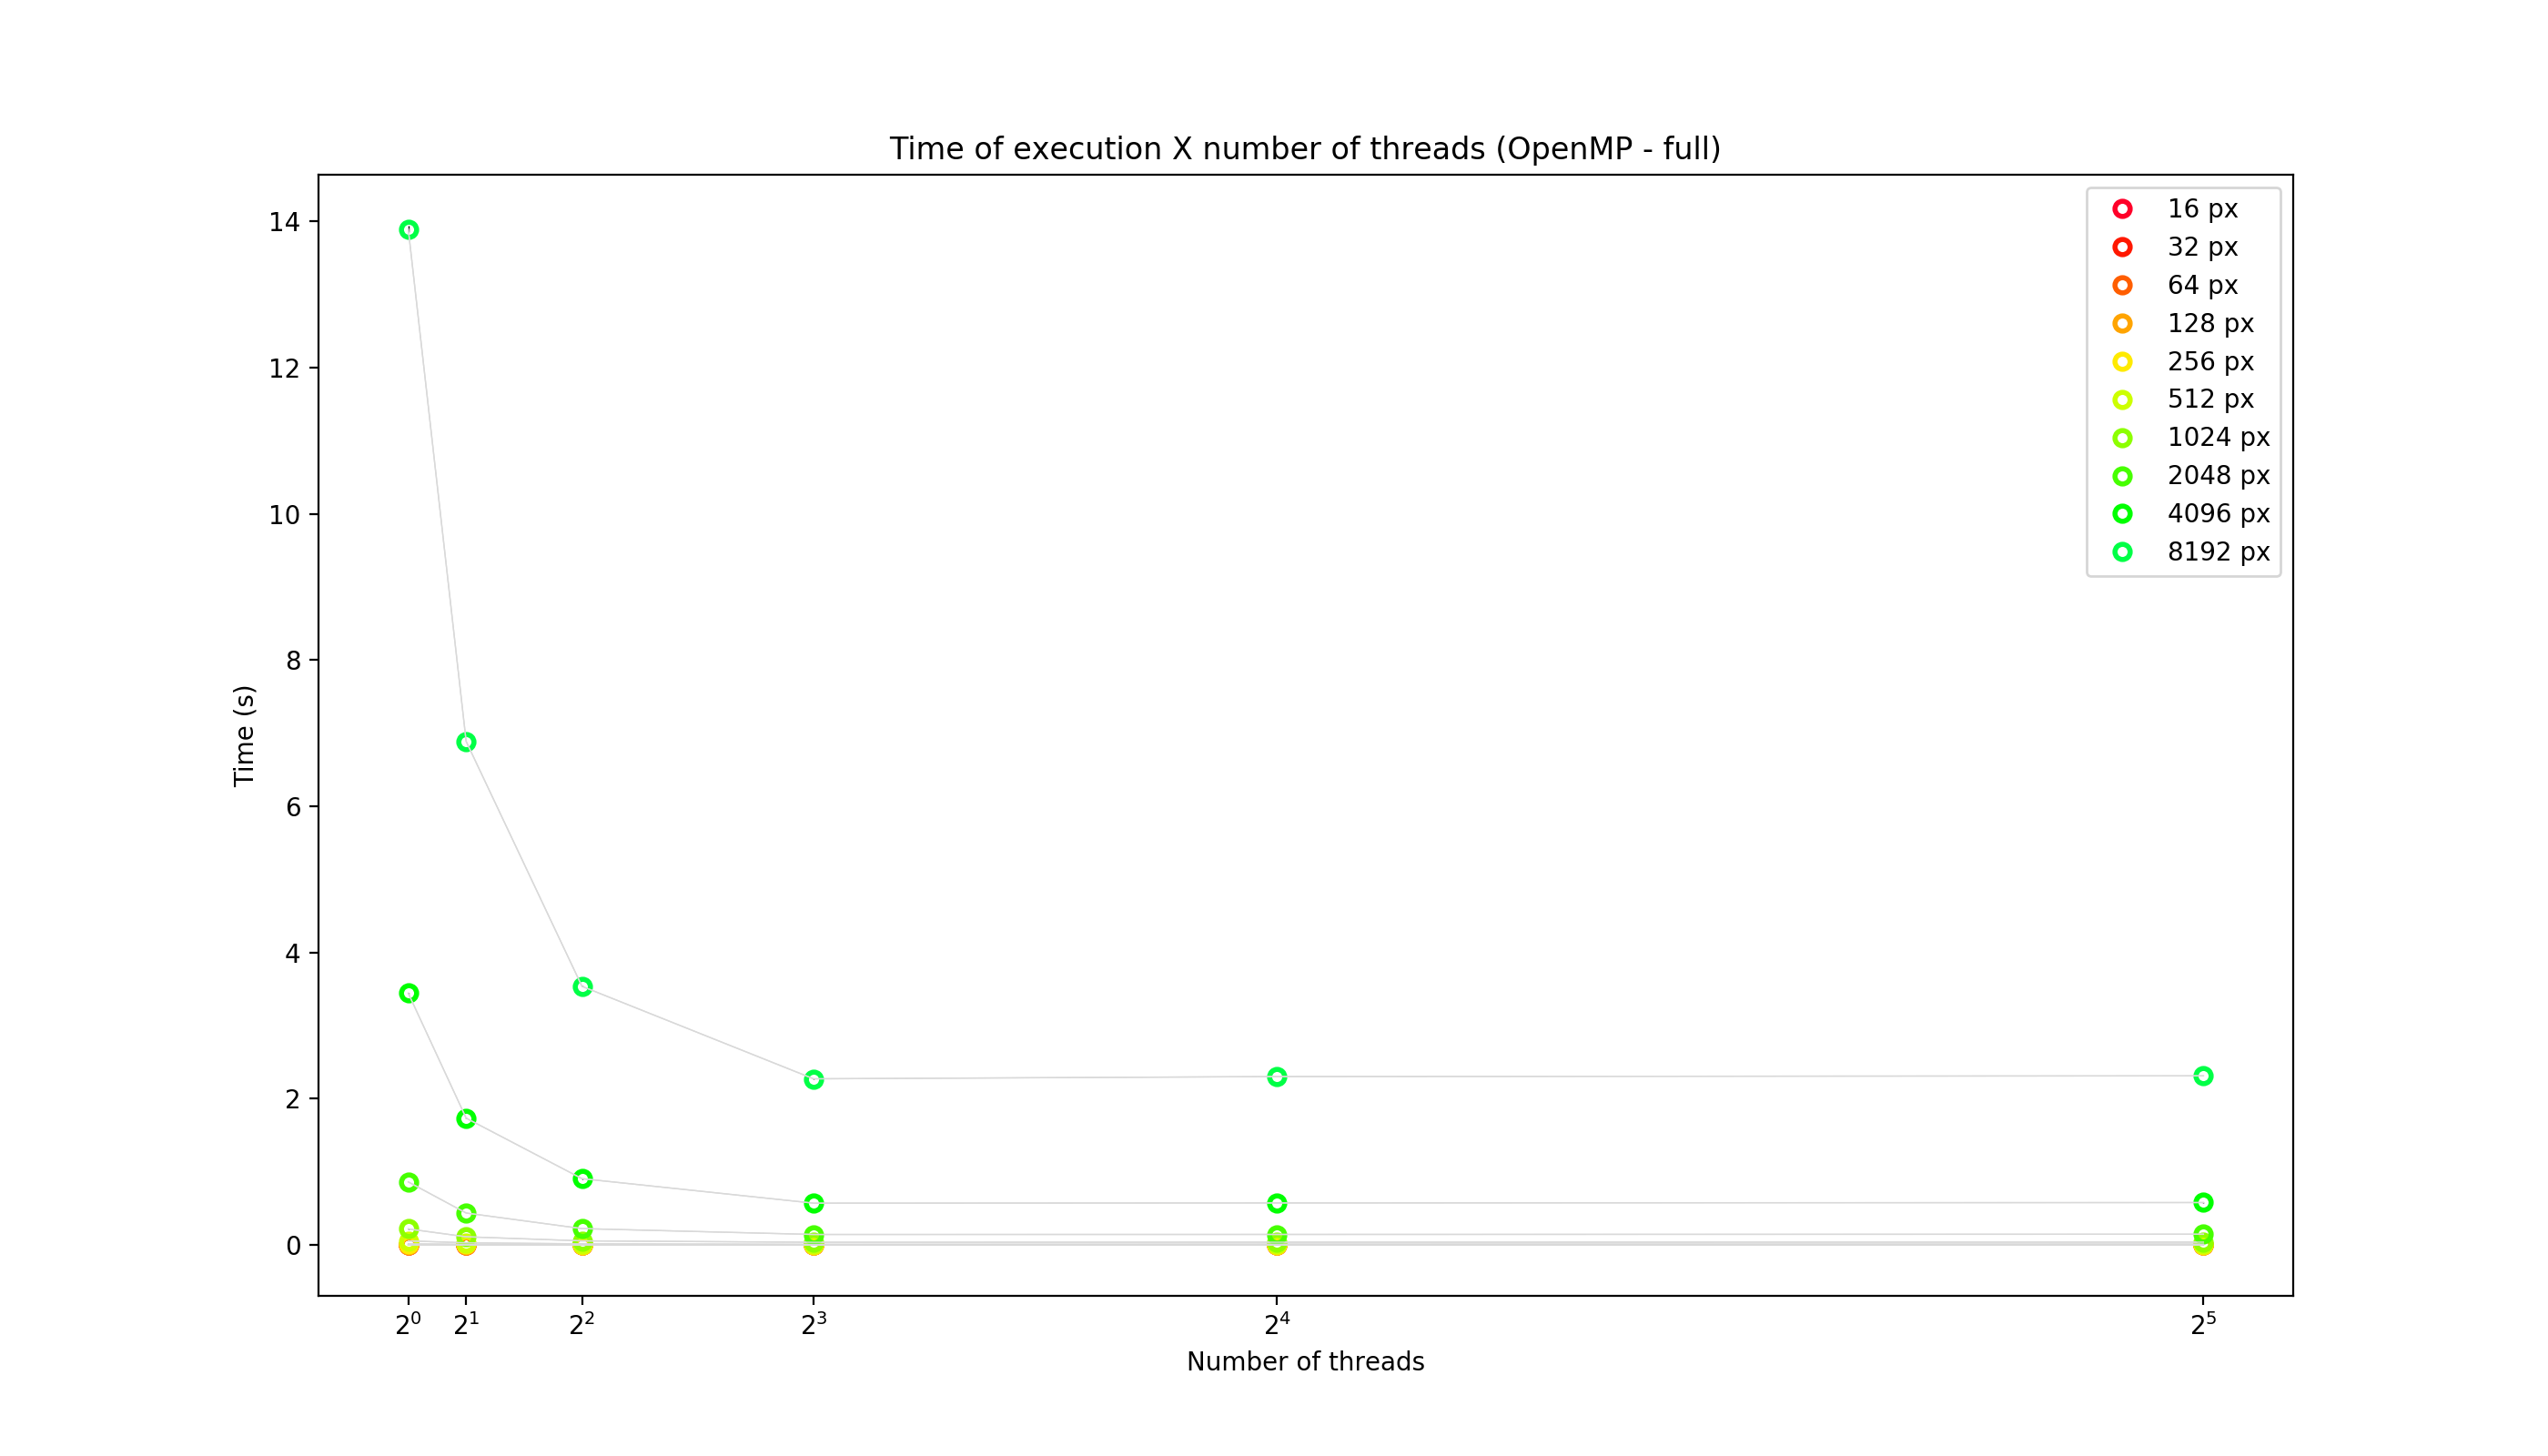
\includegraphics{for_duplo_plot/timeXthread_full_OpenMPpng.png}}
            \label {fig:omp_all:A}
        }
        \\
        \subfigure[] {\scalebox{.40}{
        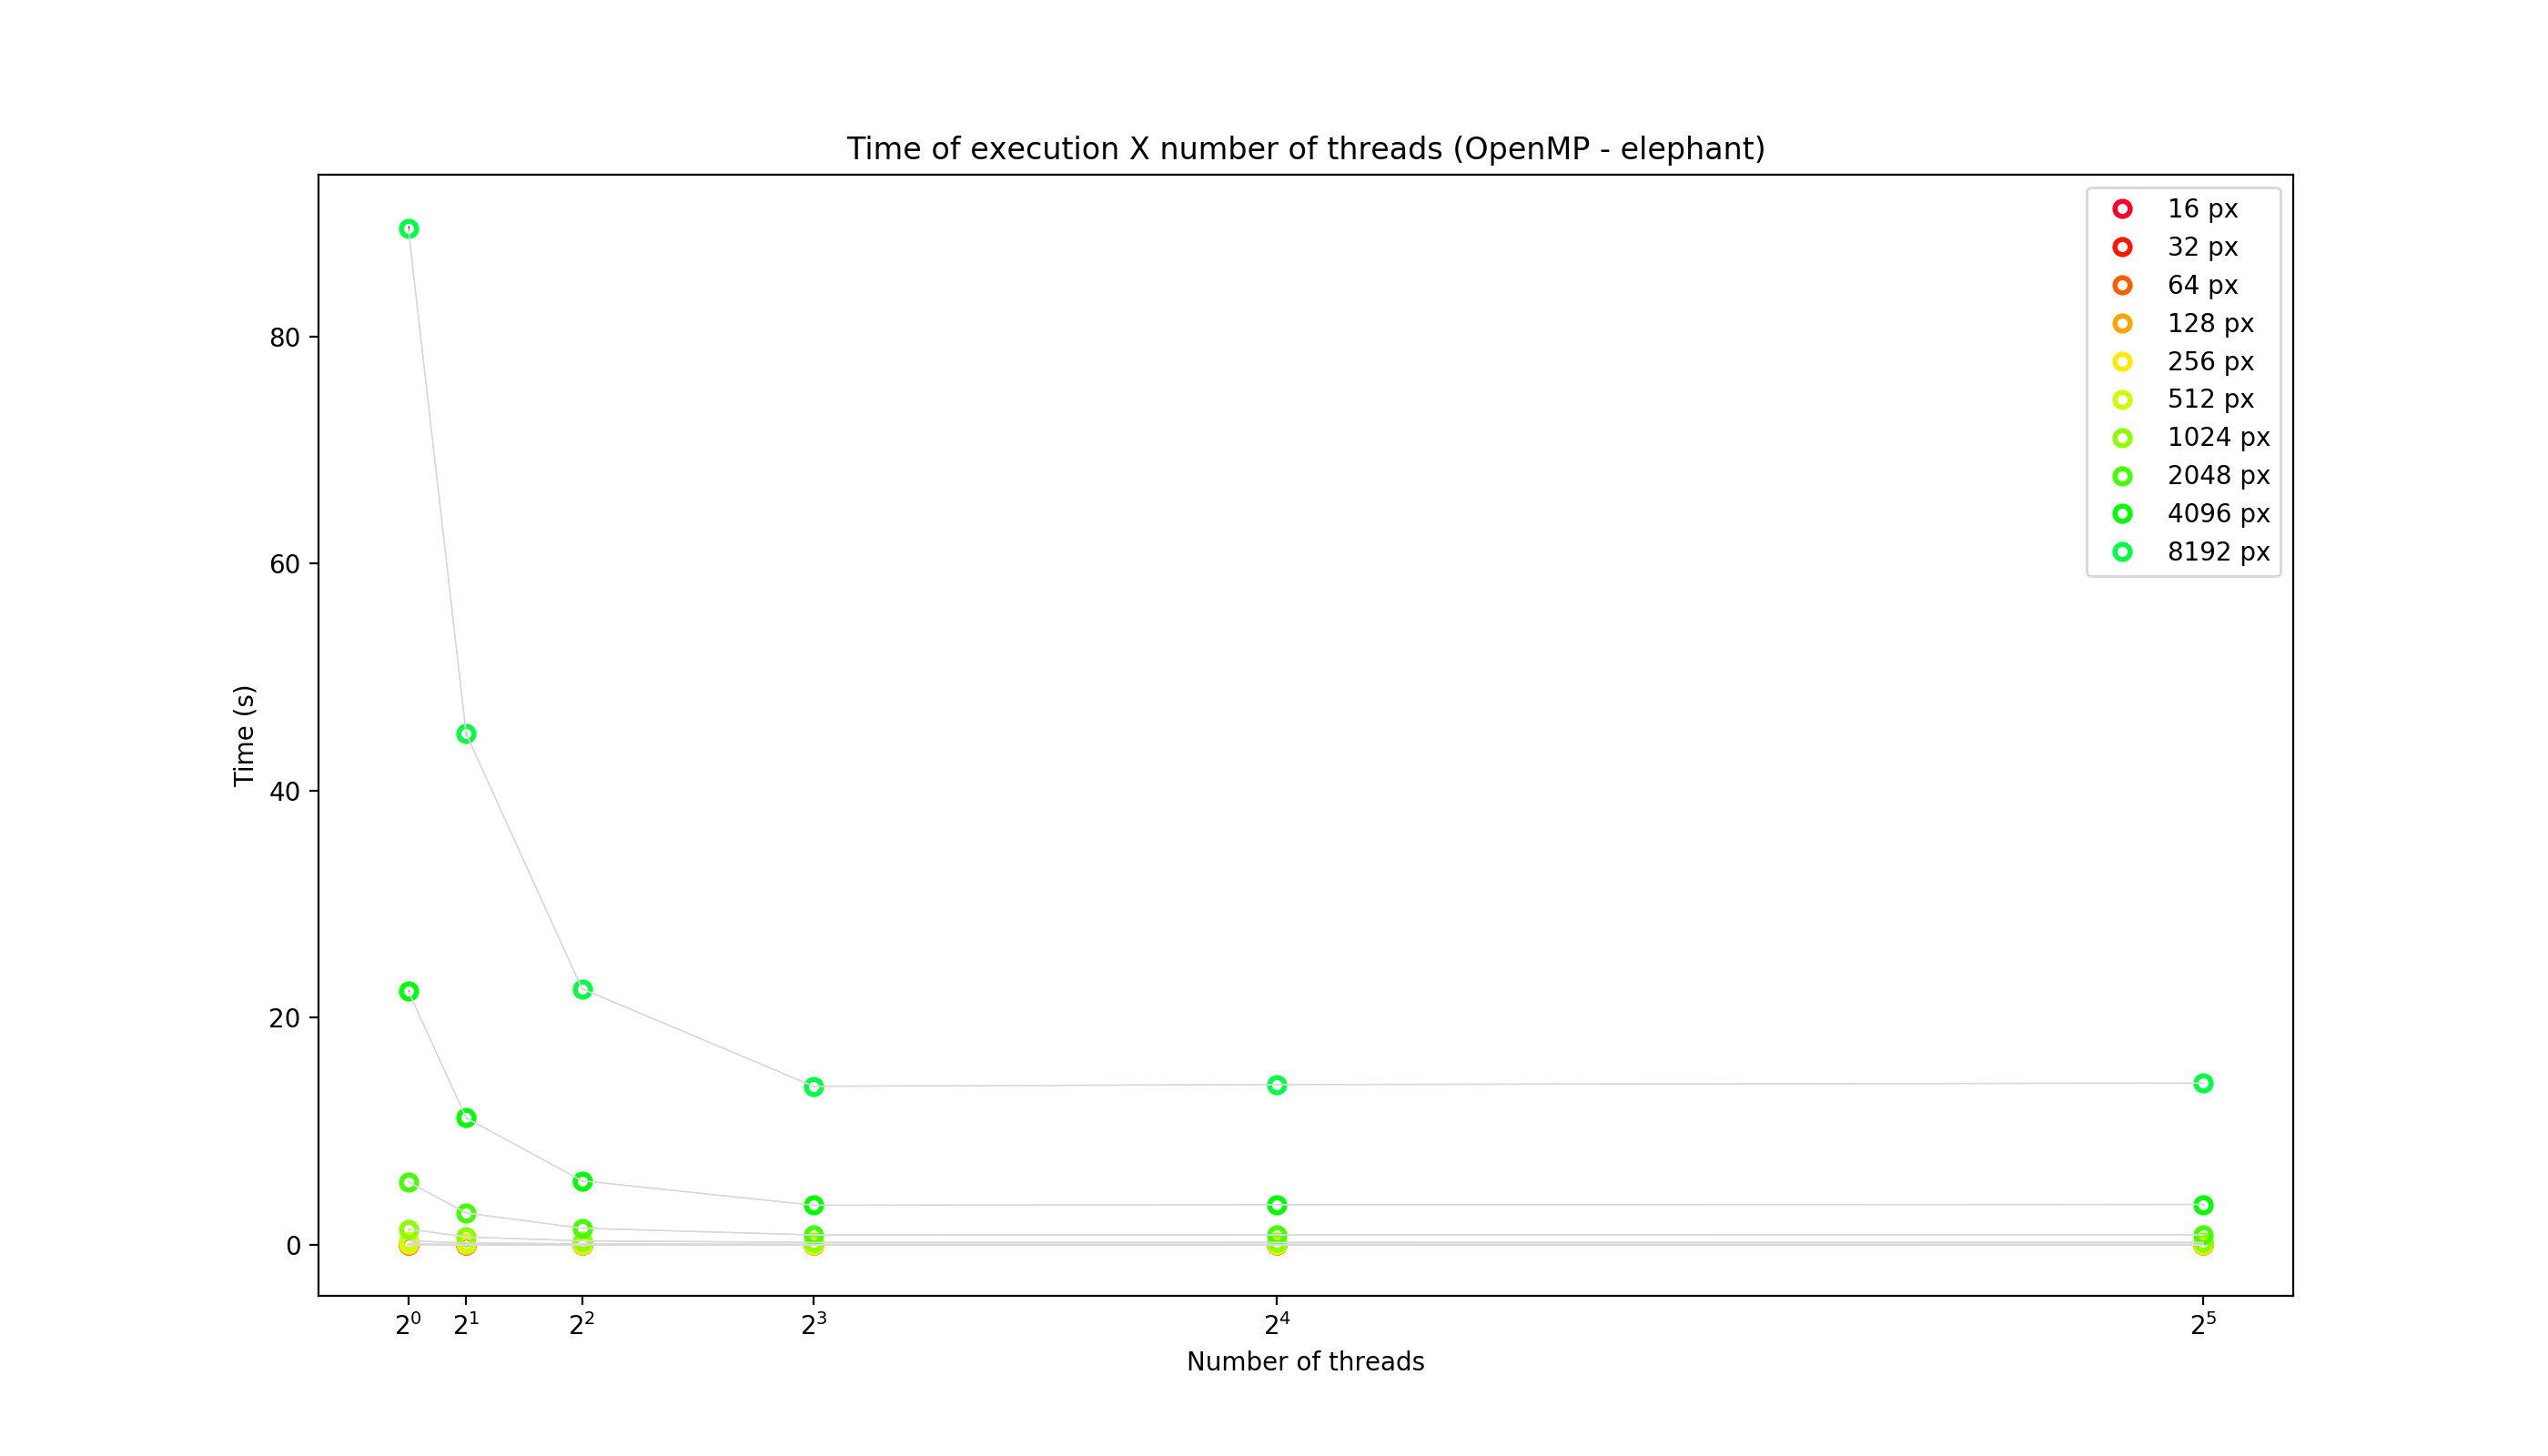
\includegraphics{for_duplo_plot/timeXthread_elephant_OpenMPpng.png}}
            \label {fig:omp_all:B}
        }
    \end{tabular}
    \caption{(b) representa uma ampliação dos dados de imagens de 2048 
    pixels da figura (a) .}
    \label{fig:omp_all} 
\end{figure}

Há um aumento de tempo de execução no cálculo do conjunto de regiões 
ampliadas como *spiral*, *elephant* devido ao maior número de cálculos 
envolvidos em uma região ampliada do nosso conjunto.

\begin{figure}[H]
    \centering
    \begin{tabular}{c c}
        \subfigure[] {\scalebox{.20}{
            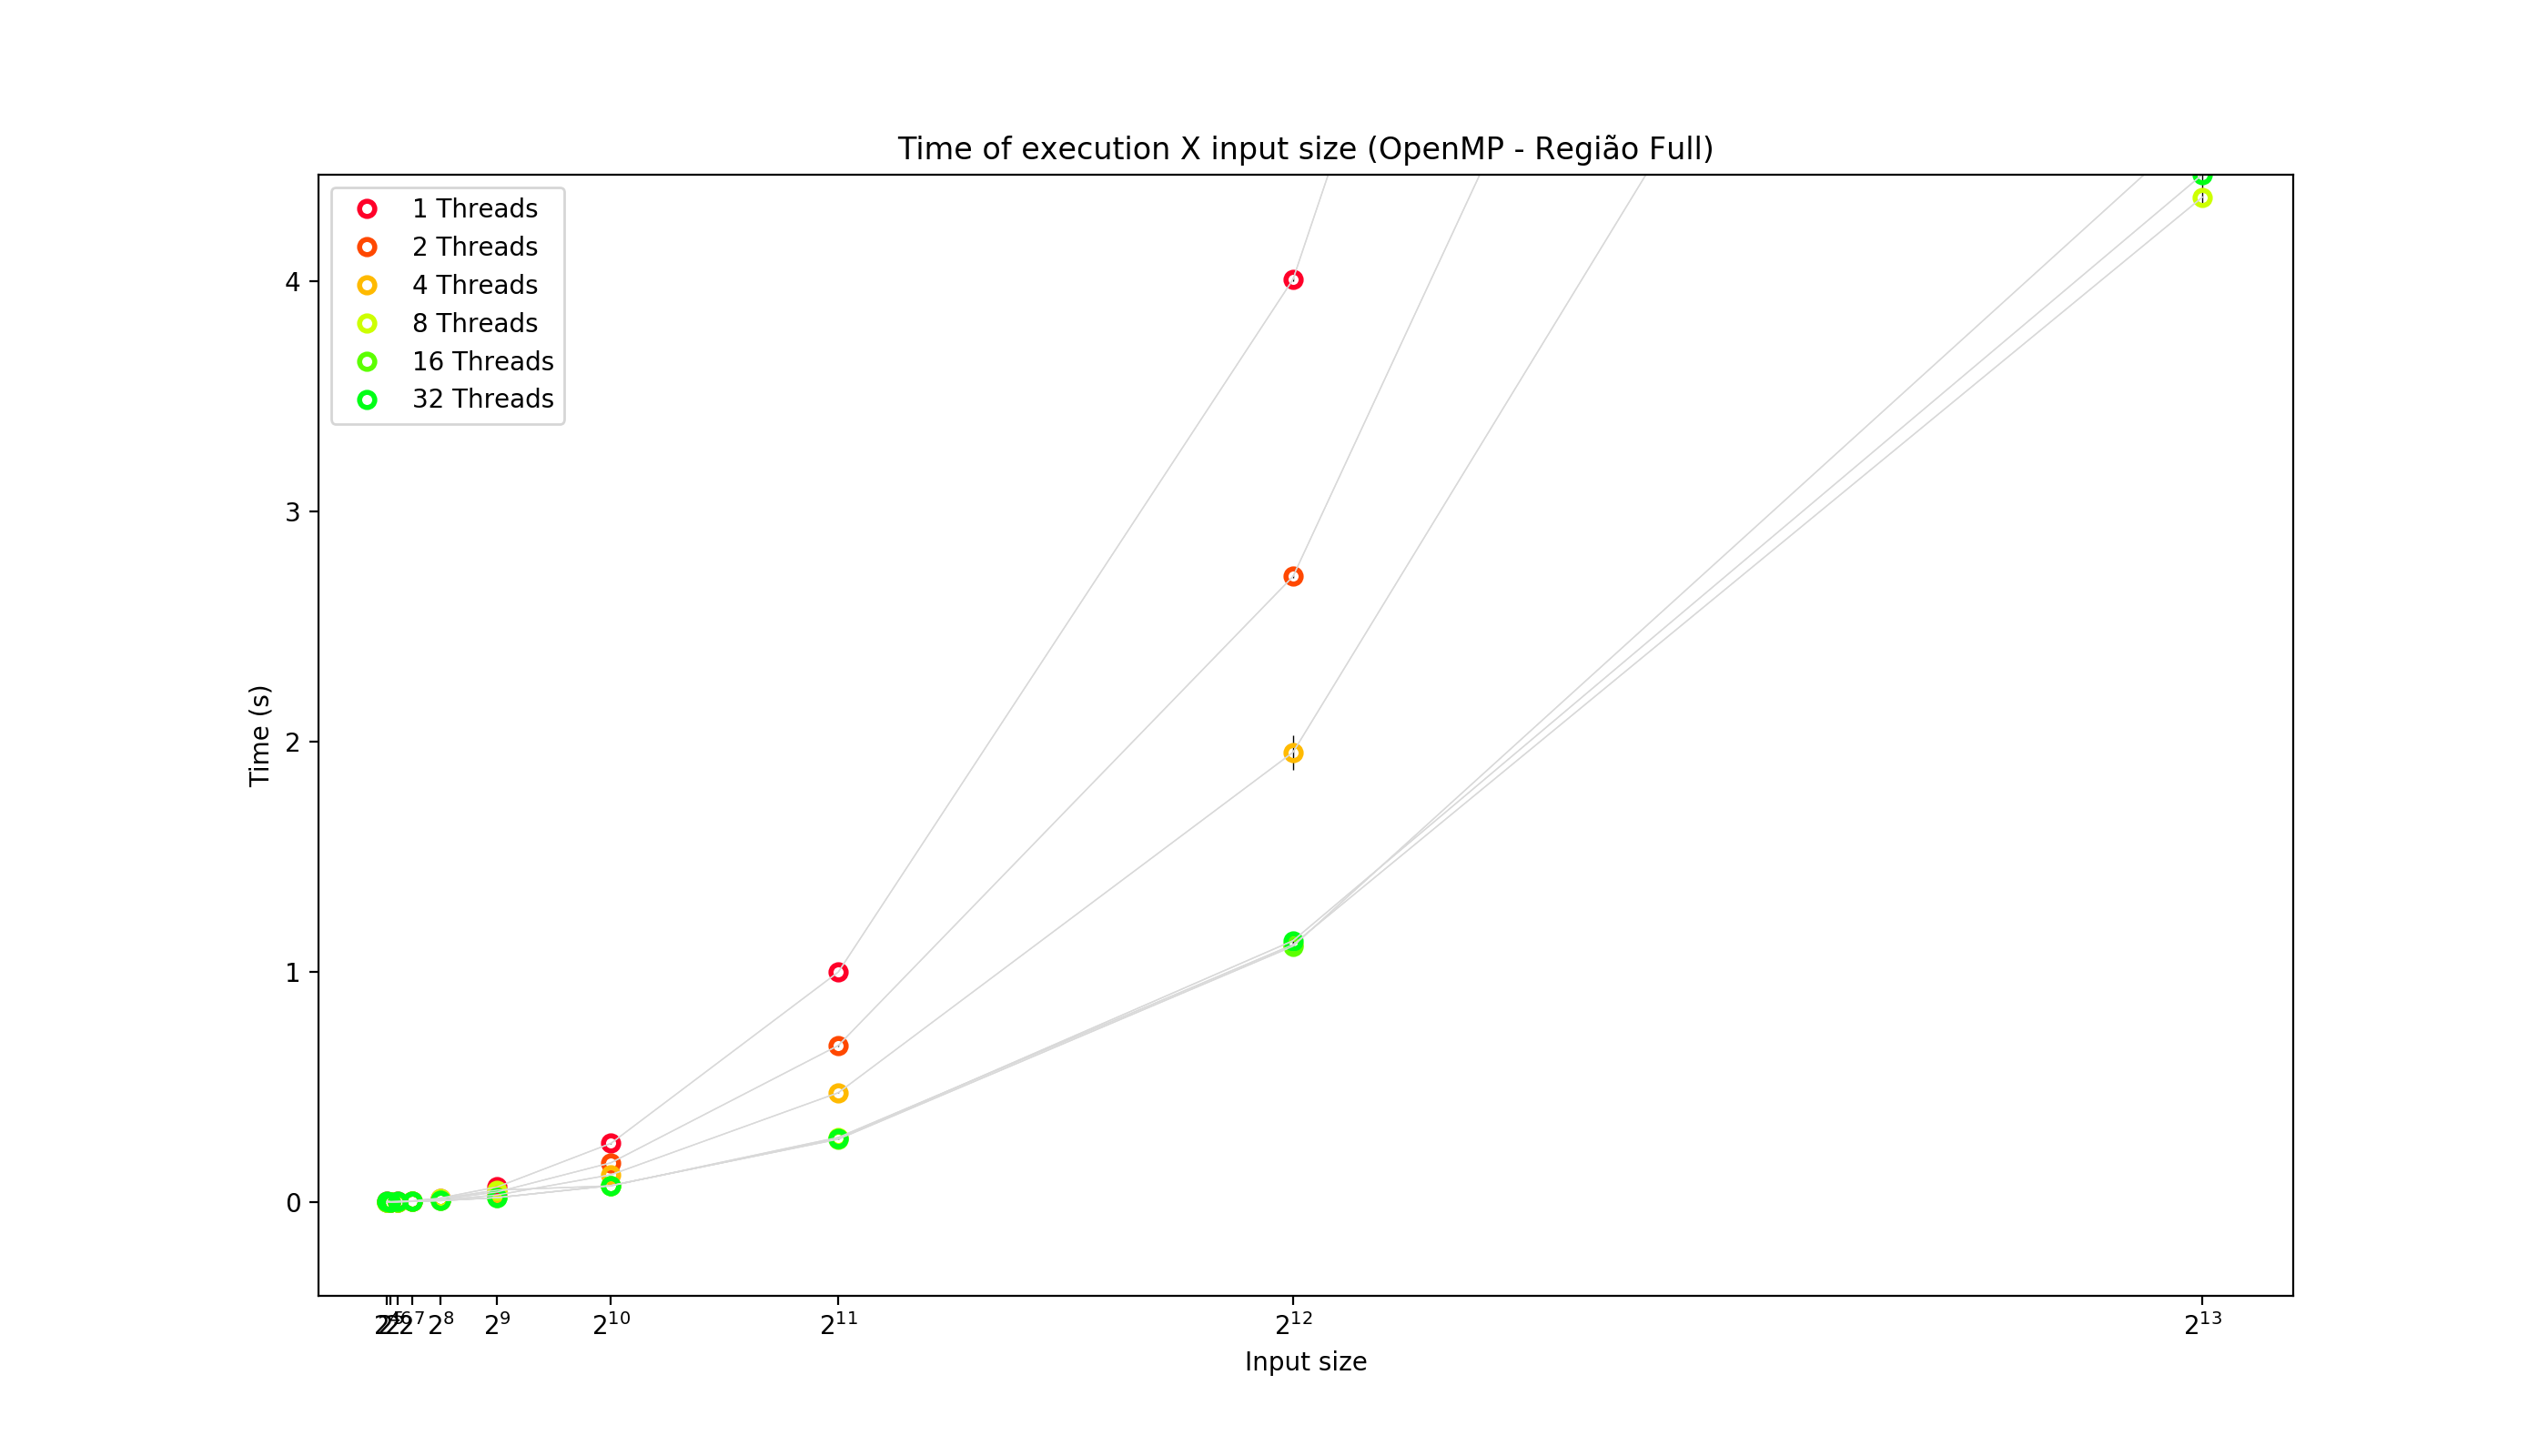
\includegraphics{omp_full/time_input_omp_minor_values.png}}
            \label {fig:omp_full:A}
        }
        &
        \subfigure[] {\scalebox{.20}{
        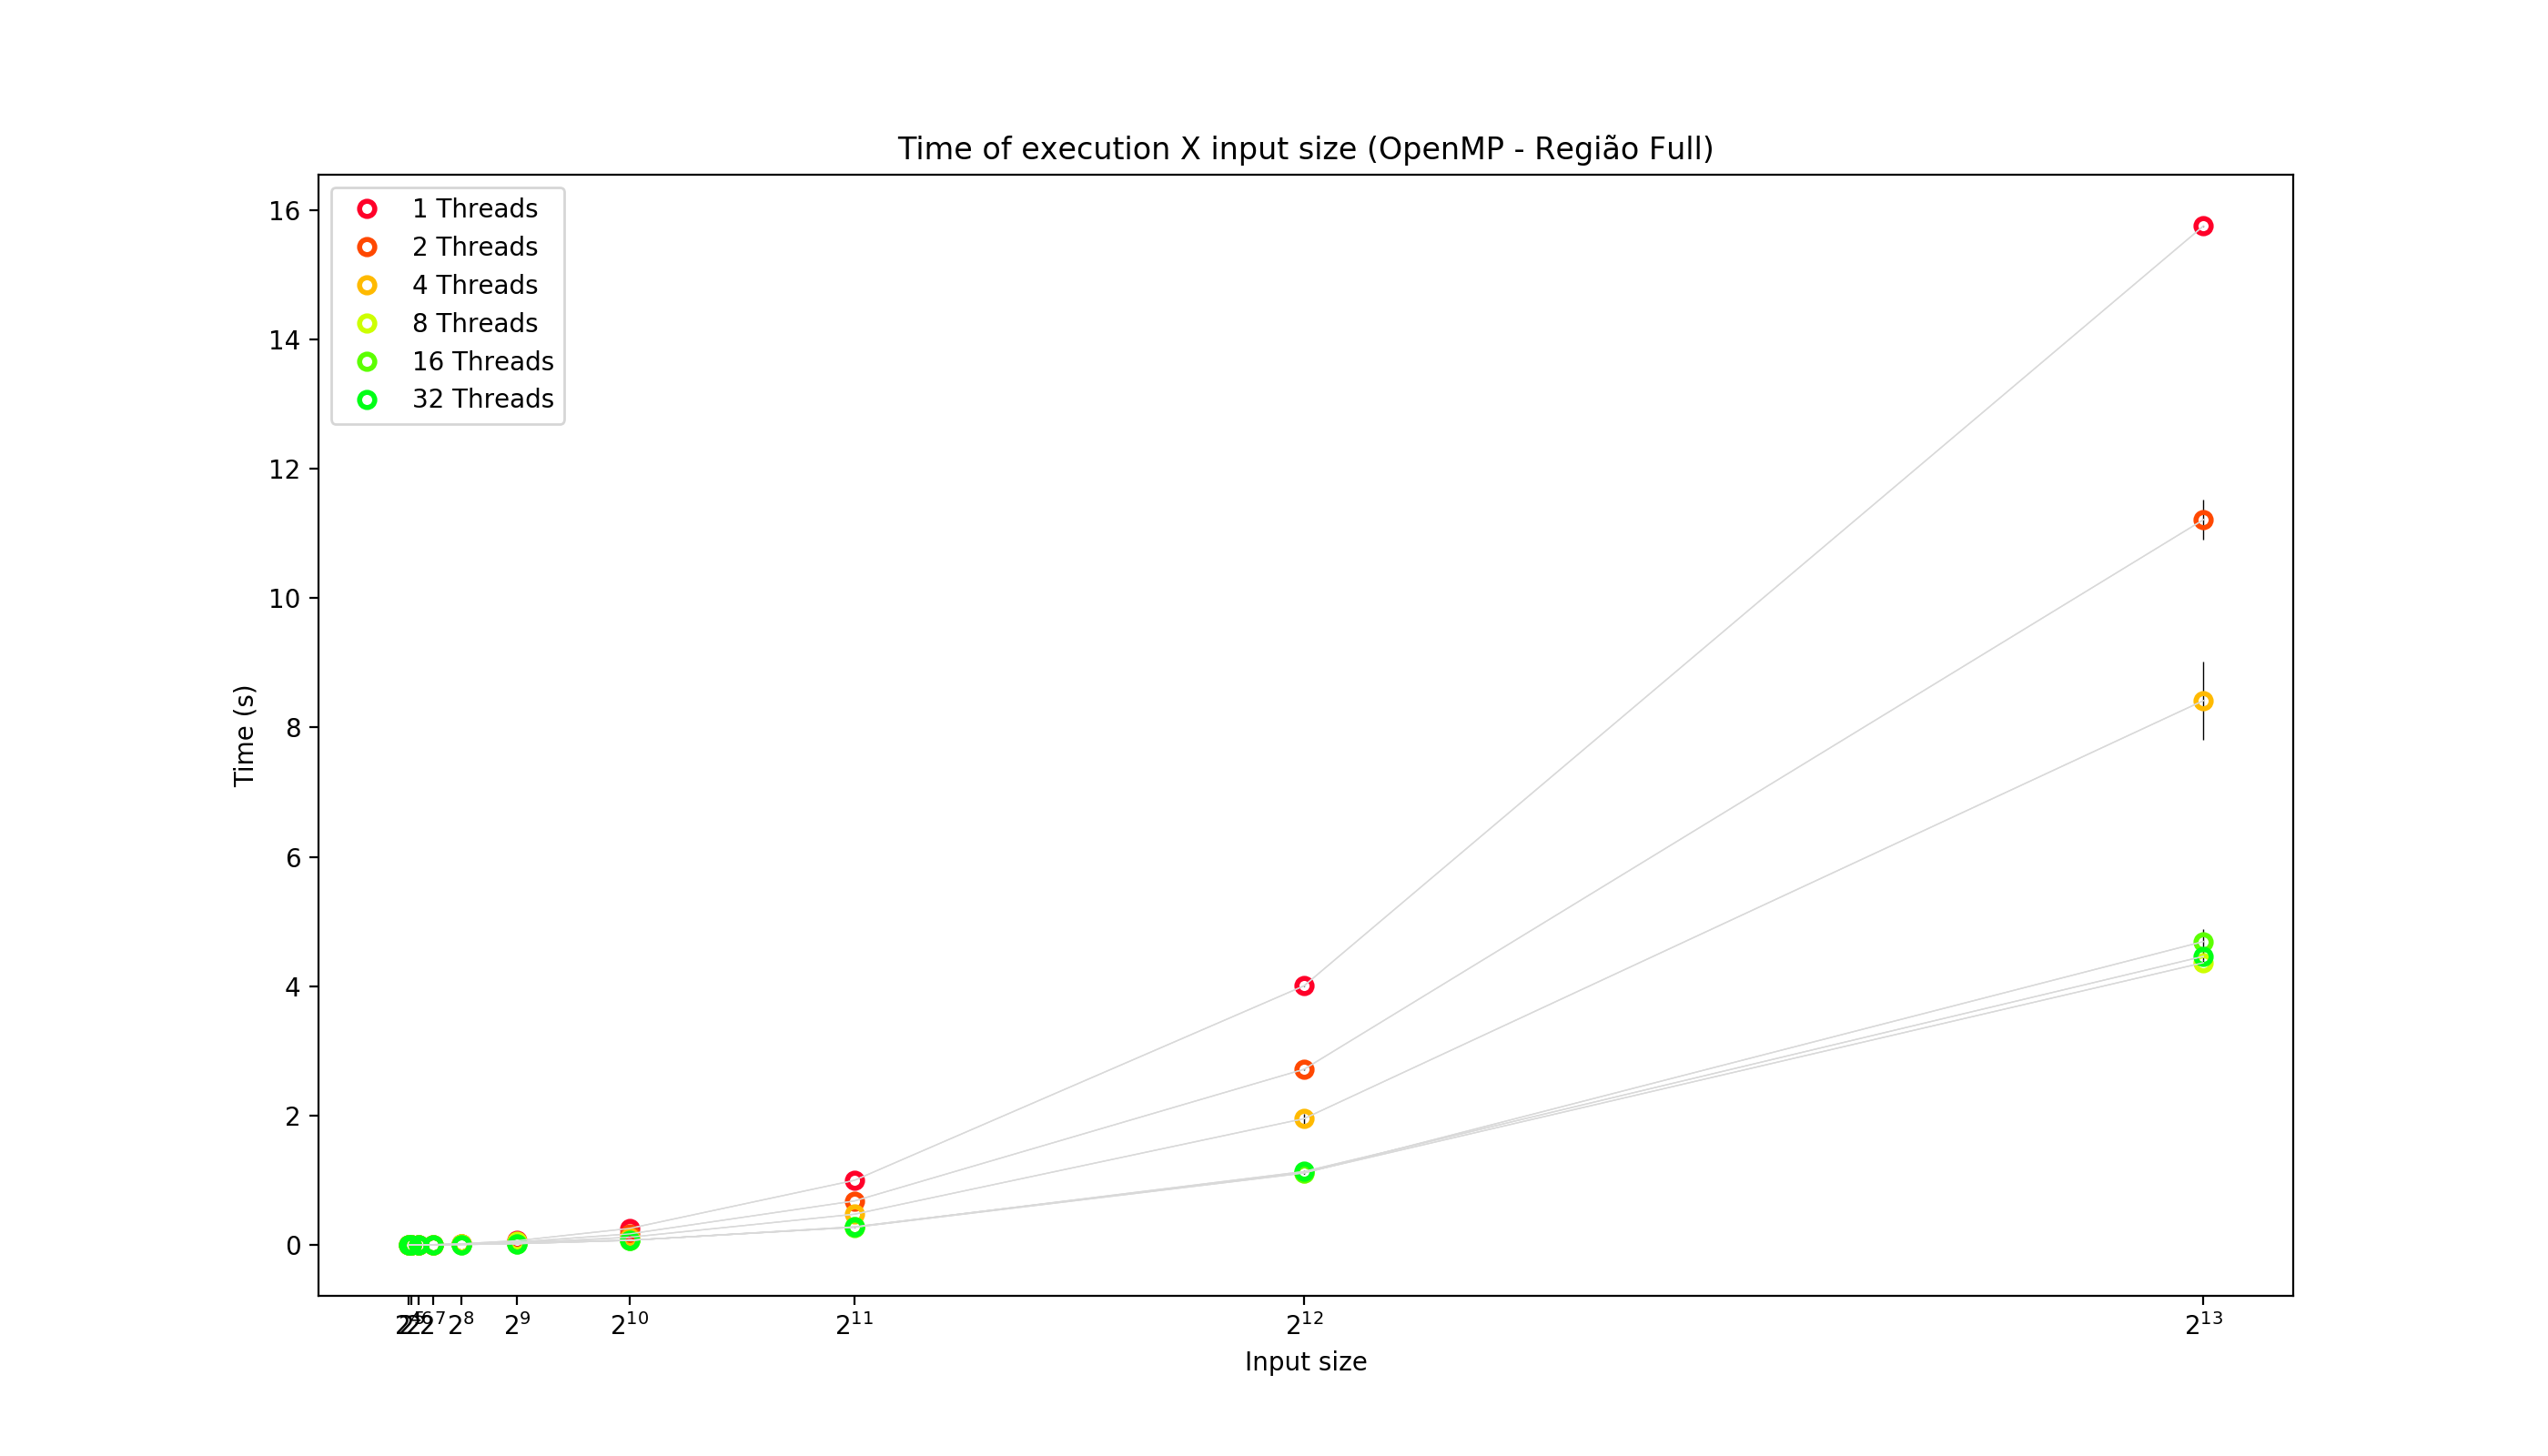
\includegraphics{omp_full/time_input_omp.png}}
            \label {fig:omp_full:B}
        }
        \\
        \subfigure[] {\scalebox{.20}{
            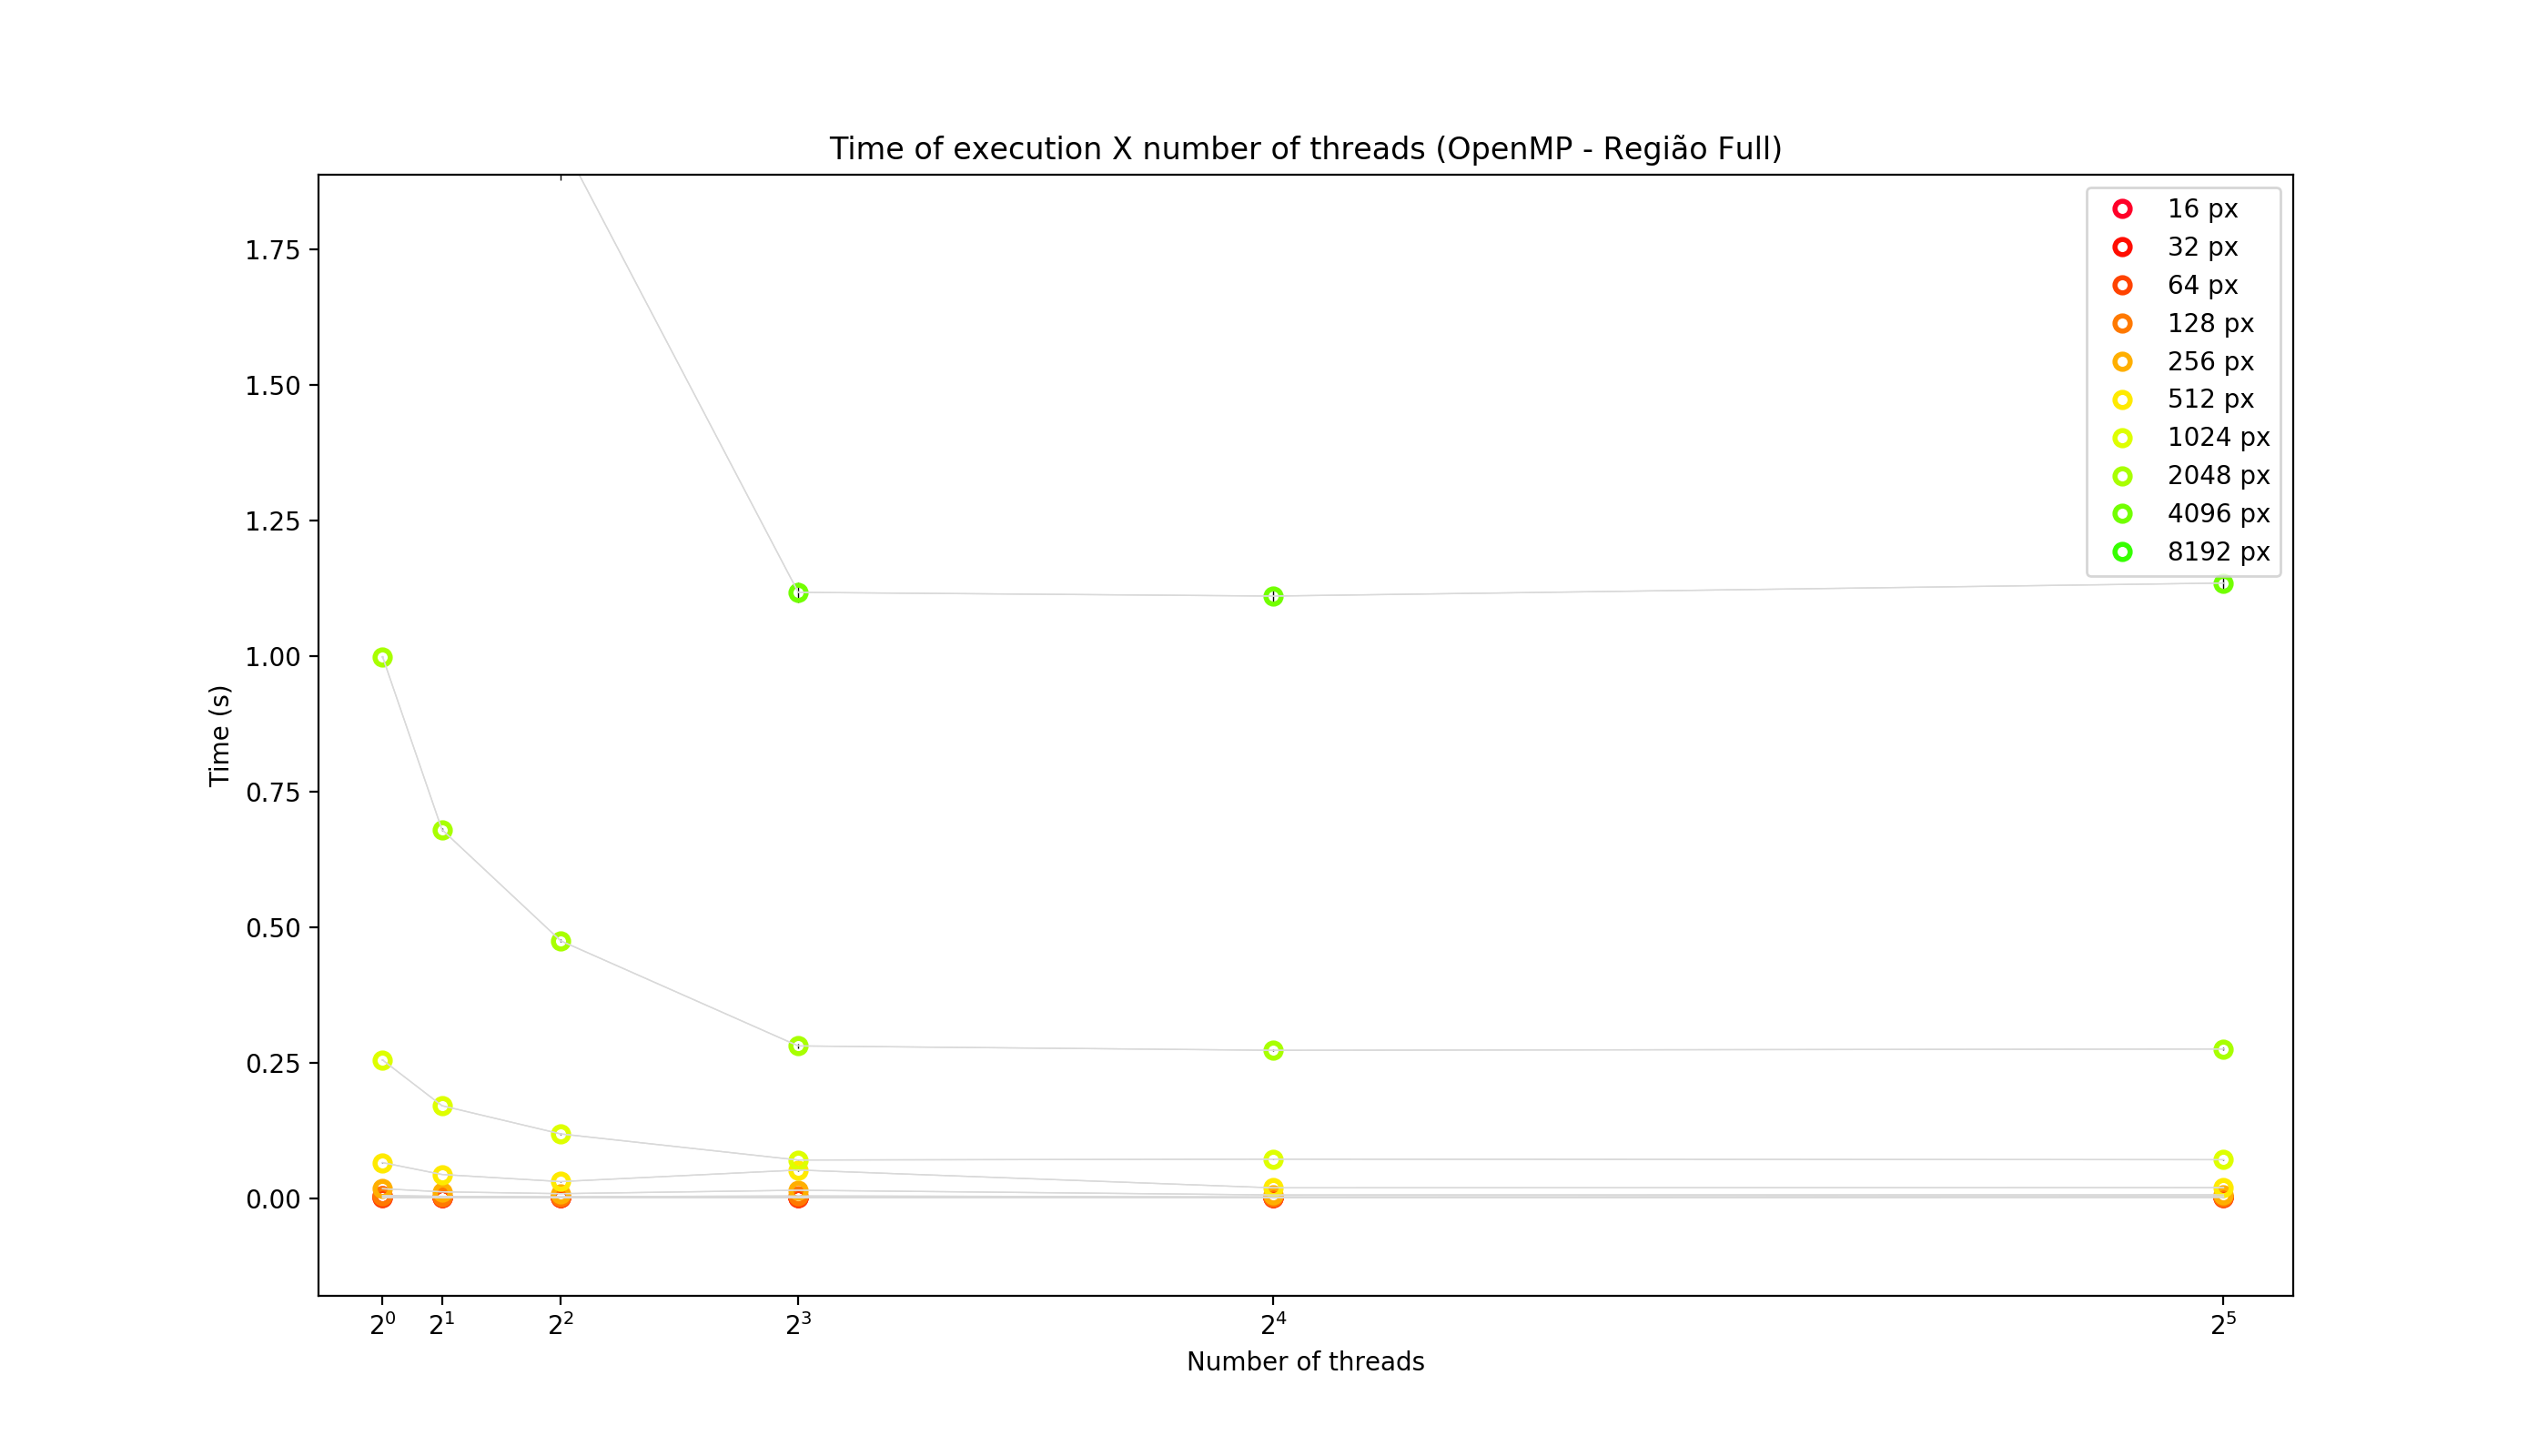
\includegraphics{omp_full/time_thread_omp_minor_values.png}}
            \label {fig:omp_full:C}
        }
        &
        \subfigure[] {\scalebox{.20}{
            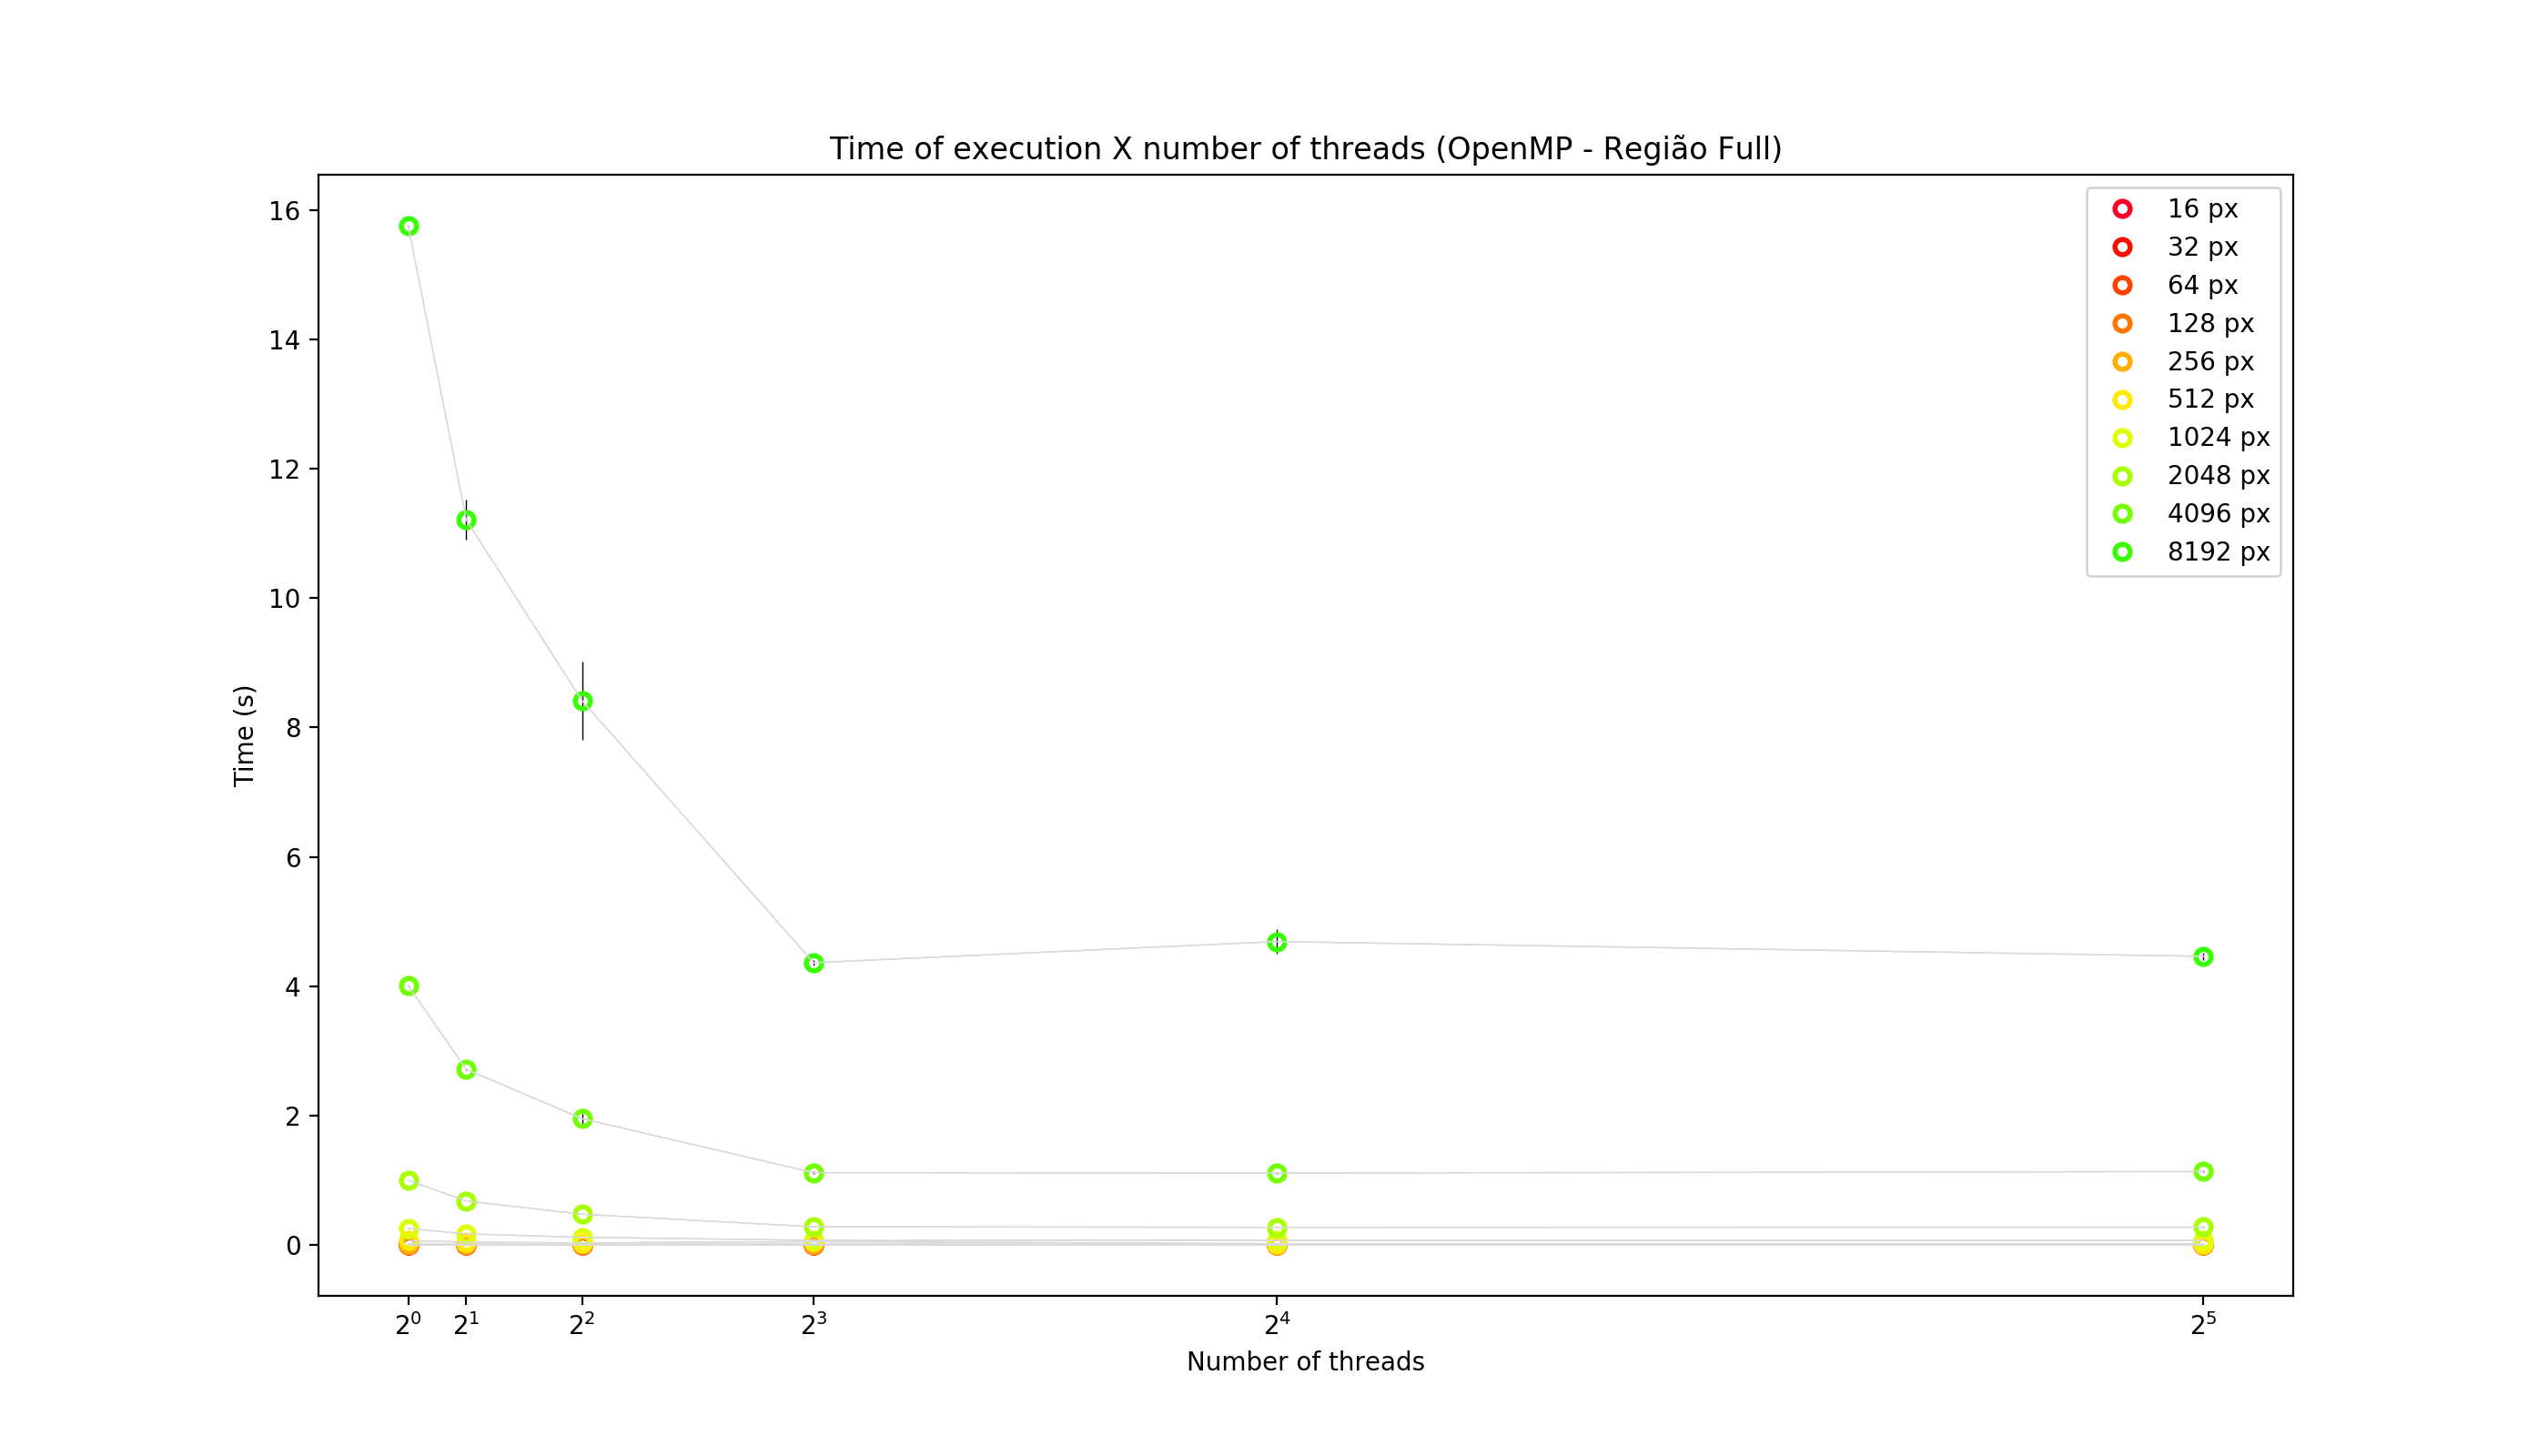
\includegraphics{omp_full/time_thread_omp.png}}
            \label {fig:omp_full:D}
        }
        
    \end{tabular}
    \caption{Temos a comparação de execução entre as 4 regiões do 
    conjunto.}
    \label{fig:omp_full} 
\end{figure}

\newpage


\newpage
\section{Conclusão}
\newpage

\end{document}
